\documentclass[10pt,prb,showpacs,amssymb,floatfix]{revtex4-1}
%\documentclass[10pt,prb,showpacs,floatfix,superscriptaddress]{revtex4-1}
%\usepackage{amsmath,amsbsy,graphics,epsfig,mathrsfs}
\usepackage{amsmath,amsbsy,graphics,epsfig}
\usepackage{bm}
\usepackage[]{color}

%%%%%% Definition of new commands for abbrevation%%%%%
% Fonts
\newcommand{\mbb}{\mathbb}
\newcommand{\mb}{\mathbb}
\newcommand{\mbf}{\mathbf}
\newcommand{\mac}{\mathcal}
\newcommand{\msc}{\mathscr}
\newcommand{\tx}{\text}
\newcommand{\ti}{\textit}
\newcommand{\tb}{\textbf}
\newcommand{\tsf}{\textsf}
\newcommand{\tm}{{\times}}
\newcommand{\noi}{\noindent}
% Symbols
\newcommand{\dg}{\dagger}
\newcommand{\daw}{\downarrow}
\newcommand{\dna}{\downarrow}
\newcommand{\dn}{\downarrow}
\newcommand{\Dna}{\Downarrow}
\newcommand{\la}{\langle}
\newcommand{\law}{\leftarrow}
\newcommand{\lra}{\leftrightarrow}
\newcommand{\nn}{\nonumber}
\newcommand{\pat}{\partial}
\newcommand{\para}{\parallel}
\newcommand{\pr}{\prime}
\newcommand{\ra}{\rangle}
\newcommand{\raw}{\rightarrow}
\newcommand{\til}{\tilde}
\newcommand{\upa}{\uparrow}
\newcommand{\up}{\uparrow}
\newcommand{\Upa}{\Uparrow}
\newcommand{\ub}{\underbrace}
\newcommand{\fr}{\frac}
%Greek letters
\newcommand{\alp}{\alpha}
\newcommand{\cp}{q}
\newcommand{\dlt}{\delta}
\newcommand{\Dlt}{\Delta}
\newcommand{\Dt}{\Delta}
\newcommand{\eps}{\epsilon}
\newcommand{\gm}{\gamma}
\newcommand{\Gm}{\Gamma}
\newcommand{\lam}{\lambda}
\newcommand{\Lam}{\Lambda}
\newcommand{\vp}{\varphi}
\newcommand{\tha}{\theta}
\newcommand{\vth}{\vartheta}
\newcommand{\vps}{\varepsilon}
\newcommand{\vs}{\varsigma}
\newcommand{\og}{\omega}
\newcommand{\Og}{\Omega}
\newcommand{\sg}{\sigma}
\newcommand{\Sg}{\Sigma}
\newcommand{\sig}{\sigma}
\newcommand{\kp}{\kappa}
\newcommand{\h}{\hat}
%Others
\newcommand{\etal}{{\em et al.,~}}
\newcommand{\ie}{{i.e.,~}}
%\usepackage{wrapfig}

\begin{document}
\title{Anomalous Hall effect in tunnel junctions}
\author{Collins Ashu Akosa}
\affiliation{Department of Applied Physics, Waseda University, Okubo, Shinjuku-ku, Tokyo 169-8555, Japan}
\affiliation{RIKEN Center for Emergent Matter Science (CEMS), 2-1 Hirosawa, Wako, Saitama 351-0198, Japan}
\affiliation{Department of Theoretical and Applied Physics, African University of Science and Technology (AUST), Km 10 Airport Road, Galadimawa, Abuja F.C.T, Nigeria}
%                                                                                                                                                                     
\author{Christian Ortiz Pauyac}
\affiliation{RIKEN Center for Emergent Matter Science (CEMS), 2-1 Hirosawa, Wako, Saitama 351-0198, Japan}
%                                                                                                                                                                     
%                                                                                                                                                                     
%\author{Sergey Nikolaev}                                                                                                                                             
%\affiliation{WRHI, Tokyo Institute of Technology, Yokohama 226-8503, Japan}                                                                                          
%                                                                                                                                                                     
\author{Mairbek Chshiev}
\affiliation{Univ. Grenoble Alpes, CNRS, CEA, Grenoble INP, INAC-SPINTEC, Grenoble 38000, France}

%\author{Alan Kalitsov}                                                                                                                                               
%\affiliation{Western Digital, San Jose, California 95131, USA}                                                                                                       
%                                                                                                                                                                     
\author{Gen Tatara}
\affiliation{RIKEN Center for Emergent Matter Science (CEMS), 2-1 Hirosawa, Wako, Saitama 351-0198, Japan}

\author{Masahito Mochizuki}
\affiliation{Department of Applied Physics, Waseda University, Okubo, Shinjuku-ku, Tokyo 169-8555, Japan}

\date{\today}

\begin{abstract}
We develop a simple model Hamiltonian for tunnel junctions in the presence of Rashba spin-orbit coupling. This model permits the direct calculation of anomalous Hall effect as well as other important effects such as ATMR, TAMR, Rashba torque, and SHE.
\end{abstract}
\pacs{10.1103.Jk}
\maketitle


\section{matrix elements}
In second quantization, a one dimensional operator $\hat O$ reads,

\begin{align}
\label{eq1}
\hat{O} &= \sum_{j,j',\sigma,\sigma'} T_{j,j'}^{\sigma,\sigma'} \hat{c}_{j'}^{\dagger \sigma'} \hat{c}^\sigma_j =  \sum_{j,j'} T_{j,j'}^{\uparrow,\uparrow} c_{j'}^{\dagger \uparrow} c_j^\uparrow + T_{j,j'}^{\uparrow,\downarrow} c_{j'}^{\dagger \downarrow} c_j^\uparrow + T_{j,j'}^{\downarrow,\uparrow} c_{j'}^{\dagger \uparrow} c_j^\downarrow + T_{j,j'}^{\downarrow,\downarrow} c_{j'}^{\dagger \downarrow} c_j^\downarrow.
\end{align}
       
           
              
$\hat{c}_{j'}^{\dagger \sigma'} (\hat{c}^\sigma_j)$ is the creation (annihilation) operator on site $j'$ ($j$) with spin index  $\sigma'(\sigma)$ and $T_{j,j'}^{\sigma,\sigma'}$ is the matrix element. To visualize the system, let's consider a chain of atoms, where each site is enumerated, see Fig. \ref{1d}. 

%%%%%%%%%
\begin{figure}[ht]
\centering
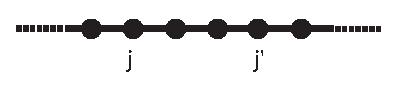
\includegraphics{fig1.eps}
\caption{One dimensional chain}
\label{1d}
\end{figure}
%%%%%%%%%%%   

The creation and annihilation operators in this system show the following properties,
\begin{align}
\label{pro1}
\hat{c}^\sigma_j \mid 0...1 0 0 0...0 , \sigma \rangle &=  \mid 0...0 0 0 0...0 \rangle, \\
\label{pro2}
\hat{c}^\sigma_j \mid 0...0 0 0 1...0 , \sigma \rangle &=  0,\\
\label{pro3}
\hat{c}_{j'}^{\dagger \sigma'} \mid 0...0 0 0 0...0\rangle &=  \mid 0...0 0 0 1...0, \sigma' \rangle.\\
\label{pro4}
\hat{c}_{j'}^{\dagger \sigma'} \mid 0...0 0 0 1...0\rangle &=  0, \\
\hat{c}_{j'}^{\dagger \sigma'} \mid 0...1 0 0 0...0\rangle &=  0.
\label{pro5}
\end{align}


$\mid 0...1 0 0 0...0 , \sigma \rangle$ represents the state where an electron with spin $\sigma$ exists at site $j$; therefore, it takes the value of 1 at this site and 0 in all the others. The operator $\hat{c}^\sigma_j$ destroys an electron on site $j$ with spin $\sigma$; therefore if we apply this operator to our state $\mid 0...1 0 0 0...0 , \sigma \rangle$, our new state becomes $ \mid 0...0 0 0 0...0 \rangle$, which is called the vacuum state, see Eq. \eqref{pro1}. If we instead apply the same operator to a system where the electron is on site $j'$ rather than $j$, then the result is zero as there is no electron to destroy on site $j$, see Eq. \eqref{pro2}. Similarly, if we consider the vacuum state, $ \mid 0...0 0 0 0...0 \rangle$, and apply the creation operator $\hat{c}_{j'}^{\dagger \sigma'}$, then we will create an electron on site $j'$ with spin $\sigma'$ and therefore our new state becomes $\mid 0...0 0 0 1...0, \sigma' \rangle$, see Eq. \eqref{pro3}. If an electron already exists on site $j'$ and we apply the creation operator then the result is zero as, in the present model, we cannot have two electrons on the same site, see Eq. \eqref{pro4}. In addition, if we apply the creation operator on site $j'$ considering a state that has already an electron on site $j$, the result is also zero as in the present model only one electron exists in the whole system, see Eq. \eqref{pro5}.  To simplify the notation we consider the following,
\begin{align}
\mid 0...1 0 0 0...0 , \sigma \rangle &= \mid j , \sigma \rangle, \\
\mid 0...0 0 0 1...0 , \sigma' \rangle  &=  \mid j' , \sigma' \rangle, \\
\mid 0...0 0 0 0...0 \rangle  &=  \mid 0 \rangle.
\end{align}


Considering Eq. \eqref{eq1} and the properties of the creation and annihilation operators we have, 

\begin{align}
\langle j',\sigma' \mid \hat{O} \mid j, \sigma \rangle &= \langle j',\sigma' \mid \sum_{n,m,\alpha,\alpha'} T_{n,m}^{\alpha,\alpha'} \hat{c}_m^{\dagger \alpha'} \hat{c}^\alpha_n \mid j, \sigma \rangle, \\
&= \langle j',\sigma' \mid \sum_{m,\alpha'} T_{j,m}^{\sigma,\alpha'} \hat{c}_m^{\dagger \alpha'} \hat{c}^\sigma_j \mid j, \sigma \rangle \\
&= \langle j',\sigma' \mid \sum_{m,\alpha'} T_{j,m}^{\sigma,\alpha'} \hat{c}_m^{\dagger \alpha'} \mid 0 \rangle, \\
&= \langle j',\sigma' \mid \sum_{m,\alpha'} T_{j,m}^{\sigma,\alpha'}  \mid m, \alpha' \rangle, \\
&= \sum_{m,\alpha'} T_{j,m}^{\sigma,\alpha'} \langle j',\sigma' \mid m, \alpha' \rangle, \\
&= T_{j,j'}^{\sigma,\sigma'} \langle j',\sigma' \mid j', \sigma' \rangle, \\
\langle j',\sigma' \mid \hat{O} \mid j, \sigma \rangle &= T_{j,j'}^{\sigma,\sigma'}.
\label{matel2} 
\end{align}

Consequently, in detail, the matrix elements are

\begin{align}
\label{matel30} 
T_{j,j'}^{\uparrow,\uparrow} = \langle j',\uparrow \mid \hat{O} \mid j, \uparrow \rangle, \\
\label{matel31} 
T_{j,j'}^{\uparrow,\downarrow} = \langle j',\downarrow \mid \hat{O} \mid j, \uparrow \rangle, \\
\label{matel32}
T_{j,j'}^{\downarrow,\uparrow} = \langle j',\uparrow \mid \hat{O} \mid j, \downarrow \rangle, \\
T_{j,j'}^{\downarrow,\downarrow} = \langle j',\downarrow \mid \hat{O} \mid j, \downarrow \rangle. 
\label{matel3} 
\end{align}

These results are the basis to derive any operator and its matrix elements in second quantization.

%%%%%%%%%%%%%%
\section{Hamiltonian Operator}
In the present work we study a magnetic tunnel junction in the presence of Rashba spin-orbit coupling. Transport is defined along the $y-$axis. The most general Hamiltonian for this system is given by,

\begin{align}
\h H = \h H_U + \h H_p + \h H_{\Dlt} + \h H_{so}.
\end{align}

$\h H_U$ appears in the barrier region only and is referred to as the potential Hamiltonian. $\h H_p$, present everywhere, is the kinetic Hamiltonian. The third term, $\h H_{\Dlt}$, present in magnetic layers only, is the exchange Hamiltonian, and the last term, $\h H_{so}$, is the spin-orbit coupling Hamiltonian, which appears at the interface of two samples for the particular case of Rashba spin-orbit coupling.

%%%%%%%%%%%%%%
\subsection{Potential Operator}

We first study the potential Hamiltonian. In first quantization we have,
\begin{align}
\hat H_{U} = U(y)
\label{U1st}
\end{align}

The matrix element notation, given in Eq.  \eqref{matel2} for a one dimensional case, can be extended to a three dimensional case. For the potential in the barrier region we have, 

\begin{align}
T_{ijk,i'j'k'}^{\sigma,\sigma'} = \langle i'j'k',\sigma' \mid \hat{H}_{U} \mid ijk, \sigma \rangle,
\end{align}

where subindexes ($i,i'$) run along the $x-$axis, ($j,j'$) along the $y-$axis, and ($k,k'$) along the $z-$axis. In its matrix form we have,

\begin{align}
&=  \big{(} \langle i'j'k',\uparrow \mid , \langle i'j'k',\downarrow \mid \big{)} \left(\begin{array}{cc} 
U(y) &  0\\
0 & U(y)
\end{array}\right)  \left(\begin{array}{c} 
\mid ijk,\uparrow \rangle \\
\mid ijk,\downarrow \rangle
\end{array}\right) \\
&= \langle i'j'k',\uparrow \mid U(y) \mid ijk,\uparrow \rangle +  \langle i'j'k',\downarrow \mid U(y) \mid ijk,\downarrow \rangle.
\label{eqU12}
\end{align}

Consequently, in analogy to Eqs. \eqref{matel30}-\eqref{matel3}, we have
 
\begin{align}
\label{eqU1220}
T_{ijk,i'j'k'}^{\uparrow,\uparrow} &= \langle i'j'k',\uparrow \mid U(y) \mid ijk,\uparrow \rangle, \\
\label{eqU1221}
T_{ijk,i'j'k'}^{\uparrow,\downarrow} &= 0, \\
\label{eqU1222}
T_{ijk,i'j'k'}^{\downarrow,\uparrow} &= 0, \\
T_{ijk,i'j'k'}^{\downarrow,\downarrow} &= \langle i'j'k',\downarrow \mid U(y) \mid ijk,\downarrow \rangle. 
\label{eqU123}
\end{align}

Applying Eq. \eqref{eq1} in our potential operator we get,

\begin{align}
\hat H_{U} &= \sum_{ijk,i'j'k',\sigma,\sigma'} T_{ijk,i'j'k'}^{\sigma,\sigma'} \hat{c}_{i'j'k'}^{\dagger \sigma'} \hat{c}_{ijk}^\sigma \\
&= \sum_{ijk,i'j'k'} T_{ijk,i'j'k'}^{\uparrow,\uparrow} c_{i'j'k'}^{\dagger \uparrow} c_{ijk}^\uparrow +  T_{ijk,i'j'k'}^{\uparrow,\downarrow} c_{i'j'k'}^{\dagger \downarrow} c_{ijk}^\uparrow + T_{ijk,i'j'k'}^{\downarrow,\uparrow} c_{i'j'k'}^{\dagger \uparrow} c_{ijk}^\downarrow + T_{ijk,i'j'k'}^{\downarrow,\downarrow} c_{i'j'k'}^{\dagger \downarrow} c_{ijk}^\downarrow.
\label{lastU}
\end{align}


Replacing Eqs. \eqref{eqU1220}-\eqref{eqU123} in Eq. \eqref{lastU} and summing over prime indices we have,

\begin{align}
\hat H_{U} &= \sum_{ijk,i'j'k'} \langle i'j'k',\uparrow \mid U(y) \mid ijk,\uparrow \rangle c_{i'j'k'}^{\dagger \uparrow} c_{ijk}^\uparrow  + \langle i'j'k',\downarrow \mid U(y) \mid ijk,\downarrow \rangle c_{i'j'k'}^{\dagger \downarrow} c_{ijk}^\downarrow \nn\\&= U(y) \sum_{ijk}  c_{ijk}^{\dagger \uparrow} c_{ijk}^\uparrow  +   c_{ijk}^{\dagger \downarrow} c_{ijk}^\downarrow
\label{lastU2}
\end{align}

Eq. \eqref{lastU2} refers to the potential operator in second quantization.

%%%%%%%%%%%%%%%%
\subsection{Exchange Operator}

In first quantization the s-d exchange interaction reads,
\begin{align}
\hat H_{\Dlt} = \Dlt \bm{\h \sigma}\cdot \bm m,
\label{sd1st}
\end{align}
$\Dlt$ is the exchange parameter, $\bm{\h \sigma} = (\sg_x, \sg_y, \sg_z)$ is the Pauli matrix vector, and $\bm m$ is the magnetization unit vector. We consider a random orientation of the magnetization vector; therefore, in spherical coordinates we have $\bm m = (\cos \phi \sin \theta, \sin\phi \sin\theta, \cos \theta)$. Considering,

\begin{align}
 {\sigma_x} = \begin{pmatrix} 0 & 1 \\ 1 & 0 \end{pmatrix} , ~  ~  ~  ~ {\sigma_y} = \begin{pmatrix} 0 & -i \\ i & 0 \end{pmatrix}, ~  ~  ~  ~   {\sigma_z} =  \begin{pmatrix} 1 & 0 \\ 0 & -1 \end{pmatrix}, 
\label{Pauli}
\end{align}

and the property, $e^{\pm i\phi} = \cos\phi \pm i \sin\phi$, we have,

\begin{equation}
\hat H_{\Dlt} =  \Dlt \left(\begin{array}{cc} 
\cos\theta & \sin\theta e^{-i\phi}\\
\sin\theta e^{i\phi} & -\cos\theta
\end{array}\right).
\label{sd1st2}
\end{equation}

The matrix element notation, given in Eq.  \eqref{matel2} for a one dimensional case can be extended to a three dimensional case. For the s-d exchange interaction we have, 

\begin{align}
T_{ijk,i'j'k'}^{\sigma,\sigma'} = \langle i'j'k',\sigma' \mid \hat{H}_{\Dlt} \mid ijk, \sigma \rangle
\end{align}

which in a matrix form can be given as,

\begin{align}
&=  \big{(} \langle i'j'k',\uparrow \mid , \langle i'j'k',\downarrow \mid \big{)} \left(\begin{array}{cc} 
\cos\theta &  \sin\theta e^{-i\phi}\\
 \sin\theta e^{i\phi} & -\cos\theta
\end{array}\right)  \left(\begin{array}{c} 
\mid ijk,\uparrow \rangle \\
\mid ijk,\downarrow \rangle
\end{array}\right) \\
&= \big{(}\langle i'j'k',\uparrow \mid , \langle i'j'k',\downarrow \mid \big{)}  \left(\begin{array}{c} 
\cos\theta  \mid ijk,\uparrow \rangle + \sin\theta e^{-i\phi}  \mid ijk,\downarrow \rangle \\
\sin\theta e^{i\phi} \mid ijk,\uparrow \rangle - \cos\theta \mid ijk,\downarrow \rangle
\end{array}\right) \\
&= \langle i'j'k',\uparrow \mid \cos\theta \mid ijk,\uparrow \rangle + \langle i'j'k',\uparrow \mid \sin\theta e^{-i\phi} \mid ijk,\downarrow \rangle +
 \langle i'j'k',\downarrow \mid \sin\theta e^{i\phi}\mid ijk,\uparrow \rangle -  \langle i'j'k',\downarrow \mid \cos\theta\mid ijk,\downarrow \rangle.
\label{eqsd12}
\end{align}

Consequently, in analogy to Eqs. \eqref{matel30}-\eqref{matel3}, we have
 
\begin{align}
\label{eqsd1220}
T_{ijk,i'j'k'}^{\uparrow,\uparrow} &= +\langle i'j'k',\uparrow \mid \cos\theta \mid ijk,\uparrow \rangle , \\
\label{eqsd1221}
T_{ijk,i'j'k'}^{\uparrow,\downarrow} &= +\langle i'j'k',\downarrow \mid \sin\theta e^{i\phi}  \mid ijk,\uparrow \rangle \\
\label{eqsd1222}
T_{ijk,i'j'k'}^{\downarrow,\uparrow} &= +\langle i'j'k',\uparrow \mid \sin\theta e^{-i\phi} \mid ijk,\downarrow \rangle, \\
T_{ijk,i'j'k'}^{\downarrow,\downarrow} &= -\langle i'j'k',\downarrow \mid \cos\theta \mid ijk,\downarrow \rangle. 
\label{eqsd123}
\end{align}

Applying Eq. \eqref{eq1} in our s-d exchange coupling operator, we get,

\begin{align}
\hat H_{\Dlt} &= \sum_{ijk,i'j'k',\sigma,\sigma'} T_{ijk,i'j'k'}^{\sigma,\sigma'} \hat{c}_{i'j'k'}^{\dagger \sigma'} \hat{c}_{ijk}^\sigma \\
&= \sum_{ijk,i'j'k'} T_{ijk,i'j'k'}^{\uparrow,\uparrow} c_{i'j'k'}^{\dagger \uparrow} c_{ijk}^\uparrow +  T_{ijk,i'j'k'}^{\uparrow,\downarrow} c_{i'j'k'}^{\dagger \downarrow} c_{ijk}^\uparrow + T_{ijk,i'j'k'}^{\downarrow,\uparrow} c_{i'j'k'}^{\dagger \uparrow} c_{ijk}^\downarrow + T_{ijk,i'j'k'}^{\downarrow,\downarrow} c_{i'j'k'}^{\dagger \downarrow} c_{ijk}^\downarrow.
\label{lastsd}
\end{align}

Replacing Eqs. \eqref{eqsd1220}-\eqref{eqsd123} in Eq. \eqref{lastsd} and summing over prime indices we have,

\begin{align}
\hat H_{\Dlt} &= \sum_{ijk,i'j'k'} \langle i'j'k',\uparrow \mid \cos\theta \mid ijk,\uparrow \rangle c_{i'j'k'}^{\dagger \uparrow} c_{ijk}^\uparrow +  \langle i'j'k',\downarrow \mid \sin\theta e^{i\phi}  \mid ijk,\uparrow \rangle c_{i'j'k'}^{\dagger \downarrow} c_{ijk}^\uparrow \nn\\ &~~~~~~~~~~+ \langle i'j'k',\uparrow \mid \sin\theta e^{-i\phi} \mid ijk,\downarrow \rangle c_{i'j'k'}^{\dagger \uparrow} c_{ijk}^\downarrow -\langle i'j'k',\downarrow \mid \cos\theta \mid ijk,\downarrow \rangle c_{i'j'k'}^{\dagger \downarrow} c_{ijk}^\downarrow \nn\\&= \sum_{ijk}  \cos\theta c_{ijk}^{\dagger \uparrow} c_{ijk}^\uparrow +  \sin\theta e^{i\phi} c_{ijk}^{\dagger \downarrow} c_{ijk}^\uparrow+  \sin\theta e^{-i\phi} c_{ijk}^{\dagger \uparrow} c_{ijk}^\downarrow - \cos\theta  c_{ijk}^{\dagger \downarrow} c_{ijk}^\downarrow
\label{lastsd2}
\end{align}

Eq. \eqref{lastsd2} refers to the s-d exchange interaction operator in second quantization.

%%%%%%%%%%%%%%
\subsection{Kinetic Operator}

In first quantization, the kinetic operator reads, 

\begin{align}
\hat H_{p} &= \frac{\bm p^2}{2m} \nn\\
&= -\frac{\hbar^2}{2m} (\partial_x^2 +\partial_y^2+\partial_z^2 ),
\label{p}
\end{align}

where $\bm p = -i\hbar\bm \nabla$. Before proceeding to retrieve the matrix elements of $\hat H_{p}$, we first discretize the differential operators, $\partial_i$ and $\partial_i^2$. To discretize $\partial_i$ we consider the following properties of derivatives based in Taylor expansion,

\begin{align}
\label{taylor1}
f(x_0 + h) = f(x_0) + h f'(x_0) + h^2 f''(x_0) / 2, \\
f(x_0 - h) = f(x_0) - h f'(x_0) + h^2 f''(x_0) / 2.
\label{taylor2}
\end{align}
Subtracting Eqs. \eqref{taylor1} and \eqref{taylor2},

\begin{align}
lim_{h\rightarrow 0}\frac{f(x_0 + h) - f(x_0 - h)}{2h} = f'(x_0) = \partial_x f(x) \big{|}_{x=x_0}.
\label{taylor3}
\end{align}

Therefore, for a discrete system we have,

\begin{align}
\frac{f_{i+1} - f_{i-1}}{2a} =  \partial_x f_i 
\label{taylor4}
\end{align}

where $a$ is the distance from one site to the next one. Eq. \eqref{taylor4} tells us that the first order differential operator applied on $i$ can be expressed as the difference of states in $i+1$ and $i-1$. The same analysis holds for the $y-$ and $z-$ components,

\begin{align}
\frac{f_{j+1} - f_{j-1}}{2a} =  \partial_y f_j, \\
\frac{f_{k+1} - f_{k-1}}{2a} =  \partial_z f_k. 
\label{taylor5}
\end{align}

The second order differential operator appears by summing up Eqs. \eqref{taylor1} and \eqref{taylor2},

\begin{align}
lim_{h\rightarrow 0}\frac{f(x_0 + h) +  f(x_0 - h) - 2f(x_0)}{h^2} = f''(x_0) = \partial^2_x f(x) \big{|}_{x=x_0}.
\label{taylor6}
\end{align}

Therefore for a discrete system we have,

\begin{align}
\frac{f_{i+1} + f_{i-1} - 2f_i}{a^2} =  \partial^2_x f_i 
\label{taylor7}
\end{align}

The same analysis holds for the $y-$ and $z-$ components,

\begin{align}
\frac{f_{j+1} + f_{j-1} - 2f_j}{a^2} =  \partial^2_y f_j, \\
\frac{f_{k+1} + f_{k-1} - 2f_k}{a^2} =  \partial^2_z f_k. 
\label{taylor8}
\end{align}

Having defined the differential operators, we now proceed to retrieve the matrix elements. We have, 

\begin{align}
T_{ijk,i'j'k'}^{\sigma,\sigma'} = \langle i'j'k',\sigma' \mid \hat{H}_{p} \mid ijk, \sigma \rangle,
\end{align}

which in its matrix form is given by,

\begin{align}
&=  \big{(} \langle i'j'k',\uparrow \mid , \langle i'j'k',\downarrow \mid \big{)} \left(\begin{array}{cc} 
-\frac{\hbar^2}{2m} (\partial_x^2 +\partial_y^2+\partial_z^2 ) &  0\\
0 & -\frac{\hbar^2}{2m} (\partial_x^2 +\partial_y^2+\partial_z^2 )
\end{array}\right)  \left(\begin{array}{c} 
\mid ijk,\uparrow \rangle \\
\mid ijk,\downarrow \rangle
\end{array}\right) \\
&= \langle i'j'k',\uparrow \mid -\frac{\hbar^2}{2m} (\partial_x^2 +\partial_y^2+\partial_z^2 ) \mid ijk,\uparrow \rangle +  \langle i'j'k',\downarrow \mid -\frac{\hbar^2}{2m} (\partial_x^2 +\partial_y^2+\partial_z^2 ) \mid ijk,\downarrow \rangle.
\label{eqP12}
\end{align}

Consequently, in analogy to Eqs. \eqref{matel30}-\eqref{matel3}, we have
 
\begin{align}
\label{eqP1220}
T_{ijk,i'j'k'}^{\uparrow,\uparrow} &= \langle i'j'k',\uparrow \mid -\frac{\hbar^2}{2m} (\partial_x^2 +\partial_y^2+\partial_z^2 ) \mid ijk,\uparrow \rangle, \\
\label{eqP1221}
T_{ijk,i'j'k'}^{\uparrow,\downarrow} &= 0, \\
\label{eqP1222}
T_{ijk,i'j'k'}^{\downarrow,\uparrow} &= 0, \\
T_{ijk,i'j'k'}^{\downarrow,\downarrow} &= \langle i'j'k',\downarrow \mid -\frac{\hbar^2}{2m} (\partial_x^2 +\partial_y^2+\partial_z^2 ) \mid ijk,\downarrow \rangle. 
\label{eqP123}
\end{align}

Replacing the second-order differential operators given in Eqs. \eqref{taylor7}-\eqref{taylor8} we get,

\begin{align}
\label{eqP12200}
T_{ijk,i'j'k'}^{\uparrow,\uparrow} &= \langle i'j'k',\uparrow \mid -\frac{\hbar^2}{2m} (\partial_x^2 +\partial_y^2+\partial_z^2 ) \mid ijk,\uparrow \rangle, \nn\\
&= -\frac{\hbar^2}{2m}[ \langle i'j'k',\uparrow \mid \partial_x^2 \mid ijk,\uparrow \rangle + \langle i'j'k',\uparrow \mid \partial_y^2 \mid ijk,\uparrow \rangle + \langle i'j'k',\uparrow \mid \partial_z^2 \mid ijk,\uparrow \rangle] \nn\\
&=-\frac{\hbar^2}{2ma^2}[ \langle i'j'k',\uparrow \mid i+1jk,\uparrow \rangle + \langle i'j'k',\uparrow \mid i-1jk,\uparrow \rangle - 2 \langle i'j'k',\uparrow \mid ijk,\uparrow \rangle \nn\\ &~~~~~~~~~~~+ \langle i'j'k',\uparrow \mid  ij+1k,\uparrow \rangle +  \langle i'j'k',\uparrow \mid  ij-1k,\uparrow \rangle - 2 \langle i'j'k',\uparrow \mid  ijk,\uparrow \rangle \nn\\&~~~~~~~~~~~+ \langle i'j'k',\uparrow  \mid ijk+1,\uparrow \rangle+  \langle i'j'k',\uparrow  \mid ijk-1,\uparrow \rangle - 2 \langle i'j'k',\uparrow  \mid ijk,\uparrow \rangle], \\
\label{eqP12211}
T_{ijk,i'j'k'}^{\uparrow,\downarrow} &= 0, \\
\label{eqP12222}
T_{ijk,i'j'k'}^{\downarrow,\uparrow} &= 0, \\
T_{ijk,i'j'k'}^{\downarrow,\downarrow} &= -\frac{\hbar^2}{2ma^2}[ \langle i'j'k',\downarrow \mid i+1jk,\downarrow \rangle + \langle i'j'k',\downarrow \mid i-1jk,\downarrow \rangle - 2 \langle i'j'k',\downarrow \mid ijk,\downarrow \rangle \nn\\ &~~~~~~~~~~~+ \langle i'j'k',\downarrow \mid  ij+1k,\downarrow \rangle +  \langle i'j'k',\downarrow \mid  ij-1k,\downarrow \rangle - 2 \langle i'j'k',\downarrow \mid  ijk,\downarrow \rangle \nn\\&~~~~~~~~~~~+ \langle i'j'k',\downarrow  \mid ijk+1,\downarrow \rangle+  \langle i'j'k',\downarrow  \mid ijk-1,\downarrow \rangle - 2 \langle i'j'k',\downarrow  \mid ijk,\downarrow \rangle]. 
\label{eqP1233}
\end{align}

Applying Eq. \eqref{eq1} in our kinetic operator, we get,

\begin{align}
\hat H_{p} &= \sum_{ijk,i'j'k',\sigma,\sigma'} T_{ijk,i'j'k'}^{\sigma,\sigma'} \hat{c}_{i'j'k'}^{\dagger \sigma'} \hat{c}_{ijk}^\sigma, \nn\\
&= \sum_{ijk,i'j'k'} T_{ijk,i'j'k'}^{\uparrow,\uparrow} c_{i'j'k'}^{\dagger \uparrow} c_{ijk}^\uparrow +  T_{ijk,i'j'k'}^{\uparrow,\downarrow} c_{i'j'k'}^{\dagger \downarrow} c_{ijk}^\uparrow + T_{ijk,i'j'k'}^{\downarrow,\uparrow} c_{i'j'k'}^{\dagger \uparrow} c_{ijk}^\downarrow + T_{ijk,i'j'k'}^{\downarrow,\downarrow} c_{i'j'k'}^{\dagger \downarrow} c_{ijk}^\downarrow, \nn\\
&= \sum_{ijk,i'j'k'} T_{ijk,i'j'k'}^{\uparrow,\uparrow} c_{i'j'k'}^{\dagger \uparrow} c_{ijk}^\uparrow  + T_{ijk,i'j'k'}^{\downarrow,\downarrow} c_{i'j'k'}^{\dagger \downarrow} c_{ijk}^\downarrow.
\label{lastxzP}
\end{align}

Replacing  Eqs. \eqref{eqP12200}-\eqref{eqP1233} in Eq. \eqref{lastxzP} and summing over $i'$, $j'$, and $k'$, then

\begin{align}
\hat H_{p} &= -\frac{\hbar^2}{2ma^2} \sum_{ijk}  \Big{[} c_{i+1jk}^{\dagger \uparrow} c_{ijk}^\uparrow + c_{i-1jk}^{\dagger \uparrow} c_{ijk}^\uparrow   + c_{ij+1k}^{\dagger \uparrow} c_{ijk}^\uparrow +c_{ij-1k}^{\dagger \uparrow} c_{ijk}^\uparrow   + c_{ijk+1}^{\dagger \uparrow} c_{ijk}^\uparrow + c_{ijk-1}^{\dagger \uparrow} c_{ijk}^\uparrow  -6 c_{ijk}^{\dagger \uparrow} c_{ijk}^\uparrow \nn\\
& ~~~~~~~~~~~~~~~~~+ c_{i+1jk}^{\dagger \downarrow} c_{ijk}^\downarrow + c_{i-1jk}^{\dagger \downarrow} c_{ijk}^\downarrow   + c_{ij+1k}^{\dagger \downarrow} c_{ijk}^\downarrow +c_{ij-1k}^{\dagger \downarrow} c_{ijk}^\downarrow   + c_{ijk+1}^{\dagger \downarrow} c_{ijk}^\downarrow + c_{ijk-1}^{\dagger \downarrow} c_{ijk}^\downarrow  -6 c_{ijk}^{\dagger \downarrow} c_{ijk}^\downarrow\Big{]} \\ 
&=  -\frac{\hbar^2}{2ma^2} \sum_{ijk,\sg}  \Big{[} c_{i+1jk}^{\dagger \sg} c_{ijk}^\sg + c_{i-1jk}^{\dagger \sg} c_{ijk}^\sg   + c_{ij+1k}^{\dagger \sg} c_{ijk}^\sg +c_{ij-1k}^{\dagger \sg} c_{ijk}^\sg   + c_{ijk+1}^{\dagger \sg} c_{ijk}^\sg + c_{ijk-1}^{\dagger \sg} c_{ijk}^\sg  -6 c_{ijk}^{\dagger \sg} c_{ijk}^\sg \Big{]} 
\end{align}
Considering that we are summing up over a huge number of atomic sites, subindexes can be modified as follow,
\begin{align}
\hat H_{p} &=  -\frac{\hbar^2}{2ma^2} \sum_{ijk,\sg}  \Big{[} c_{i+1jk}^{\dagger \sg} c_{ijk}^\sg + c_{ijk}^{\dagger \sg} c_{i+1jk}^\sg   + c_{ij+1k}^{\dagger \sg} c_{ijk}^\sg +c_{ijk}^{\dagger \sg} c_{ij+1k}^\sg   + c_{ijk+1}^{\dagger \sg} c_{ijk}^\sg + c_{ijk}^{\dagger \sg} c_{ijk+1}^\sg  -6 c_{ijk}^{\dagger \sg} c_{ijk}^\sg \Big{]} \nn\\
&=  -\frac{\hbar^2}{2ma^2} \sum_{ijk,\sg}  \Big{[} c_{i+1jk}^{\dagger \sg} c_{ijk}^\sg    + c_{ij+1k}^{\dagger \sg} c_{ijk}^\sg   + c_{ijk+1}^{\dagger \sg} c_{ijk}^\sg   -3 c_{ijk}^{\dagger \sg} c_{ijk}^\sg + h.c.  \Big{]},
\label{hpoperator}
\end{align}

where $h.c.$ is the Hermitian conjugate. Eq. \eqref{hpoperator} refers to the kinetic operator in second quantization.

%%%%%%%%%%%%%%%%
\subsection{Rashba spin-orbit coupling Operator along the xz-plane}
\label{sec:rashbaxz}

In first quantization, Rashba spin-orbit coupling in a 2DEG along the $xz-$plane reads 

\begin{align}
\hat H_{so} &= \lam_{so}(\bm y \times \bm k)\cdot \bm \sg \nn\\&
= \lambda_{so} (\sigma_x k_z - \sigma_z k_x) 
\label{alpxz}
\end{align}

where $\sigma_i$ denotes the Pauli matrix element given in Eq. \eqref{Pauli}, $p_i=\hbar k_i = -i\hbar \partial_i$ is the momentum, and $\lambda_{so}$ is the Rashba coefficient. Replacing these values we have,

\begin{equation}
\hat H_{so} =  i\lambda_{so} \left(\begin{array}{cc} 
\partial_x  &  -\partial_z\\
-\partial_z &  -\partial_x 
\end{array}\right).
\label{eq11xz}
\end{equation}

Taking $i\lam_{so} = \lam_{so}^*$, the matrix elements are,

\begin{align}
&=  \big{(} \langle i'k',\uparrow \mid , \langle i'k',\downarrow \mid \big{)} \left(\begin{array}{cc} 
\lambda_{so}^* \partial_x &  -\lambda_{so}^* \partial_z\\
 -\lambda_{so}^*\partial_z & -\lambda_{so}^* \partial_x
\end{array}\right)  \left(\begin{array}{c} 
\mid ik,\uparrow \rangle \\
\mid ik,\downarrow \rangle
\end{array}\right) \\
&= \big{(}\langle i'k',\uparrow \mid , \langle i'k',\downarrow \mid \big{)}  \left(\begin{array}{c} 
\lambda_{so}^*(\partial_x) \mid ik,\uparrow \rangle-\lambda_{so}^*(\partial_z) \mid ik,\downarrow \rangle \\
-\lambda_{so}^*(\partial_z) \mid ik,\uparrow \rangle - \lambda_{so}^*(\partial_x) \mid ik,\downarrow \rangle
\end{array}\right) \\
&= \langle i'k',\uparrow \mid  \lambda_{so}^*(\partial_x) \mid ik,\uparrow \rangle - \langle i'k',\uparrow \mid  \lambda_{so}^*(\partial_z) \mid ik,\downarrow \rangle -
 \langle i'k',\downarrow \mid \lambda_{so}^*(\partial_z) \mid ik,\uparrow \rangle - \langle i'k',\downarrow \mid \lambda_{so}^*(\partial_x) \mid ik,\downarrow \rangle,
\label{eq12xz}
\end{align}

where $i(k)$ and $i'(k')$ correspond to site enumeration along $x(z)-$axis. Notice that $j$-index is omitted as the system remains constant along the $y-$axis. 

In detail we have,

\begin{align}
\label{eq1220xz}
T_{ik,i'k'}^{\uparrow,\uparrow} &= +\langle i'k',\uparrow \mid  \lambda_{so}^*(\partial_x) \mid ik,\uparrow \rangle, \\
\label{eq1221xz}
T_{ik,i'k'}^{\uparrow,\downarrow} &= -\langle i'k',\downarrow \mid \lambda_{so}^*(\partial_z) \mid ik,\uparrow \rangle \\
\label{eq1222xz}
T_{ik,i'k'}^{\downarrow,\downarrow} &= - \langle i'k',\downarrow \mid \lambda_{so}^*(\partial_x) \mid ik,\downarrow \rangle, \\
T_{ik,i'k'}^{\downarrow,\uparrow} &= -\langle i'k',\uparrow \mid  \lambda_{so}^*(\partial_z) \mid ik,\downarrow \rangle.
\label{eq122xz}
\end{align}

Replacing the first-order differential operators given in Eqs. \eqref{taylor4}  and \eqref{taylor5} we get,

\begin{align}
\label{eq1220xz2}
T_{ik,i'k'}^{\uparrow,\uparrow} &= \frac{\lambda_{so}^*}{2a}  \big{(}\langle i'k',\uparrow \mid i+1k,\uparrow \rangle - \langle i'k',\uparrow \mid i-1k,\uparrow \rangle\big{)}, \\
\label{eq1221xz2}
T_{ik,i'k'}^{\uparrow,\downarrow} &= \frac{\lambda_{so}^*}{2a} \big{(} -\langle i'k',\downarrow \mid ik+1,\uparrow \rangle +\langle i'k',\downarrow \mid ik-1,\uparrow \rangle  \big{)}\\
\label{eq1222xz2}
T_{ik,i'k'}^{\downarrow,\downarrow} &= \frac{\lambda_{so}^*}{2a} \big{(} - \langle i'k',\downarrow  \mid i+1k,\downarrow \rangle + \langle i'k',\downarrow \mid i-1k,\downarrow \rangle \big{)}, \\
T_{ik,i'k'}^{\downarrow,\uparrow} &= \frac{\lambda_{so}^*}{2a} \big{(} -\langle i'k',\uparrow \mid ik+1,\downarrow \rangle +  \langle i'k',\uparrow \mid ik-1,\downarrow \rangle \big{)}.
\label{eq122xz2}
\end{align}

Applying Eq. \eqref{eq1} in our Rashba operator, we get,

\begin{align}
\hat H_{so} &= \sum_{ik,i'k',\sigma,\sigma'} T_{ik,i'k'}^{\sigma,\sigma'} \hat{c}_{i'k'}^{\dagger \sigma'} \hat{c}_{ik}^\sigma \nn\\
&= \sum_{ik,i'k'} T_{ik,i'k'}^{\uparrow,\uparrow} c_{i'k'}^{\dagger \uparrow} c_{ik}^\uparrow +  T_{ik,i'k'}^{\uparrow,\downarrow} c_{i'k'}^{\dagger \downarrow} c_{ik}^\uparrow + T_{ik,i'k'}^{\downarrow,\uparrow} c_{i'k'}^{\dagger \uparrow} c_{ik}^\downarrow + T_{ik,i'k'}^{\downarrow,\downarrow} c_{i'k'}^{\dagger \downarrow} c_{ik}^\downarrow.
\label{lastxz}
\end{align}

Replacing  Eqs. \eqref{eq1220xz2}-\eqref{eq122xz2} in Eq. \eqref{lastxz} and summing over $i'$ and $k'$, then

\begin{align}
\hat H_{so} &= \sum_{ik} \frac{\lambda_{so}^*}{2a} \Big{[} \big{(}c_{i+1k}^{\dagger \uparrow} c_{ik}^\uparrow - c_{i-1k}^{\dagger \uparrow} c_{ik}^\uparrow\big{)} +  \big{(} - c_{ik+1}^{\dagger \downarrow} c_{ik}^\uparrow + c_{ik-1}^{\dagger \downarrow} c_{ik}^\uparrow  \big{)} +  \big{(} - c_{ik+1}^{\dagger \uparrow} c_{ik}^\downarrow +  c_{ik-1}^{\dagger \uparrow} c_{ik}^\downarrow \big{)} +  \big{(} - c_{i+1k}^{\dagger \downarrow} c_{ik}^\downarrow + c_{i-1k}^{\dagger \downarrow} c_{ik}^\downarrow \big{)}  \Big{]} \nn\\
&= \sum_{ik} \frac{\lambda_{so}^*}{2a} \Big{[} \big{(}c_{i+1k}^{\dagger \uparrow} c_{ik}^\uparrow - c_{ik}^{\dagger \uparrow} c_{i+1k}^\uparrow\big{)} +  \big{(} -c_{ik+1}^{\dagger \downarrow} c_{ik}^\uparrow + c_{ik}^{\dagger \downarrow} c_{ik+1}^\uparrow  \big{)} +  \big{(} -c_{ik+1}^{\dagger \uparrow} c_{ik}^\downarrow +  c_{ik}^{\dagger \uparrow} c_{ik+1}^\downarrow \big{)} +  \big{(} - c_{i+1k}^{\dagger \downarrow} c_{ik}^\downarrow + c_{ik}^{\dagger \downarrow} c_{i+1k}^\downarrow \big{)}  \Big{]} \nn\\
&= \sum_{ik} \frac{\lambda_{so}}{2a} \Big{[} \big{(}i c_{i+1k}^{\dagger \uparrow}  c_{ik}^\uparrow - i c_{ik}^{\dagger \uparrow}  c_{i+1k}^\uparrow  - i c_{i+1k}^{\dagger \downarrow}  c_{ik}^\downarrow + i c_{ik}^{\dagger \downarrow}  c_{i+1k}^\downarrow \big{)} +  \big{(} - i c_{ik+1}^{\dagger \downarrow}  c_{ik}^\uparrow + i c_{ik}^{\dagger \downarrow}  c_{ik+1}^\uparrow   - i c_{ik+1}^{\dagger \uparrow}  c_{ik}^\downarrow +  i c_{ik}^{\dagger \uparrow}  c_{ik+1}^\downarrow \big{)}  \Big{]} \nn\\
&= \sum_{ik} \frac{\lambda_{so}}{2a} \Big{[} \big{(}i c_{i+1k}^{\dagger \uparrow} c_{ik}^\uparrow  - i c_{i+1k}^{\dagger \downarrow} c_{ik}^\downarrow + h.c. \big{)} +  \big{(} -i c_{ik+1}^{\dagger \downarrow}  c_{ik}^\uparrow  - i c_{ik+1}^{\dagger \uparrow}  c_{ik}^\downarrow + h.c. \big{)}  \Big{]}
\label{hsooperator}
\end{align}

Eq. \eqref{hsooperator} refers to the Rashba spin-orbit coupling operator along the $xz-$plane in second quantization.

%%%%%%%%%%%%%%%%%%%%
\subsubsection{Rashba Matrix Elements}
\label{sec:rashbamatrix}

In Eq. \eqref{hsooperator} the first (second) term considers creation and annihilation operations on sites along the $x(z)-$axis only; therefore, we can separate the solution in two parts,

\begin{align}
\label{hsoxx0}
\hat H^X_{so} &= \sum_{i} \frac{\lambda_{so}^*}{2a}  \Bigg{\{} c_{i+1}^{\dagger \uparrow} c_{i}^\uparrow - c_{i}^{\dagger \uparrow} c_{i+1}^\uparrow  - c_{i+1}^{\dagger \downarrow} c_{i}^\downarrow + c_{i}^{\dagger \downarrow} c_{i+1}^\downarrow \Bigg{\}}, \\
\hat H^Z_{so} &= \sum_{k}  \frac{\lambda_{so}^*}{2a} \Bigg{\{} - c_{k+1}^{\dagger \downarrow} c_{k}^\uparrow + c_{k}^{\dagger \downarrow} c_{k+1}^\uparrow   - c_{k+1}^{\dagger \uparrow} c_{k}^\downarrow +  c_{k}^{\dagger \uparrow} c_{k+1}^\downarrow \Bigg{\}}.
\label{hsozz0}
\end{align}

Notice in the above equations that we have supressed the second sub-index for simplicity as it remains unchanged; however, we should keep in mind this for future calculations.

The Bloch wave function in a two dimensional crystal is given by

\begin{align}
\mid \psi^\sigma_{\bf k} \rangle &= \frac{1}{\sqrt{N_x}}\frac{1}{\sqrt{N_z}} \sum_{l, n} e^{ik_xla}e^{ik_zna} \mid l, n,\sigma\rangle, \\
\langle \psi^\sigma_{\bf k} \mid &= \frac{1}{\sqrt{N_x}}\frac{1}{\sqrt{N_z}} \sum_{l, n} e^{-ik_xla}e^{-ik_zna} \langle l, n,\sigma\mid.
\end{align}

$N_{x(z)}$ and $l (n)$ are the number of sites and site number along the $x (z)$ axis. In the present model, sites along one direction are unaffected by the Rashba operator given along the other direction, then we can simplify the problem and solve a one-dimensional case for each direction. Our Bloch wavefunctions for the $x-$ and $z-$ components reduce to
\begin{align}
\mid \psi^\sigma_{k_x} \rangle &= \frac{1}{\sqrt{N_x}} \sum_{l} e^{ik_xla} \mid l,\sigma\rangle, \\
\langle \psi^\sigma_{k_x} \mid &= \frac{1}{\sqrt{N_x}} \sum_{l} e^{-ik_xla} \langle l,\sigma\mid, \\
\mid \psi^\sigma_{k_z} \rangle &= \frac{1}{\sqrt{N_z}} \sum_{n} e^{ik_zna} \mid n,\sigma\rangle, \\
\langle \psi^\sigma_{k_z} \mid &= \frac{1}{\sqrt{N_z}} \sum_{n} e^{-ik_zna} \langle n,\sigma\mid.
\end{align}

Consequently, the Rashba matrix elements in $k$-space become

\begin{align}
\label{hsox2x}
H_{k_x}^{\sigma \sigma'} &= \langle \psi^{\sigma'}_{k_x} \mid \hat H^X_{so} \mid \psi^\sigma_{k_x} \rangle = \frac{1}{N}\sum_{l l'} e^{i k_x a (l-l')} \langle l',\sigma' \mid \hat{H}^X_{so} \mid l,\sigma\rangle, \\
H_{k_z}^{\sigma \sigma'} &= \langle \psi^{\sigma'}_{k_z} \mid \hat H^Z_{so} \mid \psi^\sigma_{k_z} \rangle = \frac{1}{N}\sum_{n n'} e^{i k_z a (n-n')} \langle n',\sigma' \mid \hat{H}^Z_{so} \mid n,\sigma\rangle.
\label{hsoz2z}
\end{align}


We are going to consider the nearest neighbor approximation, which means that $\langle l',\sigma' \mid l,\sigma\rangle \neq 0$ and $\langle n',\sigma' \mid n,\sigma\rangle \neq 0$ only when $l' = l,l+1,l-1$ and $n' = n,n+1,n-1$. Replacing this in the above equations we have,

\begin{align}
H_{k_x}^{\sigma \sigma'} &= \frac{1}{N_x}\sum_{l} \Big{[} e^{i k_x a} \langle l-1,\sigma' \mid \hat{H}^X_{so} \mid l,\sigma\rangle +  \langle l,\sigma' \mid \hat{H}^X_{so} \mid l,\sigma\rangle + e^{-i k_x a} \langle l+1,\sigma' \mid \hat{H}^X_{so} \mid l,\sigma\rangle \Big{]}, \\
H_{k_z}^{\sigma \sigma'} &= \frac{1}{N_z}\sum_{l} \Big{[} e^{i k_z a} \langle n-1,\sigma' \mid \hat{H}^Z_{so} \mid n,\sigma\rangle +  \langle n,\sigma' \mid \hat{H}^Z_{so} \mid n,\sigma\rangle + e^{-i k_z a} \langle n+1,\sigma' \mid \hat{H}^Z_{so} \mid n,\sigma\rangle \Big{]}.
\label{hsox3xz}
\end{align}

Since the sum over $l$ and $n$ covers all atomics sites, the above expressions can be redefined as,

\begin{align}
\label{hsox4xz}
H_{k_x}^{\sigma \sigma'} &= \frac{1}{N_x}\sum_{l} \Big{[} e^{i k_x a} \langle l,\sigma' \mid \hat{H}^X_{so} \mid l+1,\sigma\rangle +  \langle l,\sigma' \mid \hat{H}^X_{so} \mid l,\sigma\rangle + e^{-i k_x a} \langle l+1,\sigma' \mid \hat{H}^X_{so} \mid l,\sigma\rangle \Big{]}, \\
H_{k_z}^{\sigma \sigma'} &= \frac{1}{N_z}\sum_{l} \Big{[} e^{i k_z a} \langle n,\sigma' \mid \hat{H}^Z_{so} \mid n+1,\sigma\rangle +  \langle n,\sigma' \mid \hat{H}^Z_{so} \mid n,\sigma\rangle + e^{-i k_z a} \langle n+1,\sigma' \mid \hat{H}^Z_{so} \mid n,\sigma\rangle \Big{]}.
\label{hsoz4xz}
\end{align}


Replacing Eqs. \eqref{hsoxx0}-\eqref{hsozz0} in Eqs. \eqref{hsox4xz}-\eqref{hsoz4xz}, we have

\begin{align}
\label{hsoxx5xz}
H_{k_x}^{\sigma \sigma'} &= \frac{1}{N_x}\sum_{l} \Big{[} e^{i k_x a} \langle l,\sigma' \mid \sum_{i} \frac{\lambda_{so}^*}{2a}  \Bigg{\{} c_{i+1}^{\dagger \uparrow} c_{i}^\uparrow - c_{i}^{\dagger \uparrow} c_{i+1}^\uparrow  - c_{i+1}^{\dagger \downarrow} c_{i}^\downarrow + c_{i}^{\dagger \downarrow} c_{i+1}^\downarrow \Bigg{\}} \mid l+1,\sigma\rangle \nn\\& ~~~~~~~~~~~~+ \langle l,\sigma' \mid \sum_{i} \frac{\lambda_{so}^*}{2a}  \Bigg{\{} c_{i+1}^{\dagger \uparrow} c_{i}^\uparrow - c_{i}^{\dagger \uparrow} c_{i+1}^\uparrow  - c_{i+1}^{\dagger \downarrow} c_{i}^\downarrow + c_{i}^{\dagger \downarrow} c_{i+1}^\downarrow \Bigg{\}} \mid l,\sigma\rangle  \nn\\& ~~~~~~~~~~~~+ e^{-i k_x a} \langle l+1,\sigma' \mid \sum_{i} \frac{\lambda_{so}^*}{2a}  \Bigg{\{} c_{i+1}^{\dagger \uparrow} c_{i}^\uparrow - c_{i}^{\dagger \uparrow} c_{i+1}^\uparrow  - c_{i+1}^{\dagger \downarrow} c_{i}^\downarrow + c_{i}^{\dagger \downarrow} c_{i+1}^\downarrow \Bigg{\}} \mid l,\sigma\rangle \Big{]}, \\
H_{k_z}^{\sigma \sigma'} &= \frac{1}{N_z}\sum_{n} \Big{[} e^{i k_z a} \langle n,\sigma' \mid \sum_{k}  \frac{\lambda_{so}^*}{2a} \Bigg{\{} -c_{k+1}^{\dagger \downarrow} c_{k}^\uparrow + c_{k}^{\dagger \downarrow} c_{k+1}^\uparrow   - c_{k+1}^{\dagger \uparrow} c_{k}^\downarrow +  c_{k}^{\dagger \uparrow} c_{k+1}^\downarrow \Bigg{\}} \mid n+1,\sigma\rangle \nn\\& ~~~~~~~~~~~~+  \langle n,\sigma' \mid \sum_{k}  \frac{\lambda_{so}^*}{2a} \Bigg{\{} -c_{k+1}^{\dagger \downarrow} c_{k}^\uparrow + c_{k}^{\dagger \downarrow} c_{k+1}^\uparrow   - c_{k+1}^{\dagger \uparrow} c_{k}^\downarrow +  c_{k}^{\dagger \uparrow} c_{k+1}^\downarrow \Bigg{\}} \mid n,\sigma\rangle  \nn\\& ~~~~~~~~~~~~ + e^{-i k_z a} \langle n+1,\sigma' \mid \sum_{k}  \frac{\lambda_{so}^*}{2a} \Bigg{\{} -c_{k+1}^{\dagger \downarrow} c_{k}^\uparrow + c_{k}^{\dagger \downarrow} c_{k+1}^\uparrow   - c_{k+1}^{\dagger \uparrow} c_{k}^\downarrow +  c_{k}^{\dagger \uparrow} c_{k+1}^\downarrow \Bigg{\}} \mid n,\sigma\rangle \Big{]}. 
\label{hsozz5xz}
\end{align}

Considering the creation and annihilation properties it is easy to simplify the above expressions to,


\begin{align}
\label{hsoxx6}
H_{k_x}^{\sigma \sigma'} &=  \frac{\lambda_{so}^*}{2a} \frac{1}{N_x}\sum_{i} \Big{[} e^{i k_x a} \langle i,\sigma' \mid   \Bigg{\{}  - c_{i}^{\dagger \uparrow} c_{i+1}^\uparrow  + c_{i}^{\dagger \downarrow} c_{i+1}^\downarrow \Bigg{\}} \mid i+1,\sigma\rangle + e^{-i k_x a} \langle i+1,\sigma'\mid   \Bigg{\{} c_{i+1}^{\dagger \uparrow} c_{i}^\uparrow   - c_{i+1}^{\dagger \downarrow} c_{i}^\downarrow \Bigg{\}} \mid i,\sigma\rangle \Big{]}, \\
H_{k_z}^{\sigma \sigma'} &=  \frac{\lambda_{so}^*}{2a} \frac{1}{N_z}\sum_{k} \Big{[} e^{i k_z a} \langle k,\sigma'  \mid \Bigg{\{}  c_{k}^{\dagger \downarrow} c_{k+1}^\uparrow  +  c_{k}^{\dagger \uparrow} c_{k+1}^\downarrow \Bigg{\}} \mid k+1,\sigma\rangle + e^{-i k_z a} \langle k+1,\sigma' \mid  \Bigg{\{} -c_{k+1}^{\dagger \downarrow} c_{k}^\uparrow   - c_{k+1}^{\dagger \uparrow} c_{k}^\downarrow  \Bigg{\}} \mid k,\sigma\rangle \Big{]}, 
\label{hsozz6}
\end{align}

where you can see that the middle term in Eqs. \eqref{hsoxx5xz}-\eqref{hsozz5xz} vanishes easily as $\langle l,\sg' \mid l \pm 1, \sg \rangle = 0$ and $\langle n,\sg' \mid n \pm 1, \sg \rangle = 0$. We can partition Eqs. \eqref{hsoxx6} and \eqref{hsozz6} in two parts depending on the spin orientation. We have,

\begin{align}
\label{hsoxx7xz}
H_{k_x}^{\uparrow \uparrow} &=  \frac{\lambda_{so}^*}{2a} \frac{1}{N_x}\sum_{i} \Big{[} e^{i k_x a} \langle i,\uparrow \mid   \Bigg{\{}  - c_{i}^{\dagger \uparrow} c_{i+1}^\uparrow  \Bigg{\}} \mid i+1,\uparrow\rangle + e^{-i k_x a} \langle i+1,\uparrow \mid   \Bigg{\{} c_{i+1}^{\dagger \uparrow} c_{i}^\uparrow   \Bigg{\}} \mid i,\uparrow\rangle \Big{]} \nn\\
&= \frac{\lambda_{so}^*}{2a} \Big{[} -e^{i k_x a} + e^{-i k_x a} \Big{]}  = 2\frac{\lambda_{so}}{2a} \sin k_xa, \\
H_{k_x}^{\downarrow \downarrow} &=  \frac{\lambda_{so}^*}{2a} \frac{1}{N_x}\sum_{i} \Big{[} e^{i k_x a} \langle i,\downarrow \mid   \Bigg{\{}  + c_{i}^{\dagger \downarrow} c_{i+1}^\downarrow \Bigg{\}} \mid i+1,\downarrow\rangle + e^{-i k_x a} \langle i+1,\downarrow\mid   \Bigg{\{}   - c_{i+1}^{\dagger \downarrow} c_{i}^\downarrow \Bigg{\}} \mid i,\downarrow\rangle \Big{]} \nn\\
&=  \frac{\lambda_{so}^*}{2a} \Big{[} e^{i k_x a}  - e^{-i k_x a} \Big{]} = - 2 \frac{\lambda_{so}}{2a} \sin k_xa, \\
H_{k_z}^{\uparrow \downarrow} &=  \frac{\lambda_{so}^*}{2a} \frac{1}{N_z}\sum_{k} \Big{[} e^{i k_z a} \langle k,\downarrow  \mid \Bigg{\{}  c_{k}^{\dagger \downarrow} c_{k+1}^\uparrow  \Bigg{\}} \mid k+1,\uparrow\rangle + e^{-i k_z a} \langle k+1,\downarrow \mid  \Bigg{\{} -c_{k+1}^{\dagger \downarrow} c_{k}^\uparrow  \Bigg{\}} \mid k,\uparrow\rangle \Big{]} \nn\\
&= \frac{\lambda_{so}^*}{2a} \Big{[} e^{i k_z a} - e^{-i k_z a} \Big{]} = -2\frac{\lambda_{so}}{2a} \sin k_za, \\
H_{k_z}^{\downarrow \uparrow} &=  \frac{\lambda_{so}^*}{2a} \Big{[} e^{i k_z a} \langle k,\uparrow  \mid \Bigg{\{}    c_{k}^{\dagger \uparrow} c_{k+1}^\downarrow \Bigg{\}} \mid k+1,\downarrow\rangle + e^{-i k_z a} \langle k+1,\uparrow \mid  \Bigg{\{}  - c_{k+1}^{\dagger \uparrow} c_{k}^\downarrow  \Bigg{\}} \mid k,\downarrow\rangle \Big{]}  \nn\\
&=  \frac{\lambda_{so}^*}{2a} \Big{[} e^{i k_z a} - e^{-i k_z a}  \Big{]}  = -2\frac{\lambda_{so}}{2a} \sin k_z a.
\label{hsozz7xz}
\end{align}

In its matrix form, Eqs. \eqref{hsoxx7xz}-\eqref{hsozz7xz} become

\begin{equation}
\hat H_{so} =  \lambda_{R} \left(\begin{array}{cc} 
2\sin k_xa  &  -2\sin k_za\\
-2\sin k_za &  -2\sin k_xa
\end{array}\right),
\label{matso}
\end{equation}
 with $\lam_R=\lam_{so}/2a$.
 

 


%%%%%%%%%%%
%%%%%%%%%%%
\section{Magnetic Tunnel Junction}

We study a trilayer structure made of two semi-infinite electrodes separated by a finite region. Each layer can be either magnetic or non-magnetic. Transport is defined along the $y$-axis. We consider a random orientation of the magnetization vector; therefore, in spherical coordinates we have $\bm m = (\cos\phi \sin\theta, \sin\phi\sin\theta, \cos\theta)$. The Hamiltonian considered in the present study is described by the single orbital simple-cubic TB Hamiltonian in non-collinear configuration, defined as,
 \begin{align}
 \h H = \h H_{left} + \h H_{right} + \h H_{finite} + \h H_{interaction}.
\label{eq:hamiltonian}
 \end{align}
In Eq. \eqref{eq:hamiltonian}, the first three terms correspond to the isolated contributions given by the electrodes and the finite region. The last term couples these contributions. In first quantization the Hamiltonian for each region reads,

\begin{align}
H_\Og = \frac{\bm{p^2}}{2m} + \Dlt \bm{\h \sg} \cdot \bm m_\Og  + \h U + \frac{\lam_{so}}{\hbar} \bm{\h \sg} \cdot (\bm y \times \bm p),
\label{1qh}
\end{align}

where $\Og = left,$ $right,$ or $finite.$ The first term is the kinetic part, the second term describes the $sd-$exchange interaction, the third term is the barrier potential, which appears only in insulating samples, and the last term is the Rashba coupling along the $xz-$plane. Considering our previous results, in second quantization we have,

\begin{align}
\label{eq:potential2nd1}
\frac{\bm{\h p^2}}{2m} &= \sum_{ijk\sg}  \frac{-\hbar^2}{2ma^2} \Big{[} \hat{c}_{i+1,jk}^{\dagger \sigma} \hat{c}^\sigma_{ijk} - 3\hat{c}_{ijk}^{\dagger \sigma} \hat{c}^\sigma_{ijk} + \hat{c}_{ij+1,k}^{\dagger \sigma} \hat{c}^\sigma_{ijk} + \hat{c}_{ij,k+1}^{\dagger \sigma} \hat{c}^\sigma_{ijk} + h.c.   \Big{]}, \\
 \Dlt \bm{\h \sg}\cdot \bm m_\Og &= \sum_{ijk} \Dlt \Big{[} \cos\theta_\Og c_{ijk}^{\dagger \uparrow} c_{ijk}^\uparrow +  \sin\theta_\Og e^{i\phi_\Og} c_{ijk}^{\dagger \downarrow} c_{ijk}^\uparrow+  \sin\theta_\Og e^{-i\phi_\Og} c_{ijk}^{\dagger \uparrow} c_{ijk}^\downarrow - \cos\theta_\Og  c_{ijk}^{\dagger \downarrow} c_{ijk}^\downarrow  \Big{]}, \label{eq:potential2nd2}\\
\h U &= \sum_{ijk} U(y) \Big{[}  \hat{c}_{ijk}^{\dagger \upa} \hat{c}^{\upa}_{ijk} +   \hat{c}_{ijk}^{\dagger \dna} \hat{c}^{\dna}_{ijk} \Big{]}, \nn\\
\frac{\lam_{so}}{\hbar} \bm{\h \sg} \cdot (\bm y \times \bm p) &= \sum_{ik, j = b} \frac{\lambda_{so}}{2a} \Big{[} \big{(}i c_{i+1k}^{\dagger \uparrow} c_{ik}^\uparrow  - i c_{i+1k}^{\dagger \downarrow} c_{ik}^\downarrow + h.c. \big{)} +  \big{(} -i c_{ik+1}^{\dagger \downarrow}  c_{ik}^\uparrow  - i c_{ik+1}^{\dagger \uparrow}  c_{ik}^\downarrow + h.c. \big{)}  \Big{]}
\label{eq:potential2nd}
\end{align}

Subindex $i$, $j$, and $k$ refer to site enumeration along the $x$, $y$ and $z$ axis, respectively. $\h c_{ijk}^\dagger (\h c_{ijk})$ is the creation (annihilation) operator on site $ijk$, $a$ is the lattice parameter, and $h.c.$ is the Hermitian conjugate. $U(y)$ is the potential in the insulating region, $U(y)=0$ otherwise.  If we set our finite region to be given only by a barrier, then $H_{finite}= H_{B}$ and $H_{left(right)}=H_{L(R)}$, where $B$ stands for barrier layer and $L (R)$ for left (right) layer, see left panel in Fig. \ref{junction}. In this case the Rashba coupling term is defined at $j=b$. In contrast, when the finite region partially extends to the left and right layers (see right panel in Fig. \ref{junction}), the Rashba coupling term is defined at $j=\alp'$. Notice that this is just a mathematical trick, in real samples Rashba appears at the interface of the layers where inversion symmetry breaking happens. To elucidate this from a tight binding approach we can choose either $j=b$ or $j=\alp'$.  

%%%%%%%%%
\begin{figure}[ht]
\centering
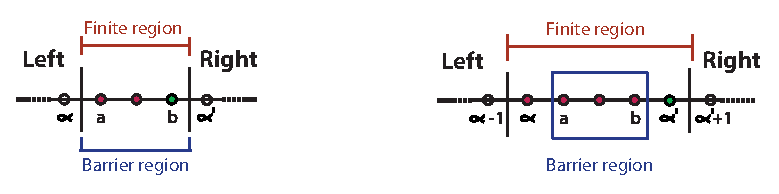
\includegraphics{fig2.eps}
\caption{(left) Representation of a three-layers structure where the finite region is identical to the barrier region. In this case the Rashba coupling term is defined at site $j = b$. (right) Representation of a three-layers structure where the finite region contains the barrier region and partially extends the left and right layers. In this case the Rashba coupling term is defined at site $j = \alp'$.}
\label{junction}
\end{figure}
%%%%%%%%%%%

Considering $t=-\frac{\hbar^2}{2ma^2}$ and $\eps =\frac{6\hbar^2}{2ma^2} + U(y)$, the Hamiltonian for each layer becomes,

\begin{align}
\h H_\Og &= \sum_{\substack{ijk \\ (ijkj \in \Og)}} \Bigg{\{} \eps_{ \Og,ijk} \bm{\h c}^{\dg}_{ijk} \bm{\h c}_{ijk} + \Dlt_\Og \Big{[}   \bm{\h c}^{\dg}_{ijk} \bm{\h \sg}\cdot\bm m\bm{\h c}_{ijk} \Big{]} \Bigg{\}}~~+ t\sum_{\substack{ijk \\ (ijk \in \Og)}}  \Big{[} \bm{\h c}^{\dg}_{i+1jk} \bm{\h c}_{ijk}+ \bm{\h c}^{\dg}_{ij+1k} \bm{\h c}_{ijk}+ \bm{\h c}^{\dg}_{ijk+1} \bm{\h c}_{ijk}  + h.c. \Big{]} \nn\\
&+\sum_{ik, j=b} \frac{\lambda_{so}}{2a} \Big{[} \big{(}i c_{i+1k}^{\dagger \uparrow} c_{ik}^\uparrow  - i c_{i+1k}^{\dagger \downarrow} c_{ik}^\downarrow + h.c. \big{)} +  \big{(} -i c_{ik+1}^{\dagger \downarrow}  c_{ik}^\uparrow  - i c_{ik+1}^{\dagger \uparrow}  c_{ik}^\downarrow + h.c. \big{)}  \Big{]},
\label{eq:wogo}
\end{align}


 where $\bm{\h c}^{\dg}_{j} =(\h c^{\dg \upa}_j,\h c^{\dg \dna}_j)$ and  $\bm{\h c}_{j} =(\h c^{\upa}_j,\h c^{\dna}_j)^t$. $t$ is the hopping matrix element, which couples the orbital states and therefore allows the electron to hop from one site to one of its neighbors and $\eps$ is the on-site energy. Notice that we are assuming a spin-independent hopping matrix element. For each layer we have,
 
 \begin{align}
\eps_L &= \frac{6\hbar^2}{2ma^2},  \\
\eps_B &= \frac{6\hbar^2}{2ma^2} + U(y), \\
\eps_R &= \frac{6\hbar^2}{2ma^2} 
\label{eq:wogoleft}
\end{align}
 
 Considering $\eps^{\upa(\dna)}=\eps \pm \Dlt $ the total on-site energy for majority (minority) carriers we define,
 
\begin{align}
 \label{avgeps}
  \eps^0 = \frac{\eps^\upa + \eps^\dna }{2}, \\
 \Dlt = \frac{ \eps^\upa - \eps^\dna}{2},
 \label{avgxc}
 \end{align}
 
 where $\eps^0$ is referred to as the averaged on-site energy. In the free-electron picture it is given by $\eps^0_{L(R)} = \frac{6\hbar^2}{2ma^2}$ in the electrodes and $\eps^0_B = \frac{6\hbar^2}{2ma^2} + U (y)$ in the barrier. $\Dlt$ is the usual exchange parameter that appears in Eq. \eqref{1qh}. Notice that $\Dlt$ is negative; therefore, $\eps^\upa$, associated with the spin-up electrons channel, is at a lower energy compared to $\eps^\dna$, associated with the spin-down electrons channel. To couple the barrier layer with the electrodes we consider the interaction Hamiltonian given in Eq. \eqref{eq:hamiltonian} and defined as
 
\begin{align}
\h H_{interaction}=t \Big{[} {\h c}_{a}^{\uparrow \dg}{\h c}_{\alp}^\uparrow + {\h c}_{a}^{\downarrow \dg}{\h c}_{\alp}^\downarrow + {\h c}_{b}^{\uparrow \dg}{\h c}_{\alp'}^\uparrow + {\h c}_{b}^{\downarrow \dg}{\h c}_{\alp'}^\downarrow + h.c. \Big{]}.
\label{eq:int}
\end{align}

Site $j=\alpha$ $(\alpha')$ in the left (right) electrode is next to site $j=a$ $(b)$ in the barrier region, see Fig. \ref{junction}.  In this same region, the potential energy varies linearly  with site number $j$, i.e.,

\begin{equation}
U_j = \mu_L +  (\mu_R - \mu_L) \frac{j-1}{N_B-1},
\label{eq:barepslinear}
\end{equation}

being $eV=\mu_R - \mu_L$ the potential drop, with $\mu_{L(R)}$ the chemical potential in the left (right) lead, and $N_B$ the number of atomic sites. Considering that transverse to $y-$axis, $\bm{k}=(k_x,k_y,k_z)$ is conserved then we can consider a solution of the form,

\begin{align}
\label{eq:bloch1}
\mid \psi_{k_x,k_z}^\sg \rangle &= \frac{1}{\sqrt{N_x}}\frac{1}{\sqrt{N_z}} \sum_{\substack{l\in x\\m\in z}} e^{ik_x a l}  e^{ik_z a m} \mid l,m, \sg \rangle, \\
\langle \psi_{k_x,k_z}^{\sg'} \mid &= \frac{1}{\sqrt{N_x}}\frac{1}{\sqrt{N_z}} \sum_{\substack{l'\in x\\m'\in z}} e^{-ik_x a l'}  e^{-ik_z a m'} \langle l',m', \sg' \mid. 
\label{eq:bloch2}
\end{align}

This is the usual Bloch wavefunction solution for a periodic potential in a tight binding model. $N_{x(z)}$ and l (m) represent the number of lattice points and site enumeration along x (z). If we consider in Eq. \eqref{eq:wogo}, $\h H_{{\bm k}_{||}}= t\sum_{ik}  \Big{[} \bm{\h c}^{\dg}_{i+1jk} \bm{\h c}_{ijk}+ \bm{\h c}^{\dg}_{ijk+1} \bm{\h c}_{ijk}  + h.c. \Big{]}$, then its matrix elements, in terms of Eqs. \eqref{eq:bloch1}-\eqref{eq:bloch2}, are

\begin{align}
\h H^{\sg,\sg'}_{{\bm k}_{||}}&=\langle \psi_{k_x,k_z}^{\sg'} \mid \h H_{{\bm k}_{||}} \mid \psi_{k_x,k_z}^\sg \rangle  \nn\\
&=\frac{1}{N_x N_z} \sum_{ll',mm'} e^{ik_x a(l-l')}e^{ik_z a(m-m')} \langle l',m',\sg' \mid \h H_{{\bm k}_{||}} \mid l,m \sg \rangle.
\label{matrixel}
\end{align}

To solve Eq. \eqref{matrixel} a simple cubic lattice in the nearest neighbor approximation is considered, then


\begin{align}
\h H^{\upa,\upa}_{{\bm k}_{||}} &= \frac{1}{N_x N_z} \sum_{ll',mm'} e^{ik_x a(l-l')}e^{ik_z a(m-m')} \langle l',m',\upa \mid t\sum_{ik} c_{i+1jk}^{\upa\dagger}c_{ijk}^{\upa} + c_{ijk+1}^{\upa\dg} c_{ijk}^{\upa} + c_{ijk}^{\upa\dg}c_{i+1jk}^{\upa} +  c_{ijk}^{\upa\dg} c_{ijk+1}^{\upa}   \mid l,m \upa \rangle \nn\\&=  \frac{1}{N_x N_z} \sum_{ll',mm'} e^{ik_x a(l-l')}e^{ik_z a(m-m')} t \langle l',m',\upa \mid  c_{l+1jm}^{\upa\dagger}c_{ljm}^{\upa} + c_{ljm+1}^{\upa\dg} c_{ljm}^{\upa} + c_{l-1jk}^{\upa\dg}c_{ljm}^{\upa} +  c_{ljm-1}^{\upa\dg} c_{ljm}^{\upa}   \mid l,m \upa \rangle \nn\\
&= \frac{1}{N_x N_z} \sum_{ll',mm'} e^{ik_x a(l-l')}e^{ik_z a(m-m')} t  \langle l',m',\upa \mid \big{(} \mid l+1,m \upa \rangle + \mid l,m+1 \upa \rangle + \mid l-1,m \upa \rangle + \mid l,m-1 \upa \rangle\big{)} \nn\\
&=  \frac{t}{N_x N_z} \sum_{l,mm'} e^{ik_x a}e^{ik_z a(m-m')}   \langle l-1,m',\upa \mid \big{(} \mid l+1,m \upa \rangle + \mid l,m+1 \upa \rangle + \mid l-1,m \upa \rangle + \mid l,m-1 \upa \rangle\big{)} \nn\\& ~~~~~~~~~~~~~~~~~+ e^{ik_z a(m-m')}   \langle l,m',\upa \mid \big{(} \mid l+1,m \upa \rangle + \mid l,m+1 \upa \rangle + \mid l-1,m \upa \rangle + \mid l,m-1 \upa \rangle\big{)} \nn\\&  ~~~~~~~~~~~~~~~~~+ e^{-ik_x a}e^{ik_z a(m-m')}   \langle l+1,m',\upa \mid \big{(} \mid l+1,m \upa \rangle + \mid l,m+1 \upa \rangle + \mid l-1,m \upa \rangle + \mid l,m-1 \upa \rangle\big{)} \nn\\
&=\frac{t}{N_x N_z} \sum_{l,mm'} e^{ik_x a}e^{ik_z a(m-m')}   \langle l-1,m',\upa \mid  l-1,m \upa \rangle  + e^{ik_z a(m-m')}   \langle l,m',\upa \mid \big{(}  \mid l,m+1 \upa \rangle  + \mid l,m-1 \upa \rangle\big{)} \nn\\&  ~~~~~~~~~~~~~~~~~+ e^{-ik_x a}e^{ik_z a(m-m')}   \langle l+1,m',\upa \mid l+1,m \upa \rangle \nn\\
&=\frac{t}{N_x N_z} \sum_{l,m} e^{ik_x a}     + e^{-ik_z a} +  e^{ik_z a}  + e^{-ik_x a} \nn\\
&= 2t(\cos k_xa + \cos k_z a).
\end{align}

It is easy to see that, $\h H^{\dna,\dna}_{{\bm k}_{||}} = \h H^{\upa,\upa}_{{\bm k}_{||}}$ and $\h H^{\upa,\dna (\dna,\upa)}_{{\bm k}_{||}} = 0$.
We define $\epsilon_{\bm k_\para} = 2t (\cos k_xa + \cos k_z a)$ as the in-plane energy and proceed to give a solution for the total wavefunction in each uncoupled region $\Og$ ($left$, $right$, or $finite$). 

%%%%%%%%%%%%%%%%%%%
%%%%%%%%%%%%%%%%%%%
\section{Green's function formalism}

We employ the Green's function formalism in Schrodinger's equation, i.e., $(E-H)\psi=0 \rightarrow (E-H)G=I$, where $G$ denotes the Green's function, $H$ is given in Eq. \eqref{eq:wogo}, and $E$ is the energy. 

%%%%%%%%%%%%%%%%%%%
%%%%%%%%%%%%%%%%%%%
\subsection{Isolated Green's functions in the finite region}
In previous sections we derived a second quantization Free-electron representation of the Hamiltonian. Here we directly present the tight binding model. Following Kalitsov's paper,\cite{kalitsov} the one electron Schrodinger equation for the spin dependent retarded Green's function $g_{pq}$ for each uncoupled region reads,

\begin{equation}
\sum_{p_1} \Bigg \{ \bigg\{ [(E-\eps_{\bm{k}_{||}})\dlt_{pp_1}-\overline{H}_{pp_1}]\hat{I}-\dlt H_{p,p_1} \bigg[\begin{array}{ccc}\cos\theta_\Og & \sin\theta_\Og e^{-i\phi_\Og} \\
\sin\theta_\Og e^{i\phi_\Og} & -\cos\theta_\Og 
 \end{array} \bigg] -  \bar{\lambda}_{R} \left(\begin{array}{cc} 
2\sin k_xa  &  -2\sin k_za\\
-2\sin k_za &  -2\sin k_xa
\end{array}\right) \bigg \} \left(\begin{array}{cc} \hat{g}^{\upa\upa}_{p_1q}  &  \hat{g}^{\upa\dna}_{p_1q} \\  \hat{g}^{\dna\upa}_{p_1q} &  \hat{g}^{\dna\dna}_{p_1q} \end{array}\right)  \Bigg \}=\dlt_{pq}\hat{I}.
 \label{tbschrodinger}
\end{equation}

$p_1$, $p$, and $q$ denote atomic sites along $y-$axis. ${\hat I}$ is the 2$\times$2 unit matrix operator, and $\theta_\Og$ is the angle of the magnetization with respect to the $z-$axis. $\overline{H}_{pq} = \eps^0_\Og\dlt_{pq} + t(\dlt_{p,q+1}+\dlt_{p,q-1})$ and $\dlt H_{pq}= \Dlt_\Og \dlt_{pq}$, where $\eps^0$ and $\Dlt$ are defined in Eqs. \eqref{avgeps}-\eqref{avgxc}.
The last term is the Rashba coupling in the nearest neighbor approximation, where we considered $\bm k$ to be conserved transverse to $y$. In what follows, we will derive the case where the Rashba coupling term is defined at $j=b$, then $\bar{\lam}_R = \frac{\lam_{so}}{2a}\dlt_{p_1b}$. For the case where it is given at $j=\alp'$ (right panel in Fig. \ref{junction}), the solution is directly given in the Fortran code.
Notice that conservation of ${\bf k}_\para = (k_x,k_z)$ allows us to reduce our problem to a pseudo-one dimensional system. We now proceed to solve the one-electron Schrodinger equation for the spin dependent retarded Green's function in the finite region. To ease the discussion we start from the most simple scenario: a finite region given by a barrier of 3 sites.

%%%%%%%%%%%%%%%%
\subsubsection{Finite Region: 3-sites Barrier}
 For the particular case of a finite region given by a barrier of 3 sites, Eq. \eqref{tbschrodinger} in its matrix form is given by,


\begin{align}
 \left[ \left(\begin{array}{ccc} 
E    &  0 & 0 \\
0 &  E & 0 \\
 0 & 0 & E
\end{array}\right) -
 \left(\begin{array}{ccc} 
h_1   &  t & 0 \\
t &  h_2 & t \\
 0 & t & h_3
\end{array}\right) \right] 
 \left(\begin{array}{ccc} 
g_{11}   &  g_{12} & g_{13} \\
g_{21} &  g_{22} & g_{23} \\
g_{31} & g_{32} & g_{33} 
\end{array}\right) =  
 \left(\begin{array}{ccc} 
 1   &  0 & 0 \\
0 &  1 & 0 \\
 0 & 0 & 1 
\end{array}\right). 
\label{mat}
\end{align}

In general  each element in Eq. \eqref{mat} has 4 components in spin space. $h_3$ is of particular interest as it contains the Rashba coupling term $(j=b)$. We have,

\begin{widetext}
\begin{align}
h1 &=\left(\begin{array}{cc} 
\eps^0 + \mu_L +2t \sum_{l}\cos k_la &  0\\
0 &  \eps^0 + \mu_L +2t \sum_{l}\cos k_la
\end{array}\right) +\Dlt \left(\begin{array}{cc} 
\cos\theta  &  \sin\theta e^{-i\phi}\\
\sin\theta e^{i\phi} &  -\cos\theta
\end{array}\right),\\
h2 &=\left(\begin{array}{cc} 
(\eps^0 + \frac{\mu_R + \mu_L}{2}) +2t \sum_{l}\cos k_la &  0\\
0 &  (\eps^0 + \frac{\mu_R + \mu_L}{2}) +2t \sum_{l}\cos k_la
\end{array}\right)+\Dlt \left(\begin{array}{cc} 
\cos\theta  &  \sin\theta e^{-i\phi}\\
\sin\theta e^{i\phi} &  -\cos\theta
\end{array}\right),\\
h3 &=\left(\begin{array}{cc} 
(\eps^0 +\mu_R) +2t \sum_{l}\cos k_la &  0\\
0 &  (\eps^0 + \mu_R) +2t \sum_{l}\cos k_la
\end{array}\right) +\Dlt \left(\begin{array}{cc} 
\cos\theta  &  \sin\theta e^{-i\phi}\\
\sin\theta e^{i\phi} &  -\cos\theta
\end{array}\right)
+\lambda_{R} \left(\begin{array}{cc} 
2\sin k_xa  &  -2\sin k_za\\
-2\sin k_za &  -2\sin k_xa
\end{array}\right),
\label{mat2}
\end{align}
\end{widetext}

where $l=x,z$. If $\Dlt=0$ then the system is non-magnetic. Notice that we have dropped out subindex $B$ for simplicity. In its extended form, Eq. \eqref{mat} is expressed as,

\begin{align}
\left[ \left(\begin{array}{cccccc} 
 E   &  0 & 0 &  0 & 0 &  0  \\
0 &  E & 0 & 0 &  0 & 0 \\
 0 & 0 & E & 0 &  0 & 0 \\
 0 & 0 & 0 & E &  0 & 0 \\
  0 & 0 & 0 & 0 &  E & 0 \\
   0 & 0 & 0 & 0 &  0 & E
\end{array}\right) -
 \left(\begin{array}{cccccc} 
h_{11}^{\upa\upa}   &  h_{11}^{\upa\dna} & h_{12}^{\upa\upa} & h_{12}^{\upa\dna} &   h_{13}^{\upa\upa} & h_{13}^{\upa\dna}\\
h_{11}^{\dna\upa}   &  h_{11}^{\dna\dna} & h_{12}^{\dna\upa} & h_{12}^{\dna\dna} &   h_{13}^{\dna\upa} & h_{13}^{\dna\dna}\\
h_{21}^{\upa\upa}   &  h_{21}^{\upa\dna} & h_{22}^{\upa\upa} & h_{22}^{\upa\dna} &   h_{23}^{\upa\upa} & h_{23}^{\upa\dna} \\
h_{21}^{\dna\upa}   &  h_{21}^{\dna\dna} & h_{22}^{\dna\upa} & h_{22}^{\dna\dna} &   h_{23}^{\dna\upa} & h_{23}^{\dna\dna} \\
h_{31}^{\upa\upa}   &  h_{31}^{\upa\dna} & h_{32}^{\upa\upa} & h_{32}^{\upa\dna} &   h_{33}^{\upa\upa} & h_{33}^{\upa\dna} \\
h_{31}^{\dna\upa}   &  h_{31}^{\dna\dna} & h_{32}^{\dna\upa} & h_{32}^{\dna\dna} &   h_{33}^{\dna\upa} & h_{33}^{\dna\dna} \\
\end{array}\right) \right]
 \left(\begin{array}{cccccc} 
g_{11}^{\upa\upa}   &  g_{11}^{\upa\dna} & g_{12}^{\upa\upa}   &  g_{12}^{\upa\dna} & g_{13}^{\upa\upa}   &  g_{13}^{\upa\dna} \\
g_{11}^{\dna\upa} &  g_{11}^{\dna\dna}& g_{12}^{\dna\upa}   &  g_{12}^{\dna\dna} & g_{13}^{\dna\upa}   &  g_{13}^{\dna\dna} \\
g_{21}^{\upa\upa}   &  g_{21}^{\upa\dna} & g_{22}^{\upa\upa}   &  g_{22}^{\upa\dna} & g_{23}^{\upa\upa}   &  g_{23}^{\upa\dna} \\
g_{21}^{\dna\upa} &  g_{21}^{\dna\dna}& g_{22}^{\dna\upa}   &  g_{22}^{\dna\dna} & g_{23}^{\dna\upa}   &  g_{23}^{\dna\dna} \\
g_{31}^{\upa\upa}   &  g_{31}^{\upa\dna} & g_{32}^{\upa\upa}   &  g_{32}^{\upa\dna} & g_{33}^{\upa\upa}   &  g_{33}^{\upa\dna} \\
g_{31}^{\dna\upa} &  g_{31}^{\dna\dna}& g_{32}^{\dna\upa}   &  g_{32}^{\dna\dna} & g_{33}^{\dna\upa}   &  g_{33}^{\dna\dna} 
\end{array}\right)  =  
 \left(\begin{array}{cccccc} 
 1   &  0 & 0 &  0 & 0 &  0  \\
0 &  1 & 0 & 0 &  0 & 0 \\
 0 & 0 & 1 & 0 &  0 & 0 \\
 0 & 0 & 0 & 1 &  0 & 0 \\
  0 & 0 & 0 & 0 &  1 & 0 \\
   0 & 0 & 0 & 0 &  0 & 1,
\end{array}\right). 
\label{mat001}
\end{align}


where $h_{j,j\pm1}^{\upa\upa(\dna\dna)}$ = t, $h_{j,j\pm1}^{\upa\dna(\dna\upa)}=0$ and  $h_{j,j\pm2}^{\upa\upa(\dna\dna)}$ = $h_{j,j\pm2}^{\upa\dna(\dna\upa)}$ = 0. Notice that reordering the expression won't affect the matrix; therefore we have,

\begin{align}
\left[ \left(\begin{array}{cccccc} 
 E   &  0 & 0 &  0 & 0 &  0  \\
0 &  0 & 0 & E &  0 & 0 \\
 0 & E & 0 & 0 &  0 & 0 \\
 0 & 0 & 0 & 0 &  E & 0 \\
  0 & 0 & E & 0 &  0 & 0 \\
   0 & 0 & 0 & 0 &  0 & E
\end{array}\right) -
 \left(\begin{array}{cccccc} 
h_{11}^{\upa\upa}   & h_{12}^{\upa\upa} &   h_{13}^{\upa\upa} &  h_{11}^{\upa\dna}  & h_{12}^{\upa\dna}  & h_{13}^{\upa\dna}\\
h_{11}^{\dna\upa}   & h_{12}^{\dna\upa} &   h_{13}^{\dna\upa} &  h_{11}^{\dna\dna}  & h_{12}^{\dna\dna}  & h_{13}^{\dna\dna}\\
h_{21}^{\upa\upa}   & h_{22}^{\upa\upa} &   h_{23}^{\upa\upa} &  h_{21}^{\upa\dna}  & h_{22}^{\upa\dna}  & h_{23}^{\upa\dna} \\
h_{21}^{\dna\upa}   & h_{22}^{\dna\upa} &   h_{23}^{\dna\upa} &  h_{21}^{\dna\dna}  & h_{22}^{\dna\dna}  & h_{23}^{\dna\dna} \\
h_{31}^{\upa\upa}   & h_{32}^{\upa\upa} &   h_{33}^{\upa\upa}  &  h_{31}^{\upa\dna}  & h_{32}^{\upa\dna} & h_{33}^{\upa\dna} \\
h_{31}^{\dna\upa}   & h_{32}^{\dna\upa} &   h_{33}^{\dna\upa} &  h_{31}^{\dna\dna}  & h_{32}^{\dna\dna}  & h_{33}^{\dna\dna} \\
\end{array}\right) \right]
 \left(\begin{array}{cccccc} 
g_{11}^{\upa\upa}  & g_{12}^{\upa\upa}  & g_{13}^{\upa\upa} &  g_{11}^{\upa\dna}   &  g_{12}^{\upa\dna}    &  g_{13}^{\upa\dna} \\
g_{11}^{\dna\upa} & g_{12}^{\dna\upa} & g_{13}^{\dna\upa} &  g_{11}^{\dna\dna}  &  g_{12}^{\dna\dna}    &  g_{13}^{\dna\dna} \\
g_{21}^{\upa\upa}   & g_{22}^{\upa\upa} & g_{23}^{\upa\upa}  &  g_{21}^{\upa\dna}    &  g_{22}^{\upa\dna}   &  g_{23}^{\upa\dna} \\
g_{21}^{\dna\upa} & g_{22}^{\dna\upa}  & g_{23}^{\dna\upa} &  g_{21}^{\dna\dna}  &  g_{22}^{\dna\dna}    &  g_{23}^{\dna\dna} \\
g_{31}^{\upa\upa}  & g_{32}^{\upa\upa}  & g_{33}^{\upa\upa}  &  g_{31}^{\upa\dna}    &  g_{32}^{\upa\dna}   &  g_{33}^{\upa\dna} \\
g_{31}^{\dna\upa} & g_{32}^{\dna\upa} & g_{33}^{\dna\upa} &  g_{31}^{\dna\dna}   &  g_{32}^{\dna\dna}    &  g_{33}^{\dna\dna} 
\end{array}\right)  =  
 \left(\begin{array}{cccccc} 
 1   &  0 & 0 &  0 & 0 &  0  \\
0 &  0 & 0 & 1 &  0 & 0 \\
 0 & 1 & 0 & 0 &  0 & 0 \\
 0 & 0 & 0 & 0 &  1 & 0 \\
  0 & 0 & 1 & 0 &  0 & 0 \\
   0 & 0 & 0 & 0 &  0 & 1,
\end{array}\right). 
\label{mat002}
\end{align}
 
 where we have interchanged in Eq. \eqref{mat001} column 3 with column 2, then column 5 with column 4, and last, column 4 with column 3. Similarly interchanging the rows in Eq. \eqref{mat002} we have,
 
 \begin{align}
\left[ \left(\begin{array}{cccccc} 
 E   &  0 & 0 &  0 & 0 &  0  \\
0 & E & 0 & 0 &  0 & 0 \\
  0 & 0 & E & 0 &  0 & 0 \\
0 &  0 & 0 & E &  0 & 0 \\
 0 & 0 & 0 & 0 &  E & 0 \\
   0 & 0 & 0 & 0 &  0 & E
\end{array}\right) -
 \left(\begin{array}{cccccc} 
h_{11}^{\upa\upa}   & h_{12}^{\upa\upa} &   h_{13}^{\upa\upa} &  h_{11}^{\upa\dna}  & h_{12}^{\upa\dna}  & h_{13}^{\upa\dna}\\
h_{21}^{\upa\upa}   & h_{22}^{\upa\upa} &   h_{23}^{\upa\upa} &  h_{21}^{\upa\dna}  & h_{22}^{\upa\dna}  & h_{23}^{\upa\dna} \\
h_{31}^{\upa\upa}   & h_{32}^{\upa\upa} &   h_{33}^{\upa\upa}  &  h_{31}^{\upa\dna}  & h_{32}^{\upa\dna} & h_{33}^{\upa\dna} \\
h_{11}^{\dna\upa}   & h_{12}^{\dna\upa} &   h_{13}^{\dna\upa} &  h_{11}^{\dna\dna}  & h_{12}^{\dna\dna}  & h_{13}^{\dna\dna}\\
h_{21}^{\dna\upa}   & h_{22}^{\dna\upa} &   h_{23}^{\dna\upa} &  h_{21}^{\dna\dna}  & h_{22}^{\dna\dna}  & h_{23}^{\dna\dna} \\
h_{31}^{\dna\upa}   & h_{32}^{\dna\upa} &   h_{33}^{\dna\upa} &  h_{31}^{\dna\dna}  & h_{32}^{\dna\dna}  & h_{33}^{\dna\dna} \\
\end{array}\right) \right]
 \left(\begin{array}{cccccc} 
g_{11}^{\upa\upa}  & g_{12}^{\upa\upa}  & g_{13}^{\upa\upa} &  g_{11}^{\upa\dna}   &  g_{12}^{\upa\dna}    &  g_{13}^{\upa\dna} \\
g_{21}^{\upa\upa}   & g_{22}^{\upa\upa} & g_{23}^{\upa\upa}  &  g_{21}^{\upa\dna}    &  g_{22}^{\upa\dna}   &  g_{23}^{\upa\dna} \\
g_{31}^{\upa\upa}  & g_{32}^{\upa\upa}  & g_{33}^{\upa\upa}  &  g_{31}^{\upa\dna}    &  g_{32}^{\upa\dna}   &  g_{33}^{\upa\dna} \\
g_{11}^{\dna\upa} & g_{12}^{\dna\upa} & g_{13}^{\dna\upa} &  g_{11}^{\dna\dna}  &  g_{12}^{\dna\dna}    &  g_{13}^{\dna\dna} \\
g_{21}^{\dna\upa} & g_{22}^{\dna\upa}  & g_{23}^{\dna\upa} &  g_{21}^{\dna\dna}  &  g_{22}^{\dna\dna}    &  g_{23}^{\dna\dna} \\
g_{31}^{\dna\upa} & g_{32}^{\dna\upa} & g_{33}^{\dna\upa} &  g_{31}^{\dna\dna}   &  g_{32}^{\dna\dna}    &  g_{33}^{\dna\dna} 
\end{array}\right)  =  
 \left(\begin{array}{cccccc} 
 1   &  0 & 0 &  0 & 0 &  0  \\
 0 & 1 & 0 & 0 &  0 & 0 \\
 0 & 0 & 1 & 0 &  0 & 0 \\
0 &  0 & 0 & 1 &  0 & 0 \\
0 & 0 & 0 & 0 &  1 & 0 \\
   0 & 0 & 0 & 0 &  0 & 1,
\end{array}\right). 
\label{mat003}
\end{align}

where row 3 was interchanged with row 2, then row 5 with row 4, and last, row 4 with row 3. This procedure can be extended to a $N\times N$ matrix. 

%%%%%%%%%%%%%%%%%%%%%%%
\subsubsection{Finite Region: 3-sites Barrier and 2-sites finite electrodes}
In a more general form, the finite region may extend to the electrodes (see right panel in Fig.  \ref{junction}). In this case we can consider the total number of sites in the finite region $N_F = N_L + N_B + N_R$. In this scenario the total number of sites for the electrodes is $N_{left (right)} + N_{L (R)}$, where the former is semi-infinite and the latter finite. The reason behind this approach is that we can include different layers with different properties in the finite region. As an example let's consider $N_L =2$, $N_B = 3$, and $N_R=2$ , then our matrix for the finite region becomes,

\begin{align}
 \left[ \left(\begin{array}{ccccccc} 
E    &  0 & 0 &  0 & 0 &  0 & 0 \\
0    &  E & 0 &  0 & 0 &  0 & 0 \\
0    & 0  & E &  0 & 0 &  0 & 0 \\
0    & 0  & 0 &  E & 0 &  0 & 0 \\
0    & 0  & 0 &  0 & E &  0 & 0 \\
0    & 0  & 0 &  0 & 0 &  E & 0 \\
0    & 0  & 0 &  0 & 0 &  0 & E 
\end{array}\right) -
 \left(\begin{array}{ccccccc} 
h_{1,L}   &  t & 0 & 0 & 0 & 0 & 0 \\
t &  h_{2,L} & t  & 0 & 0 & 0 & 0\\
 0 & t & h_{3,B} & t & 0 & 0 & 0 \\
  0 & 0 & t & h_{4,B} & t & 0 & 0 \\
  0 & 0 & 0 & t & h_{5,B} & t & 0 \\
  0 & 0 & 0 & 0 & t & h_{6,R} & t \\
  0 & 0 & 0 &0 & 0 & t & h_{7,R} \\
\end{array}\right) \right] 
 \left(\begin{array}{ccccccc} 
g_{11}   &  g_{12} & g_{13} & g_{14}   &  g_{15} & g_{16} & g_{17}  \\
g_{21}   &  g_{22} & g_{23} & g_{24}   &  g_{25} & g_{26} & g_{17}  \\
g_{31}   &  g_{32} & g_{33} & g_{34}   &  g_{35} & g_{36} & g_{37}  \\
g_{41}   &  g_{42} & g_{43} & g_{44}   &  g_{45} & g_{46} & g_{47}  \\
g_{51}   &  g_{52} & g_{53} & g_{54}   &  g_{55} & g_{56} & g_{57}  \\
g_{61}   &  g_{62} & g_{63} & g_{64}   &  g_{65} & g_{66} & g_{67}  \\
g_{71}   &  g_{72} & g_{73} & g_{74}   &  g_{75} & g_{76} & g_{77}  
\end{array}\right) =  
I,
\label{mat004}
\end{align}

where again each term has four components in spin space. Similarly, by matrix reordering we have,

\begin{align}
 \left[ \left(\begin{array}{cccccc} 
E    &  0 & 0 &  0 & ... &  0  \\
0    &  E & 0 &  0 & 0 &  ...  \\
0    & 0  & ... &  0 & 0 &  0  \\
0    & 0  & 0 &  ... & 0 &  0  \\
...    & 0  & 0 &  0 & E &  0  \\
0    & ...  & 0 &  0 & 0 &  E 
\end{array}\right) -
 \left(\begin{array}{cccccc} 
h^{\upa\upa}_{11}   &  ... & h^{\upa\upa}_{17} & h^{\upa\dna}_{11}  & ... & h^{\upa\dna}_{17}   \\
... &  ... & ...  & ... & ... & ... \\
 h^{\upa\upa}_{71} & ... &  h^{\upa\upa}_{77} &  h^{\upa\dna}_{71} & ... & h^{\upa\dna}_{77}   \\
  h^{\dna\upa}_{11} & ... & h^{\dna\upa}_{17} & h^{\dna\dna}_{11} & ... & h^{\dna\dna}_{17}  \\
... &  ... & ...  & ... & ... & ...  \\
h^{\dna\upa}_{71} & ... &  h^{\dna\upa}_{77} &  h^{\dna\dna}_{71} & ... & h^{\dna\dna}_{77}  
\end{array}\right) \right] 
 \left(\begin{array}{ccccccc} 
g^{\upa\upa}_{11}   &  ... & g^{\upa\upa}_{17} & g^{\upa\dna}_{11}  & ... & g^{\upa\dna}_{17}   \\
... &  ... & ...  & ... & ... & ... \\
 g^{\upa\upa}_{71} & ... &  g^{\upa\upa}_{77} &  g^{\upa\dna}_{71} & ... & g^{\upa\dna}_{77}   \\
  g^{\dna\upa}_{11} & ... & g^{\dna\upa}_{17} & g^{\dna\dna}_{11} & ... & g^{\dna\dna}_{17}  \\
... &  ... & ...  & ... & ... & ...  \\
g^{\dna\upa}_{71} & ... &  g^{\dna\upa}_{77} &  g^{\dna\dna}_{71} & ... & g^{\dna\dna}_{77}  \end{array}\right) =  
I.
\label{mat005}
\end{align}

To ease the discussion we change the notation of the above expression to

\begin{align}
 \left[ \left(\begin{array}{cccccc} 
E    &  0 & 0 &  0 & ... &  0  \\
0    &  E & 0 &  0 & 0 &  ...  \\
0    & 0  & ... &  0 & 0 &  0  \\
0    & 0  & 0 &  ... & 0 &  0  \\
...    & 0  & 0 &  0 & E &  0  \\
0    & ...  & 0 &  0 & 0 &  E 
\end{array}\right) -
 \left(\begin{array}{cccccc} 
h_{1,1}   &  ... & h_{1,7} & h_{1,8}  & ... &h_{1,14}   \\
... &  ... & ...  & ... & ... & ... \\
 h_{7,1} & ... &  h_{7,7} &  h_{7,8} & ... & h_{7,14}   \\
  h_{8,1} & ... & h_{8,7} & h_{8,8} & ... & h_{8,14}  \\
... &  ... & ...  & ... & ... & ...  \\
h_{14,1} & ... &  h_{14,7} &  h_{14,8} & ... & h_{14,14}  
\end{array}\right) \right] 
 \left(\begin{array}{ccccccc} 
g_{1,1}   &  ... & g_{1,7} & g_{1,8}  & ... & g_{1,14}   \\
... &  ... & ...  & ... & ... & ... \\
 g_{7,1} & ... &  g_{7,7} &  g_{7,8} & ... & g_{7,14}   \\
  g_{8,1} & ... & g_{8,7} & g_{8,8} & ... & g_{8,14}  \\
... &  ... & ...  & ... & ... & ...  \\
g_{14,1} & ... &  g_{14,7} &  g_{14,8} & ... & g_{14,14}  \end{array}\right) =  
I,
\label{mat006}
\end{align}


where, e.g., $h_{1,8}\equiv h^{\upa\dna}_{11} $ and $ h_{14,14}  =h^{\dna\dna}_{77}.$ Eq. \eqref{mat006} notation is used in the following.

%%%%%%%%%%%%%%%%%%%%%%%%%%%%%%%%%%%
\subsubsection{Finite Region: Barrier and finite electrodes with general number of sites}

Considering $N_L$ to be finite, then the L-region is given by,


\begin{align}
h_{j,j}&= \eps^0_L + \mu_L + 2t(\cos k_x a + \cos k_z a) + \Dlt_L \cos\theta_L, \\
h_{N_L+N_B+N_R+j,N_L+N_B+N_R+j} &= \eps^0_L + \mu_L + 2t(\cos k_x a + \cos k_z a) - \Dlt_L \cos\theta_L, \\
h_{j, N_L+N_B+N_R+j} &= \Dlt_L \sin\theta_L e^{-i\phi_L } = \Dlt_L  (\sin\theta_L\cos\phi_L - i\sin\theta_L\sin\phi_L) \\
h_{N_L+N_B+N_R+j, j} &= \Dlt_L \sin\theta_L e^{i\phi_L }~~ = \Dlt_L  (\sin\theta_L\cos\phi_L + i\sin\theta_L\sin\phi_L) 
\end{align}

where $j$ runs from $j=1$ to j=$N_L$ and $U_j$ is given in Eq. \eqref{eq:barepslinear}.  For the barrier region (B-region) we have,

\begin{align}
h_{N_L+j, N_L+j}&= \eps^0_B + U_j  + 2t(\cos k_x a + \cos k_z a) + \Dlt_B \cos\theta_B, \\
h_{2N_L+N_B+N_R+j,2N_L+N_B+N_R+j} &= \eps^0_B  + U_j  + 2t(\cos k_x a + \cos k_z a) - \Dlt_B \cos\theta_B, \\
h_{N_L+j, 2N_L+N_B+N_R+j} &= \Dlt_B \sin\theta_B e^{-i\phi_B } = \Dlt_B  (\sin\theta_B\cos\phi_B - i\sin\theta_B\sin\phi_B), \\
h_{2N_L+N_B+N_R+j, N_L+j} &= \Dlt_B \sin\theta_B e^{i\phi_B }~~ = \Dlt_B  (\sin\theta_B\cos\phi_B + i\sin\theta_B\sin\phi_B), 
\end{align}

where j runs from $1$ to $N_B-1$. For $j=N_B$ we have,

\begin{align}
h_{N_L+N_B, N_L+N_B}&= \eps^0_B + U(N_B)  + 2t(\cos k_x a + \cos k_z a) + \Dlt_B \cos\theta_B + 2\lam_R \sin k_x a, \\
h_{2N_L+2N_B+N_R,2N_L+2N_B+N_R} &= \eps^0_B  + U(N_B)  + 2t(\cos k_x a + \cos k_z a) - \Dlt_B \cos\theta_B -  2\lam_R \sin k_x a,\\
h_{N_L+N_B, 2N_L+2N_B+N_R} &=  \Dlt_B  (\sin\theta_B\cos\phi_B - i\sin\theta_B\sin\phi_B) -  2\lam_R \sin k_z a, \\
h_{2N_L+2N_B+N_R, N_L+N_B} &=  \Dlt_B  (\sin\theta_B\cos\phi_B + i\sin\theta_B\sin\phi_B) -  2\lam_R \sin k_z a. 
\end{align}

As seen, the Rashba coupling term is defined at $j=b$ only. Considering $N_R$ to be finite, then the $R-$region is given by,

\begin{align}
h_{N_L+N_B+j, N_L + N_B + j}&= \eps^0_R + \mu_R + 2t(\cos k_x a + \cos k_z a) + \Dlt_R \cos\theta_R, \\
h_{2N_L+2N_B+N_R+j,2N_L+2N_B+N_R+j} &= \eps^0_R + \mu_R + 2t(\cos k_x a + \cos k_z a) - \Dlt_R \cos\theta_R, \\
h_{N_L + N_B + j, 2N_L+2N_B+N_R+j} &= \Dlt_R \sin\theta_R e^{-i\phi_R } = \Dlt_R  (\sin\theta_R\cos\phi_R - i\sin\theta_R\sin\phi_R), \\
h_{2N_L+2N_B+N_R+j, N_L+N_B+j} &= \Dlt_R \sin\theta_R e^{i\phi_R }~~ = \Dlt_R  (\sin\theta_R\cos\phi_R + i\sin\theta_R\sin\phi_R), 
\end{align}

where j goes from 1 to $N_R$. Finally the hopping terms are given by,

\begin{align}
h_{j,j+1} &= t, \\
h_{j+1, j} &= t, \\
h_{N_L+N_B+N_R+j, N_L+N_B+N_R+1+j} &= t, \\
h_{N_L+N_B+N_R+1+j, N_L+N_B+N_R + j} &= t.
\end{align}


To consider the retarded Green's functions, we take $E \rightarrow E + i\dlt$ and solve the system given in Eq. \eqref{mat006} by matrix inversion. This procedure is done numerically.

%%%%%%%%%%%%%%%%%%%%%%%
%%%%%%%%%%%%%%%%%%%%%%%
\subsection{Isolated Green's functions in the semi-infinite regions}


To obtain solutions for the isolated Green's functions in the semi-infinite electrodes we directly solve Eq. \eqref{tbschrodinger}, which turns into a system of 4 equations ($\h g_{pq}^{\uparrow\uparrow}$, $\h g_{pq}^{\uparrow\downarrow}$, $\h g_{pq}^{\downarrow\uparrow}$, and $\h g_{pq}^{\downarrow\downarrow}$). We have,

\begin{equation}
\sum_{p_1} \Bigg \{ \bigg[\begin{array}{ccc} (E-\eps_{\bm{k}_{||}})\dlt_{pp_1} -\overline{H}_{pp_1}  -\dlt H_{p,p_1} \cos\theta_\Og & -\dlt H_{p,p_1} \sin\theta_\Og e^{-i\phi_\Og} \\
-\dlt H_{p,p_1} \sin\theta_\Og e^{i\phi_\Og} & (E-\eps_{\bm{k}_{||}})\dlt_{pp_1} -\overline{H}_{pp_1}  +\dlt H_{p,p_1} \cos\theta_\Og 
 \end{array} \bigg]   \left(\begin{array}{cc} \hat{g}^{\upa\upa}_{p_1q}  &  \hat{g}^{\upa\dna}_{p_1q} \\  \hat{g}^{\dna\upa}_{p_1q} &  \hat{g}^{\dna\dna}_{p_1q} \end{array}\right)  \Bigg \}=\dlt_{pq}\hat{I},
 \label{tbschrodinger2}
\end{equation}

where each term reads,

\begin{align}
\label{line1}
\sum_{p_1} \Bigg \{ (E\dlt_{pp_1}-\eps_{\bm{k}_{||}}\dlt_{pp_1} -\overline{H}_{pp_1}  -\dlt H_{p,p_1} \cos\theta_\Og) \hat{g}^{\upa\upa}_{p_1q} -\dlt H_{p,p_1} \sin\theta_\Og e^{-i\phi_\Og}  \hat{g}^{\dna\upa}_{p_1q} \Bigg \}&=\dlt_{pq}, \\
\label{line2}
\sum_{p_1} \Bigg \{ (E\dlt_{pp_1}-\eps_{\bm{k}_{||}}\dlt_{pp_1} -\overline{H}_{pp_1}  -\dlt H_{p,p_1} \cos\theta_\Og) \hat{g}^{\upa\dna}_{p_1q} -\dlt H_{p,p_1} \sin\theta_\Og e^{-i\phi_\Og}  \hat{g}^{\dna\dna}_{p_1q} \Bigg \}&=0, \\
\label{line3}
\sum_{p_1} \Bigg \{ (E\dlt_{pp_1}-\eps_{\bm{k}_{||}}\dlt_{pp_1} -\overline{H}_{pp_1}  +\dlt H_{p,p_1} \cos\theta_\Og) \hat{g}^{\dna\upa}_{p_1q} -\dlt H_{p,p_1} \sin\theta_\Og e^{i\phi_\Og}  \hat{g}^{\upa\upa}_{p_1q} \Bigg \}&=0, \\
\sum_{p_1} \Bigg \{ (E\dlt_{pp_1}-\eps_{\bm{k}_{||}}\dlt_{pp_1} -\overline{H}_{pp_1}  +\dlt H_{p,p_1} \cos\theta_\Og) \hat{g}^{\dna\dna}_{p_1q} -\dlt H_{p,p_1} \sin\theta_\Og e^{i\phi_\Og}  \hat{g}^{\upa\dna}_{p_1q} \Bigg \}&=\dlt_{pq}, 
 \label{line4}
\end{align}

Recall that $\overline H_{pp_1} = \eps^0_\Og \dlt_{pp_1} + t(\dlt_{p,p_1+1} + \dlt_{p,p_1-1})$ and $\dlt H_{pp_1} = \Dlt_\Og \dlt_{pp_1}$.
Considering nearest neighbours, i.e., $\h g_{p+1,q} = \h g_{pq}e^{ik_ya}$ and $\h g_{p-1,q} = \h g_{pq}e^{-ik_ya}$, Eq. \eqref{line1} reduces to, 

\begin{align}
(E-\eps_{\bm{k}_{||}})\hat{g}^{\upa\upa}_{pq} + \sum_{p_1} \Bigg \{ ( -\overline{H}_{pp_1}  -\dlt H_{p,p_1} \cos\theta_\Og) \hat{g}^{\upa\upa}_{p_1q} -\dlt H_{p,p_1} \sin\theta_\Og e^{-i\phi_\Og}  \hat{g}^{\dna\upa}_{p_1q} \Bigg \}&=\dlt_{pq}, \nn\\
(E-\eps_{\bm{k}_{||}})\hat{g}^{\upa\upa}_{pq} - \eps_\Og^0 \hat{g}^{\upa\upa}_{pq}  -t \hat{g}^{\upa\upa}_{p-1,q} -t \hat{g}^{\upa\upa}_{p+1,q}  -\Dlt_\Og \cos\theta_\Og \hat{g}^{\upa\upa}_{pq} -\Dlt_\Og \sin\theta_\Og e^{-i\phi_\Og}  \hat{g}^{\dna\upa}_{pq} &=\dlt_{pq}, \nn\\
(E-\eps_{\bm{k}_{||}})\hat{g}^{\upa\upa}_{pq} - \eps_\Og^0 \hat{g}^{\upa\upa}_{pq}  -t \hat{g}^{\upa\upa}_{p,q}e^{-ik_ya} -t \hat{g}^{\upa\upa}_{p,q}e^{ik_ya}  -\Dlt_\Og \cos\theta_\Og \hat{g}^{\upa\upa}_{pq} -\Dlt_\Og \sin\theta_\Og e^{-i\phi_\Og}  \hat{g}^{\dna\upa}_{pq} &=\dlt_{pq}, \nn\\
(E-\eps_{\bm{k}_{||}}- \eps_\Og^0   -2t\cos k_ya  -\Dlt_\Og \cos\theta_\Og) \hat{g}^{\upa\upa}_{pq} -\Dlt_\Og \sin\theta_\Og e^{-i\phi_\Og}  \hat{g}^{\dna\upa}_{pq} &=\dlt_{pq}.
 \label{tbschrodinger41}
\end{align}

A similar approach is taken for Eqs. \eqref{line2}-\eqref{line4}; therefore, we have

\begin{align}
\label{lineg0}
(E-\eps_{\bm{k}_{||}}- \eps_\Og^0   -2t\cos k_ya  -\Dlt_\Og \cos\theta_\Og) \hat{g}^{\upa\upa}_{pq} -\Dlt_\Og \sin\theta_\Og e^{-i\phi_\Og}  \hat{g}^{\dna\upa}_{pq} &=\dlt_{pq}, \\
\label{lineg1}
(E-\eps_{\bm{k}_{||}}- \eps_\Og^0   -2t\cos k_ya  -\Dlt_\Og \cos\theta_\Og) \hat{g}^{\upa\dna}_{pq} -\Dlt_\Og \sin\theta_\Og e^{-i\phi_\Og}  \hat{g}^{\dna\dna}_{pq} &=0, \\
\label{lineg2}
(E-\eps_{\bm{k}_{||}}- \eps_\Og^0   -2t\cos k_ya  +\Dlt_\Og \cos\theta_\Og) \hat{g}^{\dna\upa}_{pq} -\Dlt_\Og \sin\theta_\Og e^{i\phi_\Og}  \hat{g}^{\upa\upa}_{pq} &=0, \\
(E-\eps_{\bm{k}_{||}}- \eps_\Og^0   -2t\cos k_ya  +\Dlt_\Og \cos\theta_\Og) \hat{g}^{\dna\dna}_{pq} -\Dlt_\Og \sin\theta_\Og e^{i\phi_\Og}  \hat{g}^{\upa\dna}_{pq} &=\dlt_{pq}, 
\label{lineg3}
\end{align}

where Eqs. \eqref{lineg1}-\eqref{lineg2} are re-expressed as,

\begin{align}
 \hat{g}^{\upa\dna (\dna\upa)}_{pq}  &= \frac{\Dlt_\Og \sin\theta_\Og e^{\mp i\phi_\Og}}{(E-\eps_{\bm{k}_{||}}- \eps_\Og^0   -2t\cos k_ya  \mp \Dlt_\Og \cos\theta_\Og)}  \hat{g}^{\dna\dna (\upa\upa)}_{pq}, 
\label{lineg11}
\end{align}

Replacing Eq. \eqref{lineg11} in Eqs. \eqref{lineg0} and \eqref{lineg3}, we have,

\begin{align}
\bigg{[}(E-\eps_{\bm{k}_{||}}- \eps_\Og^0   -2t\cos k_ya  \pm \Dlt_\Og \cos\theta_\Og) -\Dlt_\Og \sin\theta_\Og e^{\pm i\phi_\Og}   \frac{\Dlt_\Og \sin\theta_\Og e^{\mp i\phi_\Og}}{(E-\eps_{\bm{k}_{||}}- \eps_\Og^0   -2t\cos k_ya  \mp \Dlt_\Og \cos\theta_\Og)}\bigg{]}  \hat{g}^{\dna\dna (\upa\upa)}_{pq} &=\dlt_{pq}, \nn\\
\bigg{[}\frac{(E-\eps_{\bm{k}_{||}}- \eps_\Og^0   -2t\cos k_ya)^2  -(\Dlt_\Og \cos\theta_\Og)^2 -  (\Dlt_\Og \sin\theta_\Og)^2}{(E-\eps_{\bm{k}_{||}}- \eps_\Og^0   -2t\cos k_ya  \mp \Dlt_\Og \cos\theta_\Og)}\bigg{]}  \hat{g}^{\dna\dna (\upa\upa)}_{pq} &=\dlt_{pq}, \nn\\
 \frac{(E-\eps_{\bm{k}_{||}}- \eps_\Og^0   -2t\cos k_ya  \mp \Dlt_\Og \cos\theta_\Og)}{(E-\eps_{\bm{k}_{||}}- \eps_\Og^0   -2t\cos k_ya)^2  -\Dlt_\Og^2 } \dlt_{pq} &= \hat{g}^{\dna\dna (\upa\upa)}_{pq}, \nn\\
 \frac{(E-\eps_{\bm{k}_{||}}- \eps_\Og^0   -2t\cos k_ya  \mp \Dlt_\Og \cos\theta_\Og)}{(E-\eps_{\bm{k}_{||}}- \eps_\Og^0 +\Dlt_\Og  -2t\cos k_ya) (E-\eps_{\bm{k}_{||}}- \eps_\Og^0 -\Dlt_\Og  -2t\cos k_ya) } \dlt_{pq} &= \hat{g}^{\dna\dna (\upa\upa)}_{pq}, 
\label{gupup0}
\end{align}


Considering Eqs. \eqref{avgeps}-\eqref{avgxc}, Eq. \eqref{gupup0} turns into,


\begin{align}
\frac{(E-\eps_{\bm{k}_{||}}- \eps_\Og^0   -2t\cos k_ya  \mp \Dlt_\Og \cos\theta_\Og)}{(E-\eps_{\bm{k}_{||}}- \eps_\Og^\dna   -2t\cos k_ya)(E-\eps_{\bm{k}_{||}}- \eps_\Og^\upa   -2t\cos k_ya) }\dlt_{pq} &= \hat{g}^{\dna\dna (\upa\upa)}_{pq} \nn\\
\frac{(2E-2\eps_{\bm{k}_{||}} - \eps_\Og^\upa - \eps_\Og^\dna    -4t\cos k_ya   \mp (\eps_\Og^\upa - \eps_\Og^\dna ) \cos\theta_\Og)}{(E-\eps_{\bm{k}_{||}}- \eps_\Og^\dna   -2t\cos k_ya) (E-\eps_{\bm{k}_{||}}- \eps_\Og^\upa   -2t\cos k_ya)}\frac{\dlt_{pq}}{2} &= \hat{g}^{\dna\dna (\upa\upa)}_{pq} \nn\\
\frac{(2E-2\eps_{\bm{k}_{||}}   -4t\cos k_ya  -\eps_\Og^\upa (1\pm \cos\theta_\Og) - \eps_\Og^\dna( 1 \mp \cos\theta_\Og ) ) }{(E-\eps_{\bm{k}_{||}}- \eps_\Og^\dna   -2t\cos k_ya)(E-\eps_{\bm{k}_{||}}- \eps_\Og^\upa   -2t\cos k_ya) }\frac{\dlt_{pq}}{2} &= \hat{g}^{\dna\dna (\upa\upa )}_{pq} \nn\\
\bigg{[}   \frac{(1\mp\cos\theta_\Og)}{(E-\eps_{\bm{k}_{||}}- \eps_\Og^\upa   -2t\cos k_ya)}+ \frac{(1\pm\cos\theta_\Og)}{(E-\eps_{\bm{k}_{||}}- \eps_\Og^\dna   -2t\cos k_ya)} \bigg{]}\frac{\dlt_{pq}}{2}  &= \hat{g}^{\dna\dna (\upa\upa)}_{pq} 
\label{gupup2}
\end{align}

Replacing Eq. \eqref{gupup0}  in Eq. \eqref{lineg11} we have,


\begin{align}
\label{gupdnaall}
 \hat{g}^{\upa\dna(\dna\upa)}_{pq}  &= \frac{\Dlt_\Og \sin\theta_\Og e^{\mp i\phi_\Og}}{(E-\eps_{\bm{k}_{||}}- \eps_\Og^0   -2t\cos k_ya  \mp \Dlt_\Og \cos\theta_\Og)}  \hat{g}^{\dna\dna (\upa\upa)}_{pq}, \nn\\
 \hat{g}^{\upa\dna(\dna\upa)}_{pq}  &= \frac{\Dlt_\Og \sin\theta_\Og e^{\mp i\phi_\Og}}{(E-\eps_{\bm{k}_{||}}- \eps_\Og^0   -2t\cos k_ya  \mp \Dlt_\Og \cos\theta_\Og)}  \frac{(E-\eps_{\bm{k}_{||}}- \eps_\Og^0   -2t\cos k_ya  \mp \Dlt_\Og \cos\theta_\Og)}{(E-\eps_{\bm{k}_{||}}- \eps_\Og^0 +\Dlt_\Og  -2t\cos k_ya) (E-\eps_{\bm{k}_{||}}- \eps_\Og^0 -\Dlt_\Og  -2t\cos k_ya) } \dlt_{pq}  \nn\\
  \hat{g}^{\upa\dna(\dna\upa)}_{pq}  &= \frac{\Dlt_\Og \sin\theta_\Og e^{\mp i\phi_\Og}}{(E-\eps_{\bm{k}_{||}}- \eps_\Og^0 +\Dlt_\Og  -2t\cos k_ya) (E-\eps_{\bm{k}_{||}}- \eps_\Og^0 -\Dlt_\Og  -2t\cos k_ya) } \dlt_{pq} \nn\\
    \hat{g}^{\upa\dna(\dna\upa)}_{pq}  &= \frac{(\eps_\Og^\up - \eps_\Og^\dna) \sin\theta_\Og e^{\mp i\phi_\Og}}{(E-\eps_{\bm{k}_{||}} -\eps^\dna_\Og  -2t\cos k_ya) (E-\eps_{\bm{k}_{||}} -\eps_\Og^\upa  -2t\cos k_ya) } \frac{\dlt_{pq}}{2} \nn\\
\hat{g}^{\upa\dna(\dna\upa)}_{pq}  &= \bigg{[}\frac{ \sin\theta_\Og e^{\mp i\phi_\Og}}{ (E-\eps_{\bm{k}_{||}} -\eps_\Og^\upa  -2t\cos k_ya) } - \frac{ \sin\theta_\Og e^{\mp i\phi_\Og}}{(E-\eps_{\bm{k}_{||}} -\eps^\dna_\Og  -2t\cos k_ya)}\bigg{]} \frac{\dlt_{pq}}{2}
\end{align}


Summarizing our results we get,

\begin{align}
\hat{g}^{\dna\dna (\upa\upa)}_{pq} &=\bigg{[}   \frac{(1\mp\cos\theta_\Og)}{(E-\eps_{\bm{k}_{||}}- \eps_\Og^\upa   -2t\cos k_ya)}+ \frac{(1\pm\cos\theta_\Og)}{(E-\eps_{\bm{k}_{||}}- \eps_\Og^\dna   -2t\cos k_ya)} \bigg{]}\frac{\dlt_{pq}}{2},  \\
\hat{g}^{\upa\dna(\dna\upa)}_{pq}  &= \bigg{[}\frac{ \sin\theta_\Og e^{\mp i\phi_\Og}}{ (E-\eps_{\bm{k}_{||}} -\eps_\Og^\upa  -2t\cos k_ya) } - \frac{ \sin\theta_\Og e^{\mp i\phi_\Og}}{(E-\eps_{\bm{k}_{||}} -\eps^\dna_\Og  -2t\cos k_ya)}\bigg{]} \frac{\dlt_{pq}}{2},
\end{align}


Notice that the Rashba coupling is absent as it was defined in the finite region only. $\Og$ stands for $left$ or $right$  and $E \raw E - \mu_{L(R)}$ depending of the electrode under study.  
Then, considering a Fourier transform for the k-points along the $y-$axis in the first Brillouin zone and replacing $E\raw E+i\dlt$ to define the retarded Green's function we have,
\begin{align}
{\hat g}^r(l,m,E)= \frac{L}{2\pi N}\int_{-\pi/a}^{\pi/a}{\hat g}_{pq}e^{ik_ya(l-m)}dk_y.
\end{align}

Therefore,

\begin{align}
\hat{g}^{r, \dna\dna (\upa\upa)}_{l,m,E} &= \frac{L}{2\pi N}\int_{-\pi/a}^{\pi/a} \frac{1}{2} \bigg{[}   \frac{(1\mp\cos\theta_\Og) e^{ik_ya(l-m)}dk_y}{(E-\eps_{\bm{k}_{||}}- \eps_\Og^\upa   -2t\cos k_ya + i\dlt)}+ \frac{(1\pm\cos\theta_\Og) e^{ik_ya(l-m)}dk_y}{(E-\eps_{\bm{k}_{||}}- \eps_\Og^\dna   -2t\cos k_ya + i\dlt)} \bigg{]},  \\
\hat{g}^{r, \upa\dna(\dna\upa)}_{l, m, E}  &=\frac{L}{2\pi N} \int_{-\pi/a}^{\pi/a} \frac{1}{2} \bigg{[}\frac{ \sin\theta_\Og e^{\mp i\phi_\Og} e^{ik_ya(l-m)}dk_y}{ (E-\eps_{\bm{k}_{||}} -\eps_\Og^\upa  -2t\cos k_ya + i\dlt) } - \frac{ \sin\theta_\Og e^{\mp i\phi_\Og} e^{ik_ya(l-m)}dk_y}{(E-\eps_{\bm{k}_{||}} -\eps^\dna_\Og  -2t\cos k_ya + i\dlt)}\bigg{]}.
\end{align}

Considering $\phi_y = k_y a$, then $d\phi_y = a dk_y$. Consequently,

\begin{align}
\hat{g}^{r, \dna\dna (\upa\upa)}_{l,m,E} &= \frac{1}{2\pi}\int_{-\pi}^{\pi} \frac{1}{2} \bigg{[}   \frac{(1\mp\cos\theta_\Og) e^{i\phi_y(l-m)}d\phi_y}{(E-\eps_{\bm{k}_{||}}- \eps_\Og^\upa   -2t\cos \phi_y + i\dlt)}+ \frac{(1\pm\cos\theta_\Og) e^{i\phi_y(l-m)}d\phi_y}{(E-\eps_{\bm{k}_{||}}- \eps_\Og^\dna   -2t\cos \phi_y + i\dlt)} \bigg{]},  \\
\hat{g}^{r, \upa\dna(\dna\upa)}_{l, m, E}  &=\frac{1}{2\pi} \int_{-\pi}^{\pi} \frac{1}{2} \bigg{[}\frac{ \sin\theta_\Og e^{\mp i\phi_\Og} e^{i\phi_y(l-m)}d\phi_y}{ (E-\eps_{\bm{k}_{||}} -\eps_\Og^\upa  -2t\cos \phi_y + i\dlt) } - \frac{ \sin\theta_\Og e^{\mp i\phi_\Og} e^{i\phi_y(l-m)}d\phi_y}{(E-\eps_{\bm{k}_{||}} -\eps^\dna_\Og  -2t\cos \phi_y + i\dlt)}\bigg{]}.
\end{align}

Considering the following property, $e^{\pm i\phi_y} = \cos\phi_y \pm i \sin\phi_y$, we can easily show that $t(e^{i\phi_y} + e^{-i\phi_y}) = 2t\cos\phi_y$. Therefore,


\begin{align}
\hat{g}^{r, \dna\dna (\upa\upa)}_{l,m,E} &= \frac{1}{2\pi}\int_{-\pi}^{\pi} \frac{1}{2} \bigg{[}   \frac{(1\mp\cos\theta_\Og) e^{i\phi_y(l-m)}d\phi_y}{(E-\eps_{\bm{k}_{||}}- \eps_\Og^\upa   - t(e^{i\phi_y} + e^{-i\phi_y})  + i\dlt)}+ \frac{(1\pm\cos\theta_\Og) e^{i\phi_y(l-m)}d\phi_y}{(E-\eps_{\bm{k}_{||}}- \eps_\Og^\dna   - t(e^{i\phi_y} + e^{-i\phi_y})  + i\dlt)} \bigg{]},  \\
\hat{g}^{r, \upa\dna(\dna\upa)}_{l, m, E}  &=\frac{1}{2\pi} \int_{-\pi}^{\pi} \frac{1}{2} \bigg{[}\frac{ \sin\theta_\Og e^{\mp i\phi_\Og} e^{i\phi_y(l-m)}d\phi_y}{ (E-\eps_{\bm{k}_{||}} -\eps_\Og^\upa  -t(e^{i\phi_y} + e^{-i\phi_y})  + i\dlt) } - \frac{ \sin\theta_\Og e^{\mp i\phi_\Og} e^{i\phi_y(l-m)}d\phi_y}{(E-\eps_{\bm{k}_{||}} -\eps^\dna_\Og  -t(e^{i\phi_y} + e^{-i\phi_y})  + i\dlt)}\bigg{]}.
\end{align}

If we take $e^{i\phi_y} = w$, then $dw = i e^{i\phi_y} d\phi_y = iwd\phi_y$ and

\begin{align}
\hat{g}^{r, \dna\dna (\upa\upa)}_{l,m,E} &= \frac{1}{2\pi}\oint \frac{1}{2iw} \bigg{[}   \frac{(1\mp\cos\theta_\Og) w^{|l-m|}dw}{(E-\eps_{\bm{k}_{||}}- \eps_\Og^\upa   - t(w + \frac{1}{w})  + i\dlt)}+ \frac{(1\pm\cos\theta_\Og) w^{|l-m|}dw}{(E-\eps_{\bm{k}_{||}}- \eps_\Og^\dna   - t(w + \frac{1}{w})  + i\dlt)} \bigg{]},  \\
\hat{g}^{r, \upa\dna(\dna\upa)}_{l, m, E}  &=\frac{1}{2\pi} \oint \frac{1}{2iw} \bigg{[}\frac{ \sin\theta_\Og e^{\mp i\phi_\Og} w^{|l-m|}dw}{ (E-\eps_{\bm{k}_{||}} -\eps_\Og^\upa  -t(w + \frac{1}{w})  + i\dlt) } - \frac{ \sin\theta_\Og e^{\mp i\phi_\Og} w^{|l-m|}dw}{(E-\eps_{\bm{k}_{||}} -\eps^\dna_\Og  -t(w + \frac{1}{w})  + i\dlt)}\bigg{]},
\end{align}

where we have considered the complex integral. Rearranging we have,

\begin{align}
\hat{g}^{r, \dna\dna (\upa\upa)}_{l,m,E} &= \frac{1}{2\pi i}\oint \frac{1}{2} \bigg{[}   \frac{(1\mp\cos\theta_\Og) w^{|l-m|}dw}{((E-\eps_{\bm{k}_{||}}- \eps_\Og^\upa + i\dlt) w   - t(w^2 + 1) )}+ \frac{(1\pm\cos\theta_\Og) w^{|l-m|}dw}{((E-\eps_{\bm{k}_{||}}- \eps_\Og^\dna + i\dlt)w   - t(w^2 + 1) )} \bigg{]},  \\
\hat{g}^{r, \upa\dna(\dna\upa)}_{l, m, E}  &=\frac{1}{2\pi i} \oint \frac{1}{2} \bigg{[}\frac{ \sin\theta_\Og e^{\mp i\phi_\Og} w^{|l-m|}dw}{ ((E-\eps_{\bm{k}_{||}} -\eps_\Og^\upa + i\dlt)w   -t(w^2 + 1) ) } - \frac{ \sin\theta_\Og e^{\mp i\phi_\Og} w^{|l-m|}dw}{((E-\eps_{\bm{k}_{||}} -\eps^\dna_\Og + i\dlt)w -t(w^2 + 1)  )}\bigg{]}.
\end{align}

Considering $x^{\upa(\dna)} = \frac{E-\eps_{\bm{k}_{||}}- \eps_\Og^{\upa(\dna)} + i\dlt}{t}$ we have,

\begin{align}
\hat{g}^{r, \dna\dna (\upa\upa)}_{l,m,E} &= -\frac{1}{2\pi i}\oint \frac{1}{2t} \bigg{[}   \frac{(1\mp\cos\theta_\Og) w^{|l-m|}dw}{(w^2 + 1 - x^\upa w )}+ \frac{(1\pm\cos\theta_\Og) w^{|l-m|}dw}{(  w^2 + 1 - x^{\dna} w  )} \bigg{]},  \\
\hat{g}^{r, \upa\dna(\dna\upa)}_{l, m, E}  &= -\frac{1}{2\pi i} \oint \frac{1}{2t} \bigg{[}\frac{ \sin\theta_\Og e^{\mp i\phi_\Og} w^{|l-m|}dw}{ (   w^2 + 1 - x^\upa w ) } - \frac{ \sin\theta_\Og e^{\mp i\phi_\Og} w^{|l-m|}dw}{(w^2 + 1 - x^\dna w   )}\bigg{]}.
\end{align}

The poles in the denominator are given by, $w_0^{\upa (\dna)} = \frac{x^{\upa (\dna)} \pm \sqrt{(x^{\upa (\dna) 2} - 4)}}{2}$, or more explicitly,


\begin{align}
w_0^{\upa (\dna)} &= \frac{\frac{E-\eps_{\bm{k}_{||}}- \eps_\Og^{\upa(\dna)} + i\dlt}{t} \pm \sqrt{ (\frac{E-\eps_{\bm{k}_{||}}- \eps_\Og^{\upa(\dna)} + i\dlt}{t})^2-4}}{2} \nn\\
&=\frac{E-\eps_{\bm{k}_{||}}- \eps_\Og^{\upa(\dna)} + i\dlt}{2t} \pm \sqrt{ (\frac{E-\eps_{\bm{k}_{||}}- \eps_\Og^{\upa(\dna)}}{2t})^2-1} \nn\\
&=\chi^{\upa (\dna)} \pm \sqrt{\chi^{2 \upa (\dna)} - 1 } + i\eta
\end{align}

where $\chi^{\upa (\dna)} = \frac{E-\eps_{\bm{k}_{||}}- \eps_\Og^{\upa(\dna)}}{2t}$ and $\eta =\dlt / 2t $ remains an infinitesimal number. Therefore,

\begin{align}
\hat{g}^{r, \dna\dna (\upa\upa)}_{l,m,E} &= -\frac{1}{2\pi i}\oint \frac{1}{2t} \bigg{[}   \frac{(1\mp\cos\theta_\Og) w^{|l-m|}dw}{(w -(\chi^{\upa } + \sqrt{\chi^{2 \upa } - 1 } + i\eta))(w - (\chi^{\upa } - \sqrt{\chi^{2 \upa } - 1 } + i\eta))} \nn\\ & ~~~~~~~~~~~~~~~~~+ \frac{(1\pm\cos\theta_\Og) w^{|l-m|}dw}{(w - (\chi^{\dna} + \sqrt{\chi^{2 \dna} - 1 } + i\eta))(w - (\chi^{\dna} - \sqrt{\chi^{2 \dna} - 1 } + i\eta))} \bigg{]},  \\
\hat{g}^{r, \upa\dna(\dna\upa)}_{l, m, E}  &= -\frac{1}{2\pi i} \oint \frac{1}{2t} \bigg{[}\frac{ \sin\theta_\Og e^{\mp i\phi_\Og} w^{|l-m|}dw}{ (w -(\chi^{\upa } + \sqrt{\chi^{2 \upa } - 1 } + i\eta))(w - (\chi^{\upa } - \sqrt{\chi^{2 \upa } - 1 } + i\eta )) } \nn\\& ~~~~~~~~~~~~~~~~~   - \frac{ \sin\theta_\Og e^{\mp i\phi_\Og} w^{|l-m|}dw}{(w - (\chi^{\dna} + \sqrt{\chi^{2 \dna} - 1 } + i\eta))(w - (\chi^{\dna} - \sqrt{\chi^{2 \dna} - 1 } + i\eta))}\bigg{]}.
\end{align}

Each term in the above equations has two poles. If $l-m > 0$, $\mathbb{C}$ is the lower half-plane and $w_{0-}^{\upa (\dna)} \in \mathbb{C}$ ($w_{0+}^{\upa (\dna)} \notin \mathbb{C}$). If $m-l > 0$ $\mathbb{C}$ is the upper half-plane and $w_{0+}^{\upa (\dna)} \in \mathbb{C}$ ($w_{0-}^{\upa (\dna)} \notin \mathbb{C}$).  Therefore the residue theorem gives,

\begin{align}
\hat{g}^{r, \dna\dna (\upa\upa)}_{l,m,E} &= -\frac{1}{2t} \bigg{[}   \frac{(1\mp\cos\theta_\Og) (\chi^{\upa } - \sqrt{\chi^{2 \upa } - 1 } + i\eta)^{|l-m|}}{((\chi^{\upa } - \sqrt{\chi^{2 \upa } - 1 } + i\eta) -(\chi^{\upa } + \sqrt{\chi^{2 \upa } - 1 } + i\eta))} + \frac{(1\pm\cos\theta_\Og) (\chi^{\dna} - \sqrt{\chi^{2 \dna} - 1 } + i\eta)^{|l-m|}}{((\chi^{\dna} - \sqrt{\chi^{2 \dna} - 1 } + i\eta) - (\chi^{\dna} + \sqrt{\chi^{2 \dna} - 1 } + i\eta))} \bigg{]},  \\
\hat{g}^{r, \upa\dna(\dna\upa)}_{l, m, E}  &= - \frac{1}{2t} \bigg{[}\frac{ \sin\theta_\Og e^{\mp i\phi_\Og} (\chi^{\upa } - \sqrt{\chi^{2 \upa } - 1 } + i\eta )^{|l-m|}}{ ((\chi^{\upa } - \sqrt{\chi^{2 \upa } - 1 } + i\eta ) -(\chi^{\upa } + \sqrt{\chi^{2 \upa } - 1 } + i\eta)) }   - \frac{ \sin\theta_\Og e^{\mp i\phi_\Og} (\chi^{\dna} - \sqrt{\chi^{2 \dna} - 1 } + i\eta)^{|l-m|}}{((\chi^{\dna} - \sqrt{\chi^{2 \dna} - 1 } + i\eta) - (\chi^{\dna} + \sqrt{\chi^{2 \dna} - 1 } + i\eta))}\bigg{]}.
\end{align}

Simplifying,

\begin{align}
\hat{g}^{r, \dna\dna (\upa\upa)}_{l,m,E} &= \frac{1}{2t} \bigg{[}   \frac{(1\mp\cos\theta_\Og) (\chi^{\upa } - \sqrt{\chi^{2 \upa } - 1 })^{|l-m|}}{ 2\sqrt{\chi^{2 \upa } - 1} } + \frac{(1\pm\cos\theta_\Og) (\chi^{\dna} - \sqrt{\chi^{2 \dna} - 1 })^{|l-m|}}{2\sqrt{\chi^{2 \dna } - 1} } \bigg{]},  \\
\hat{g}^{r, \upa\dna(\dna\upa)}_{l, m, E}  &= \frac{1}{2t} \bigg{[}\frac{ \sin\theta_\Og e^{\mp i\phi_\Og} (\chi^{\upa } - \sqrt{\chi^{2 \upa } - 1 }  )^{|l-m|}}{ 2\sqrt{\chi^{2 \upa } - 1 }  }   - \frac{ \sin\theta_\Og e^{\mp i\phi_\Og} (\chi^{\dna} - \sqrt{\chi^{2 \dna} - 1 } )^{|l-m|}}{ 2\sqrt{\chi^{2 \dna} - 1 } }\bigg{]},
\end{align}

where we set in the numerator $i\eta \rightarrow 0$. Considering $n^{\upa (\dna)} =  (\chi^{\upa } - \sqrt{\chi^{2 \upa (\dna) } - 1 }) = (\chi^{\upa (\dna) } - i\sqrt{1 -\chi^{2 \upa (\dna) }  }) $ and $d^{\upa (\dna)} = \sqrt{ 4t^2 - (E-\eps_{\bm k_\para} - \eps_\Og^{\upa (\dna)})^2 }$ we have,

\begin{align}
\label{retseminf}
\hat{g}^{r, \dna\dna (\upa\upa)}_{l,m,E} &=  -\frac{i}{2} \bigg{[}   \frac{(1\mp\cos\theta) n^{\upa^{|l-m|}}}{d^\upa } + \frac{(1\pm\cos\theta) n^{\dna^{|l-m|}}}{d^\dna } \bigg{]},  \\
\hat{g}^{r, \upa\dna(\dna\upa)}_{l, m, E}  &= -\frac{i}{2} \bigg{[}\frac{ \sin\theta e^{\mp i\phi} n^{\upa^{|l-m|}}}{d^\upa }   - \frac{ \sin\theta e^{\mp i\phi} n^{\dna^{|l-m|}}}{ d^\dna}\bigg{]},
\label{retseminf2}
\end{align}

where we supressed subindex $\Og$ for simplicity. $l$ and $m$ represent atomic sites. Eqs. \eqref{retseminf}-\eqref{retseminf2} constitute our isolated retarded Green's functions for an infinite electrode. Notice that this solution is in the global frame. If we go to the local quantization axis the equations above are reduced to,

\begin{align}
\label{retseminflocal}
\hat{g}^{r, \dna (\upa)}_{l,m,E} &=  -i \bigg{[}   \frac{ n^{\dna(\upa)^{|l-m|}}}{d^{\dna(\upa)} } \bigg{]},  \\
\hat{g}^{r, \upa\dna(\dna\upa)}_{l, m, E}  &= 0,
\label{retseminf2local}
\end{align}

and the corresponding solution in the global frame is re-expressed as,

\begin{align}
\label{retseminfother}
\hat{g}^{r, \dna\dna (\upa\upa)}_{l,m,E} &=  \frac{1}{2} \bigg{[}   (1\mp\cos\theta) \hat{g}^{r, \upa}_{l,m,E}+  (1\pm\cos\theta) \hat{g}^{r,\dna}_{l,m,E} \bigg{]},  \\
\hat{g}^{r, \upa\dna(\dna\upa)}_{l, m, E}  &= \frac{1}{2} \bigg{[}  \sin\theta e^{\mp i\phi}\hat{g}^{r,\upa}_{l,m,E}   -  \sin\theta e^{\mp i\phi} \hat{g}^{r,\dna}_{l,m,E} \bigg{]},
\label{retseminf2other}
\end{align}

To derive the solution for a semi-infinite region we consider Dyson's equation. In its general form we have,

\begin{align}
\h G_{pq} = \h g_{pq} + \h g_{p\alp} t_{\alp\alp'} \h G_{\alp'q},
\label{dysonseminf}
\end{align}

where $\h G$ is the Green's function for the infinite system and $\h g$ is the semi-infinite Green's function. Both are expressed in the local quantization axis. As seen in Fig. \ref{dyson}, by connecting 2 semi-infinite systems we can recover the infinite case. $\alp$ is the last site in the left semi-infinite system and $\alp'$ is the first site in the right semi-infinite system, $p$ and $q$ are any sites in the full (infinite) system.

 %%%%%%%%%
\begin{figure}[ht]
\centering
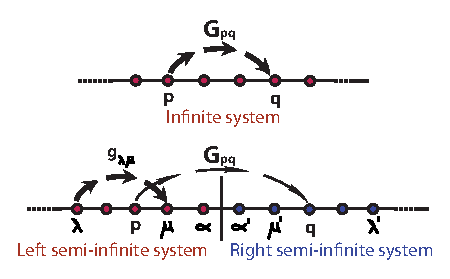
\includegraphics{fig3.eps}
\caption{(top) Representation of an infinite chain. $\h G_{pq}$ is the infinite Green's function that propagates the electron from site $p$ to site $q$. (bottom) Representation of two semi-infinite chains. $\h g_{\lam \mu}$ is the left semi-infinite Green's function that propagates the electron from site $j=\lam$ to site $j=\mu$.}
\label{dyson}
\end{figure}
%%%%%%%%%%%


In particular from Eq. \eqref{dysonseminf} we have, $\h G_{q\alp}= \h g_{q\alp'} t_{\alp'\alp} \h G_{\alp \alp}$ and  $\h G_{p\alp'}= \h g_{p\alp} t_{\alp\alp'} \h G_{\alp' \alp'}$, where $\h g_{ q\alp} = 0$ and $\h g_{p\alp'}=0$ as each pair of subindexes correspond to different semi-infinite regions. Rearranging we have,

\begin{align}
\label{202}
\h g^\sg_{q\alp'} = \frac{\h G^\sg_{q\alp}}{ t_{\alp'\alp} \h G^\sg_{\alp \alp}} =   \frac{ n^{\sg^{|q-\alp|}}}{ t_{\alp'\alp}  }, \\
\h g^\sg_{p\alp}  = \frac{\h G^\sg_{p\alp'}}{t_{\alp\alp'} \h G^\sg_{\alp' \alp'}} =  \frac{ n^{\sg^{|p-\alp'|}}}{ t_{\alp\alp'}  },
\label{203}
\end{align}

where $\sg$ is either $\upa$ or $\dna$. Considering  $n^{\sg} = (\chi^{\sg } - i\sqrt{1 -\chi^{2 \sg }  }) $ then

\begin{align}
n^{\sg^{-1}}  = \frac{1}{n^{\sg}} = \frac{1}{(\chi^{\sg } - i\sqrt{1 -\chi^{2 \sg }  })}\frac{(\chi^{\sg } + i\sqrt{1 -\chi^{2 \sg }  })}{(\chi^{\sg } + i\sqrt{1 -\chi^{2 \sg }  })} = (\chi^{\sg } + i\sqrt{1 -\chi^{2 \sg }  }) = n^{*\sg}. 
\end{align}

Consequently 

\begin{align}
-i(n^{\sg^{-1}} - n^{\sg}) = 2\sqrt{1 -\chi^{2 \sg } }.
\label{topn}
\end{align}

Since $d^{\sg} = \sqrt{ 4t^2 - (E-\eps_{\bm k_\para} - \eps_\Og^{\sg})^2 } $ and $\chi^{\sg} = \frac{E-\eps_{\bm{k}_{||}}- \eps_\Og^{\sg}}{2t}$ then $d^{\sg}  = 2t \sqrt{1-\chi^{2 \sg }}$. Therefore, Eq. \eqref{topn} becomes,

\begin{align}
\frac{1}{t} = -i\frac{(n^{\sg^{-1}} - n^{\sg})}{d^\sg}.
\label{topn2}
\end{align}

Making use of Eq. \eqref{topn2} we re-express Eqs. \eqref{202}-\eqref{203} as,

\begin{align}
\label{2022}
\h g^\sg_{q\alp'} =  -i\frac{n^{\sg^{|q-\alp|}}(n^{\sg^{-1}} - n^{\sg})}{d^\sg} , \\
\h g^\sg_{p\alp}  =  -i\frac{n^{\sg^{|p-\alp'|}}(n^{\sg^{-1}} - n^{\sg})}{d^\sg}.
\label{2033}
\end{align}

As seen in Fig. \ref{dyson}, to consider subindexes of the same semi-infinite region we take $\alp' = \alp + 1$, where $q>\alp'$ and $p<\alp$ then,

\begin{align}
\label{20222}
\h g^\sg_{q\alp'} =  -i\frac{n^{\sg^{(q-(\alp'-1))}}(n^{\sg^{-1}} - n^{\sg})}{d^\sg} = -i\frac{(n^{\sg^{(q-\alp')}} - n^{\sg^{(q-\alp'+2)}})}{d^\sg} , \\
\h g^\sg_{p\alp}  =  -i\frac{n^{\sg^{-(p-(\alp+1))}}(n^{\sg^{-1}} - n^{\sg})}{d^\sg} =  -i\frac{(n^{\sg^{-p+\alp}} - n^{\sg^{-p+\alp+2}})}{d^\sg} .
\label{20333}
\end{align}

From now on it is enough to consider the positive semi-infinite region. we choose $\alp'=1$ then,
\begin{align}
\label{202222}
\h g^\sg_{q1} =   -i\frac{(n^{\sg^{(q-1)}} - n^{\sg^{(q+1)}})}{d^\sg}. \\
\end{align}

For the rest of the matrix elements with $l,m \geq \alp'$ we apply Dyson's equation,

\begin{align}
\h G_{lm} = \h g_{lm} + \h g_{l\alp'}t\h G_{\alp m} \rightarrow \h g_{lm} = \h G_{lm} -  \h g_{l\alp'}t\h G_{\alp m}
\end{align}

Using Eq. \eqref{202222} it becomes,

\begin{align}
\h g^\sg_{lm} &= \h G^\sg_{lm} -  \h g^\sg_{l\alp'}t\h G^\sg_{\alp m} \nn\\
&= -i \frac{n^{\sg^{|l-m|}}}{d^\sg} - i^2\frac{(n^{\sg^{(l-1)}} - n^{\sg^{(l+1)}})}{d^\sg}t\frac{n^{\sg^m}}{d^\sg} \nn\\
&=-i \frac{n^{\sg^{|l-m|}}}{d^\sg} + \frac{(n^{\sg^{(l+m-1)}} - n^{\sg^{(l+m+1)}})}{d^{\sg^2}}t \nn\\
&=-i \frac{n^{\sg^{|l-m|}}}{d^\sg} + n^{\sg^{(l+m)}}\frac{(n^{\sg^{-1}} - n^{\sg^{1}})}{d^{\sg^2}}t \nn\\
&=-i \frac{n^{\sg^{|l-m|}}}{d^\sg} + i\frac{n^{\sg^{(l+m)}}}{d^\sg} \nn\\
&=-i \bigg{[} \frac{n^{\sg^{|l-m|}}}{d^\sg} - \frac{n^{\sg^{(l+m)}}}{d^\sg} \bigg{]}
\end{align}


Considering Eqs. \eqref{retseminfother}-\eqref{retseminf2other}, for an arbitrary direction of the magnetization the retarded component of the semi-infinite Green's function is expressed as,


\begin{align}
\label{xx1}
\h g^{r,\upa\upa(\dna\dna)}(l,m;E)&= -\frac{i}{2}\Bigg{[}(1\pm\cos\theta)\frac{n^{\upa|l-m|}-n^{\upa(l+m)}}{d^\upa} + (1\mp\cos\theta)\frac{n^{\dna|l-m|}-n^{\dna(l+m)}}{d^\dna}\Bigg{]}, \\
\h g^{r,\dna\upa(\upa\dna)}(l,m;E)&= -\frac{i}{2}\Bigg{[}\sin\theta e^{\pm i\phi}\frac{n^{\upa|l-m|}}{d^\upa} - \sin\theta e^{\pm i\phi}\frac{n^{\dna |l-m|}}{d^\dna}+\sin\theta e^{\pm i\phi}\frac{n^{\dna(l+m)}}{d^\dna}-\sin\theta e^{\pm i\phi}\frac{n^{\upa(l+m)}}{d^\upa}\Bigg{]}.
\label{xx2}
\end{align}


%%%%%%%%%%%%%%
\subsection{Coupled Green's functions}
For a finite system in contact with two electrodes, the Hamiltonian given in Eq. \eqref{eq:hamiltonian} in its block form reads,

\begin{align}
\bm{\h H} = \left(\begin{matrix}
\h H_{left} & \h H_{left-finite} & 0 \\
\h H^\dagger_{left-finite} & \hat H_{finite} & \h H_{right-finite}^\dagger \\
0 & \h H_{right-finite} & \h H_{right} 
\end{matrix} \right),
\label{blockh}
\end{align}

where $\h H_{left-finite}$ and $\h H_{right-finite}$ are the two components of the interaction Hamiltonian given in Eq. \eqref{eq:int}. For simplicity we consider here the case where the finite region is given entirely by the barrier, i.e., $\h H_{finite}=\h H_B$ and $\h H_{left (right)} = \h H_{L(R)}$. Schrodinger's equation in the Green's function representation is given by,

\begin{align}
\left(\begin{matrix}
E- \h H_L & -\h H_{LF} & 0 \\
-\h H^\dagger_{LF} & E- \hat H_F & -\h H_{RF}^\dagger \\
0 & -\h H_{RF} & E- \h H_{R} 
\end{matrix} \right) 
\left(\begin{matrix}
\h G_{LL} & \h G_{LF} & 0 \\
\h G_{FL} & \hat G_{FF} & \h G_{FR} \\
0 & \h G_{RF} & \h G_{RR} 
\end{matrix} \right) 
= \h I,
\label{blockgf}
\end{align}

which gives rise to a solution of the form $(E-\h H_{F} - \h \Sg)\h G_{FF}= \h I$, with $\h \Sg = \h H_{LF}^\dg(E-\h H_L)^{-1} \h H_{LF} + \h H_{RF}^\dg (E-\h H_R)^{-1} \h H_{RF}$. Replacing Eq. \eqref{eq:int} in the definition of $\h \Sg$ we have, $\h \Sg = t_{a\alp} \h g_{\alp\alp} t_{\alp a} + t_{b\alp'} \h g_{\alp'\alp'}t_{\alp' b}$, where site $\alp$ ($\alp'$) in the left (right) electrode is next to site  $a$ ($b$) in the finite region, see left panel in Fig. \ref{junction}. Notice that $\h g_{\alp\alp(\alp'\alp')}$ is the $2\times2$ isolated semi-infinite retarded Green's function matrix derived in the previous section. In what follows, upper-index $r$ is removed for simplicity. $\h \Sg$ describes the propagation of the electron across the interfaces and is referred to as the self energy term. It can be partitioned in two components,

\begin{align}
\label{selfleft}
{\hat \Sg}_{aa}=t_{a\alp}\h g_{\alp\alp}t_{\alp a}, ~~~~~~~~~~~~~~{\hat \Sg}_{bb}=t_{b\alp'} \h g_{\alp'\alp'}t_{\alp'b}.
\end{align}

We now proceed to couple the full system made of semi-infinite electrodes and a finite system. For this we solve a system of Dyson's equations of the form

\begin{align}
{\hat G}_{pq}={\hat g}_{pq}+{\hat g}_{pa}{\hat \Sg}_{aa}{\hat G}_{aq}+{\hat g}_{pb}{\hat \Sg}_{bb}{\hat G}_{bq},
\label{eq:dyson}
\end{align}

where $\h G$ ($\h g$) is the $2\times2$ coupled (isolated) retarded Green's function matrix. $p$ and $q$ denote  atomic sites in the finite region.  Eq. \eqref{eq:dyson} is self-consistent, which means that each coupled Green's function can be described in terms of isolated Green's functions. For example we have,

\begin{align}
\label{eq:dysona}
{\hat G}_{aq}&= (I-\h g_{aa}\h \Sg_{aa})^{-1}\h g_{aq} + (I-\h g_{aa}\h \Sg_{aa})^{-1}\h g_{ab}\h \Sg_{bb}\h G_{bq}, \\
{\hat G}_{bq}&= (I-\h g_{bb}\h \Sg_{bb})^{-1}\h g_{bq} + (I-\h g_{bb}\h \Sg_{bb})^{-1}\h g_{ba}\h \Sg_{aa}\h G_{aq}.
\label{eq:dysonb}
\end{align}

Replacing Eq. \eqref{eq:dysonb} in Eq. \eqref{eq:dysona}, we get,

 \begin{align}
\label{eq:dysonab}
{\hat G}_{aq}&= (I-(I-\h g_{aa}\h \Sg_{aa})^{-1}\h g_{ab}\h \Sg_{bb}(I-\h g_{bb}\h \Sg_{bb})^{-1}\h g_{ba}\h \Sg_{aa})^{-1}(I-\h g_{aa}\h \Sg_{aa})^{-1}\h g_{aq} \nn\\
&+ (I-(I-\h g_{aa}\h \Sg_{aa})^{-1}\h g_{ab}\h \Sg_{bb}(I-\h g_{bb}\h \Sg_{bb})^{-1}\h g_{ba}\h \Sg_{aa})^{-1}(I-\h g_{aa}\h \Sg_{aa})^{-1} \h g_{ab}\h \Sg_{bb}(I-\h g_{bb}\h \Sg_{bb})^{-1}\h g_{bq}.
\end{align}

Similarly replacing Eq. \eqref{eq:dysona} in Eq. \eqref{eq:dysonb},

 \begin{align}
\label{eq:dysonab}
{\hat G}_{bq}&= (I-(I-\h g_{bb}\h \Sg_{bb})^{-1}\h g_{ba}\h \Sg_{aa}(I-\h g_{aa}\h \Sg_{aa})^{-1}\h g_{ab}\h \Sg_{bb})^{-1}(I-\h g_{bb}\h \Sg_{bb})^{-1}\h g_{bq} \nn\\
&+ (I-(I-\h g_{bb}\h \Sg_{bb})^{-1}\h g_{ba}\h \Sg_{aa}(I-\h g_{aa}\h \Sg_{aa})^{-1}\h g_{ab}\h \Sg_{bb})^{-1}(I-\h g_{bb}\h \Sg_{bb})^{-1} \h g_{ba}\h \Sg_{aa}(I-\h g_{aa}\h \Sg_{aa})^{-1}\h g_{aq}.
\end{align}

Considering,

\begin{align}
\h \Sg_L &= \h \Sg_{aa}= t_{a\alp}\h g_{\alp\alp}t_{\alp a}, \\
\h \Sg_R &= \h \Sg_{bb}= t_{b\alp'}\h g_{\alp' \alp'} t_{\alp' b},
\end{align}

 \begin{align}
 \tx{invA} &= (I - \h g_{aa}\h \Sg_L)^{-1}, \\
 \tx{invB} &= (I - \h g_{bb}\h \Sg_R)^{-1},
 \end{align}
 
 \begin{align}
 \tx{invDen1} = (I-(I-\h g_{aa}\h \Sg_{aa})^{-1}\h g_{ab}\h \Sg_{bb}(I-\h g_{bb}\h \Sg_{bb})^{-1}\h g_{ba}\h \Sg_{aa})^{-1}, \\
 \tx{invDen2} =  (I-(I-\h g_{bb}\h \Sg_{bb})^{-1}\h g_{ba}\h \Sg_{aa}(I-\h g_{aa}\h \Sg_{aa})^{-1}\h g_{ab}\h \Sg_{bb})^{-1}.
 \end{align}

Then,

 \begin{align}
\label{eq:nino}
{\hat G}_{aq}&= (\tx{invDen1})(\tx{invA})(\h g_{aq} + \h g_{ab} \h \Sg_R \tx{invB}\h g_{bq}), \\
{\hat G}_{bq}&= (\tx{invDen2})(\tx{invB})(\h g_{bq} + \h g_{ba} \h \Sg_L \tx{invA}\h g_{aq}), \\
{\hat G}_{pq}& ={\hat g}_{pq}+{\hat g}_{pa}{\hat \Sg}_{L}{\hat G}_{aq}+{\hat g}_{pb}{\hat \Sg}_{R}{\hat G}_{bq}.
\label{eq:nino2}
\end{align}

Similar calculations are performed for the advanced Green's functions,  ${\hat {G}}^a_{pq}$, given as the Hermitian conjugate of $\h G_{pq}$.


%%%%%%%%%%%%%%%
%%%%%%%%%%%%
\subsection{Lesser Green's functions: Quantum Kinetic Equation}

In its matrix form, Dyson's equation in Keldysh formalism reads, \cite{keldysh}
\begin{equation}
\left[ {\begin{array}{cc}
0 & \h{G}^a_{pq} \\
\h G^r_{pq} & \h F_{pq}
\end{array}} \right] = \left[ {\begin{array}{cc}
0 & \h{g}^a_{pq} \\
\h g^r_{pq} & \h f_{pq}
\end{array}} \right] + 
\left[ {\begin{array}{cc}
0 & \h{g}^a_{pq_1}\h {\Sg}^a_{q_1,q_2} \h{G}^a_{q_2 q} \\
\h{g}^r_{pq_1}\h {\Sg}^r_{q_1,q_2} \h{G}^r_{q_2 q}     &  g^r_{p,q_1} \h \Og_{q_1,q_2} \h G^a_{q_2 q}  + g^r_{p,q_1} \h \Sg^r_{q_1,q_2} \h F_{q_2 q} + \h f_{pq_1} \h \Sg^a_{q_1q_2} \h{G}^a_{q_2 q}
\end{array}} \right],
\end{equation}

which leads to three equations of the form,

\begin{align}
\label{big1}
\h{G}^a_{pq} &= \h{g}^a_{pq}  + \h{g}^a_{pq_1}\h {\Sg}^a_{q_1,q_2} \h{G}^a_{q_2 q} \\
\label{big2}
\h G^r_{pq} &= \h g^r_{pq} + \h{g}^r_{pq_1}\h {\Sg}^r_{q_1,q_2} \h{G}^r_{q_2 q} \\
 \h F_{pq} &= \h f_{pq} + g^r_{p,q_1} \h \Og_{q_1,q_2} \h G^a_{q_2 q}  + g^r_{p,q_1} \h \Sg^r_{q_1,q_2} \h F_{q_2 q} + \h f_{pq_1} \h \Sg^a_{q_1q_2} \h{G}^a_{q_2 q}
\label{big3}
\end{align}

The first two are the usual Dyson's equations for the advanced ($\h G^a)$ and retarded ($\h G^r$) Green's functions. The third one is referred to as the non-equlibrium Dyson's equation for the Keldysh function ($\h F$). Considering the leads to give an instantaneous perturbation,\cite{caroli} the self-energy reads,

\begin{align}
\label{qkeself2}
\h \Sg_{q_1q_2} = t (\dlt_{q_1\alp} \dlt_{aq_2} + \dlt_{q_1 a}\dlt_{\alp q_2}) + t' (\dlt_{q_1 b}\dlt_{\alp'q_2} + \dlt_{q_1\alp'}\dlt_{b q_2}),
\end{align}

with $\h \Og = 0$, $\h \Sg^r=\h \Sg^a = \h \Sg$.
In Keldysh formalism the following relationships hold among the Green's functions,

\begin{align}
\label{menor1}
\h G^<_{pq} &= \frac{1}{2 }[\h F_{pq} + \h G^a_{pq} - \h G^r_{pq}], \\
\h g^<_{pq} &= \frac{1}{2 }[\h f_{pq} + \h g^a_{pq} - \h g^r_{pq}]. 
\label{menor2}
\end{align}

Replacing Eqs. \eqref{menor1}-\eqref{menor2} in Eq. \eqref{big3} we have,

\begin{align}
2\h G^<_{pq} -\h G^a_{pq}+\h G^r_{pq} &= 2\h g^<_{pq} -  \h g^a_{pq}  +\h g^r_{pq}  + g^r_{p,q_1} \h \Sg_{q_1,q_2} (2\h G^<_{q_2 q}- \h G^a_{q_2 q}+\h G^r_{q_2 q}) + (2\h g^<_{pq_1} - \h g^a_{pq_1} + \h g^r_{pq_1}  ) \h \Sg_{q_1q_2} \h{G}^a_{q_2 q}, \nn\\
&=2\h g^<_{pq} -  \h g^a_{pq}  +\h g^r_{pq}  + g^r_{p,q_1} \h \Sg_{q_1,q_2} (2\h G^<_{q_2 q}+\h G^r_{q_2 q}) + (2\h g^<_{pq_1} - \h g^a_{pq_1}   ) \h \Sg_{q_1q_2} \h{G}^a_{q_2 q}, \nn\\
&=2\h g^<_{pq} + 2 g^r_{p,q_1} \h \Sg_{q_1,q_2} \h G^<_{q_2 q} + 2\h g^<_{pq_1}\h \Sg_{q_1q_2} \h{G}^a_{q_2 q} -  \h g^a_{pq}  +\h g^r_{pq}  + g^r_{p,q_1} \h \Sg_{q_1,q_2} \h G^r_{q_2 q} - \h g^a_{pq_1}  \h \Sg_{q_1q_2} \h{G}^a_{q_2 q}. 
\label{menor3}
\end{align}

Notice in Eq. \eqref{menor3} that Eqs. \eqref{big1}-\eqref{big2} appear; therefore,

\begin{align}
\h G^<_{pq}=\h g^<_{pq} +  g^r_{p,q_1} \h \Sg_{q_1,q_2} \h G^<_{q_2 q} + \h g^<_{pq_1}\h \Sg_{q_1q_2} \h{G}^a_{q_2 q}, 
\label{menor3o}
\end{align}

which corresponds to the non-equilibrium Dyson's equation for the Lesser Green's function. Considering Eq. \eqref{qkeself2} we see that the self-energy is non-zero only in four particular cases: ($q_1=\alp,  q_2= a$), ($q_1=a,  q_2= \alp$), ($q_1=b,  q_2= \alp'$), and  ($q_1=\alp',  q_2= b$). Consequently the full expression reads,
 
 \begin{align}
 \label{fullself5}
 \h G^<_{pq} = \h g^<_{pq} &+ t(\h g^r_{p\alp}\h G^<_{aq} + \h g^r_{pa} \h G^<_{\alp q} +  \h g^<_{p\alp} \h{G}^a_{aq} + \h g^<_{pa}\h{G}^a_{\alp q})
  +t' (\h g^r_{pb}\h G^<_{\alp' q} + \h g^r_{p\alp'}\h G^<_{bq} +  \h g^<_{pb} \h{G}^a_{\alp' q} + \h g^<_{p\alp'}\h{G}^a_{bq}). 
 \end{align}
 
 To derive the Lesser Green's function $(\h G_{ij}^<$) in the finite region ($i,j$ $\eps$ finite system) we take into account that $g^<$ and $g$ are defined as isolated contributions; therefore, they vanish when $i$ and $j$ points are taken in different subparts of the junctions, e.g., $g^r_{\alp,j}=0$. Therefore, the above expression simplifies to,
 
  \begin{align}
 \label{fullself5o}
 \h G^<_{ij} = \h g^<_{iq} & + t \h g^r_{ia} \h G^<_{\alp j}  +t \h g^<_{ia}\h{G}^a_{\alp j} +t' \h g^r_{ib}\h G^<_{\alp' j}  + t' \h g^<_{ib} \h{G}^a_{\alp' j} . 
 \end{align}

In the original Caroli's paper,\cite{caroli} the finite region was treated as a barrier to get rid of initial electron occupation given by $g^<$, i.e., the density of states becomes zero due to tunneling effect; being it related to the imaginary part of the Green's functions, then the latter become real, $g^a = g^r = g_{ij}$ and $g^<_{ij}=0$. In a more general approach, the finite region may consider metallic states; nonetheless, after tedious calculations (not presented here) it is shown that even in the presence of metallic states we have $g^<_{ij}=0$ in the finite region. From a physical point of view it means that when the system reaches the steady state, its non-equilibrium occupation will be solely determined by the chemical potentials of the leads and the system will "forget" its initial occupation. Of course, this approach is valid only for the steady state limit. Mathematically it implies that the above expression reduces to,

 
  \begin{align}
  \label{Fij5}
 \h G^<_{ij} =   t \h g^r_{ia} \h G^<_{\alp j}  +t' \h g^r_{ib}\h G^<_{\alp' j}. 
   \end{align}
 
Considering Eq. \eqref{fullself5} we also have,

  \begin{align}
  \label{ni15}
 \h G^<_{\alp j} &=   t \h g^<_{\alp\alp} \h{G}^a_{a j}  +t \h g^r_{\alp\alp}\h G^<_{a j}, \\
    \label{ni25}
   \h G^<_{\alp' j} &=   t' \h g^r_{\alp'\alp'} \h{G}^<_{b j}  +t' \h g^<_{\alp'\alp'}\h{G}^a_{b j}, \\
    \label{ni35}
    \h G^<_{a j} &=   t \h g^r_{a a} \h{G}^<_{\alp j}  +t' \h g^r_{a b}\h G^<_{\alp' j}, \\
      \label{ni45}
      \h G^<_{b j} &=   t \h g^r_{b a} \h{G}^<_{\alp j}  +t' \h g^r_{b b}\h G^<_{\alp' j}. 
   \end{align}
 
Replacing Eq. \eqref{ni35} in \eqref{ni15} we have,

\begin{align}
\label{ni55}
\h G^<_{\alp j} &=   t \h g^<_{\alp\alp} \h{G}^a_{a j}  +t \h g^r_{\alp\alp}(t \h g^r_{a a} \h{G}^<_{\alp j}  +t' \h g^r_{a b}\h G^<_{\alp' j}) \nn\\
&= t \h g^<_{\alp\alp} \h{G}^a_{a j}  + \h \Sg_{L} \h g^r_{a a} \h{G}^<_{\alp j}  +\h \Sg_{L} g^r_{a b}\h G^<_{\alp' j}, \nn\\
\h G^<_{\alp j} &= (I-\h \Sg_L \h g^r_{aa})^{-1} t g^<_{\alp\alp} \h{G}^a_{aj} + (I-\h \Sg_L \h g^r_{aa})^{-1} \h \Sg_L \h g^r_{ab} \h G^<_{\alp' j}.
\end{align}

Replacing Eq.  \eqref{ni45} in \eqref{ni25} we have,

\begin{align}
\label{ni65}
\h G^<_{\alp' j} &=   t' \h g^r_{\alp'\alp'} ( t \h g^r_{b a} \h{G}^<_{\alp j}  +t' \h g^r_{b b}\h G^<_{\alp' j} ) +t' \h g^<_{\alp'\alp'}\h{G}^a_{b j} \nn\\
&= \h \Sg_R  \h g^r_{b a} \h{G}^<_{\alp j} + \h \Sg_R  \h g^r_{b b}\h G^<_{\alp' j}+t' \h g^<_{\alp'\alp'}\h{G}^a_{b j}, \nn\\
\h G^<_{\alp' j} &= (I- \h \Sg_R  \h g^r_{b b})^{-1}\h \Sg_R  \h g^r_{b a} \h{G}^<_{\alp j} + (I- \h \Sg_R  \h g^r_{b b})^{-1}t' \h g^<_{\alp'\alp'}\h{G}^a_{b j}.
\end{align}


Replacing Eq. \eqref{ni65} in \eqref{ni55} we have,

\begin{align}
\label{ni75}
\h G^<_{\alp j} &= [I - (I-\h \Sg_L \h g^r_{aa})^{-1} \h \Sg_L \h g^r_{ab}(I- \h \Sg_R  \h g^r_{b b})^{-1}\h \Sg_R  \h g^r_{b a}]^{-1}(I-\h \Sg_L \h g^r_{aa})^{-1} t g^<_{\alp\alp} \h{G}^a_{aj} \nn\\&+ [I - (I-\h \Sg_L \h g^r_{aa})^{-1} \h \Sg_L \h g^r_{ab}(I- \h \Sg_R  \h g^r_{b b})^{-1}\h \Sg_R  \h g^r_{b a}]^{-1}(I-\h \Sg_L \h g^r_{aa})^{-1} \h \Sg_L \h g^r_{ab} (I- \h \Sg_R  \h g^r_{b b})^{-1}t' \h g^<_{\alp'\alp'}\h{G}^a_{b j}.
\end{align}

Replacing Eq. \eqref{ni55} in \eqref{ni65} we have,

\begin{align}
\label{ni85}
\h G^<_{\alp' j} &= [I - (I- \h \Sg_R  \h g^r_{b b})^{-1}\h \Sg_R  \h g^r_{b a}(I-\h \Sg_L \h g^r_{aa})^{-1} \h \Sg_L \h g^r_{ab} ]^{-1}(I- \h \Sg_R  \h g^r_{b b})^{-1}\h \Sg_R  \h g^r_{b a}(I-\h \Sg_L \h g^r_{aa})^{-1} t g^<_{\alp\alp} \h{G}^a_{aj} \nn\\& + [I - (I- \h \Sg_R  \h g^r_{b b})^{-1}\h \Sg_R  \h g^r_{b a}(I-\h \Sg_L \h g^r_{aa})^{-1} \h \Sg_L \h g^r_{ab} ]^{-1}(I- \h \Sg_R  \h g^r_{b b})^{-1}t' \h g^<_{\alp'\alp'}\h{G}^a_{b j}.
\end{align}

Considering

\begin{align}
\label{def15}
\tx{invDen1}&= [I - (I-\h \Sg_L \h g^r_{aa})^{-1} \h \Sg_L \h g^r_{ab}(I- \h \Sg_R  \h g^r_{b b})^{-1}\h \Sg_R  \h g^r_{b a}]^{-1}, \\
\tx{invDen2}&= [I - (I- \h \Sg_R  \h g^r_{b b})^{-1}\h \Sg_R  \h g^r_{b a}(I-\h \Sg_L \h g^r_{aa})^{-1} \h \Sg_L \h g^r_{ab} ]^{-1}, \\
\tx{invA}&=(I-\h \Sg_L \h g^r_{aa})^{-1}, \\
\tx{invB}&=(I- \h \Sg_R  \h g^r_{b b})^{-1},
\label{def25}
\end{align}

we have,

\begin{align}
\label{ni105}
\h G^<_{\alp j} &= (\tx{invDen1})(\tx{invA}) t g^<_{\alp\alp} \h{G}^a_{aj}+ (\tx{invDen1})(\tx{invA}) \h \Sg_L \h g^r_{ab} (\tx{invB})t' \h g^<_{\alp'\alp'}\h{G}^a_{b j}, \\
\h G^<_{\alp' j} &= (\tx{invDen2})(\tx{invB})\h \Sg_R  \h g^r_{b a}(\tx{invA}) t g^<_{\alp\alp} \h{G}^a_{aj} + (\tx{invDen2})(\tx{invB})t' \h g^<_{\alp'\alp'}\h{G}^a_{b j}.
\label{ni115}
\end{align}

Notice that Eqs. \eqref{def15}-\eqref{def25} are different from the ones given in the previous section. Replacing Eqs. \eqref{ni105}-\eqref{ni115} in Eq. \eqref{Fij5} we have,

  \begin{align}
  \label{Fij25}
 \h G^<_{ij} &=   t^2 \h g^r_{ia} (\tx{invDen1})(\tx{invA}) g^<_{\alp\alp} \h{G}^a_{aj} +t^2 \h g^r_{ib}(\tx{invDen2})(\tx{invB})\h \Sg_R  \h g^r_{b a}(\tx{invA})  g^<_{\alp\alp} \h{G}^a_{aj} \nn\\& 
  + t^2 \h g^r_{ib}(\tx{invDen2})(\tx{invB}) \h g^<_{\alp'\alp'}\h{G}^a_{b j}+t^2 \h g^r_{ia} (\tx{invDen1})(\tx{invA}) \h \Sg_L \h g^r_{ab} (\tx{invB}) \h g^<_{\alp'\alp'}\h{G}^a_{b j}. 
   \end{align}

Considering

\begin{align}
\h f_{\alp\alp} &= (1-2f_L)(g^r_{\alp\alp}-\h{g}^a_{\alp\alp}),\\
\h f_{\alp'\alp'} &= (1-2f_R)(g^r_{\alp'\alp'}-\h{g}^a_{\alp'\alp'}),
\end{align}

where the Fermi Dirac distribution is given by,

\begin{align}
f_L = \frac{1}{e^{\frac{E-\mu_L}{k_B T} } + 1}, \\
f_R = \frac{1}{e^{\frac{E-\mu_R}{k_B T} } + 1},
\end{align}

and the usual definition,

\begin{align}
\h g^<_{pq} = \frac{1}{2 }[\h f_{pq} + \h g^a_{pq} - \h g^r_{pq}],
\end{align}

we have,

\begin{align}
\h g^<_{\alp\alp} &= - f_L(\h g^r_{\alp\alp}-\h{g}^a_{\alp\alp}),\\
\h g^<_{\alp'\alp'} &= - f_R(\h g^r_{\alp'\alp'}-\h{g}^a_{\alp'\alp'}).
\end{align}


   
Eq. \eqref{Fij25} is our final expression for the Lesser Green's function.

%%%%%%%%%%%%%%%%%%%%%%%
%%%%%%%%%%%%%%%%%%%%%%%%%
\section{Charge Current Density}

In the following, we proceed to derive the charge current density for our tunnel junction made of semi-infinite electrodes and a finite region.

%%%%%%%%%%%%%%%%%%%%%%%%%%
\subsection{General definition in second quantization}

Let P be a point between sites i and i+1 (see Fig. 1), the current at point P is the difference between the flow of electrons from left to right and from right to left. We thus expect an operator of the form,

\begin{align}
J_P = \sum_{l \geq i+1, m \leq i} A_{ml} c^\dagger_l c_m - \sum_{l \leq i, m \geq i+1} A_{ml}c^\dagger_l c_m,
\label{jp}
\end{align}

And if we take the current at point P', we have

\begin{align}
J_{P'}= \sum_{l \geq i, m \leq i-1} A_{ml} c^\dagger_l c_m - \sum_{l \leq i-1, m \geq i} A_{ml}c^\dagger_l c_m,
\label{jpp}
\end{align}

where the first term refers to the flow from left to right and the second term from right to left. Notice that we are neglecting the spin for simplicity.

%%%%%%%%%
\begin{figure}[ht]
\centering
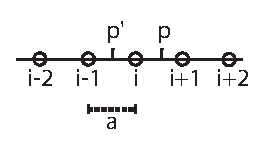
\includegraphics{fig4.eps}
\caption{Discretization of a 1D system}
\label{2ndq}
\end{figure}
%%%%%%%%%%%

To calculate $A_{lm}$ we consider the continuity equation, $-\nabla j_e = \frac{\pat \rho}{\pat t}$. In its discrete representation reads,

\begin{align}
 \frac{\pat \rho_i}{\pat t} + \frac{j_P - j_{P'}}{a} = 0.
 \label{conti}
\end{align}

$P'$ is a point between sites (i-1) and i, while $\rho_i=ec_i^\dagger c_i$ is the electron charge at site i. In Eq. \eqref{eq1} we defined any operator; therefore the Hamiltonian (H) is given in a similar form. Considering the relation $\frac{\pat \rho_i}{\pat t} = \frac{1}{i\hbar}[\rho_i, H]$ we have,

\begin{align}
\frac{\pat \rho_i}{\pat t} &= \frac{1}{i\hbar}[e c_i^\dg c_i , \sum_{lm}T_{lm}c_m^\dg c_{l}] \nn\\
&= \frac{e}{i\hbar}[c_i^\dg c_i\sum_{lm}T_{lm}c_m^\dg c_{l} - \sum_{lm}T_{lm}c_m^\dg c_{l}c_i^\dg c_i ] \nn\\
&= \frac{e}{i\hbar}[\sum_{l}T_{li}c_i^\dg c_{l} - \sum_{m}T_{im}c_m^\dg c_{i}] \nn\\
&= \frac{e}{i\hbar}\sum_{m}[T_{mi}c_i^\dg c_{m} -T_{im}c_m^\dg c_{i}]
\end{align}

For simplicity let's consider the nearest neighbor interaction, consequently summing over $m$ we have,

\begin{align}
\frac{\pat \rho_i}{\pat t} &= \frac{e}{i\hbar}[T_{i-1,i} c_i^\dg c_{i-1} + T_{i,i} c_i^\dg c_{i}+T_{i+1,i} c_i^\dg c_{i+1}-T_{i,i} c_i^\dg c_{i}-T_{i,i+1} c_{i+1}^\dg c_{i}-T_{i,i-1} c_{i-1}^\dg c_{i}] \nn\\&= \frac{e}{i\hbar}[T_{i-1,i} c_i^\dg c_{i-1} +T_{i+1,i} c_i^\dg c_{i+1}-T_{i,i+1} c_{i+1}^\dg c_{i}-T_{i,i-1} c_{i-1}^\dg c_{i}] \nn\\
&= \frac{e}{i\hbar}[T_{i-1,i} c_i^\dg c_{i-1} +T_{i+1,i} c_i^\dg c_{i+1}-h.c.]
\end{align}

Expanding Eqs. \eqref{jp}-\eqref{jpp} in the nearest neighbor approximation, we have,

\begin{align}
J_P &= \sum_{m \leq i} (A_{m,i+1} c^\dagger_{i+1} c_m+A_{m,i+2} c^\dagger_{i+2} c_m+ ... )- \sum_{m \geq i+1}( A_{m,i}c^\dagger_{i} c_m+A_{m,i-1}c^\dagger_{i-1} c_m+A_{m,i-2}c^\dagger_{i-2} c_m + ....) \nn\\
&=(A_{i,i+1} c^\dagger_{i+1} c_i )- ( A_{i+1,i}c^\dagger_{i} c_{i+1}),
\end{align}

and

\begin{align}
J_{P'}&= \sum_{m \leq i-1} (A_{mi} c^\dagger_i c_m+A_{m,i+1} c^\dagger_{i+1} c_m+A_{mi+2} c^\dagger_{i+2} c_m + ...) - \sum_{m \geq i}(A_{m,i-1}c^\dagger_{i-1} c_m+A_{m,i-2}c^\dagger_{i-2} c_m + ...) \nn\\
&= (A_{i-1,i} c^\dagger_i c_{i-1}) -(A_{i,i-1}c^\dagger_{i-1} c_i)
\end{align}

Making use of the continuity equation (Eq. \eqref{conti}) we have,


\begin{align}
\frac{ea}{i\hbar}[T_{i-1,i} c_i^\dg c_{i-1} +T_{i+1,i} c_i^\dg c_{i+1}-h.c.]&= [(A_{i-1,i} c^\dagger_i c_{i-1}) -(A_{i,i-1}c^\dagger_{i-1} c_i)]-[(A_{i,i+1} c^\dagger_{i+1} c_i )- ( A_{i+1,i}c^\dagger_{i} c_{i+1})]  \nn\\
& = (A_{i-1,i} c^\dagger_i c_{i-1}) + ( A_{i+1,i}c^\dagger_{i} c_{i+1}) - h.c.
\end{align}

Therefore, $\frac{ea}{i\hbar} T_{ml} = A_{ml}$ and the charge current becomes


\begin{align}
J_P &= \frac{ea}{i\hbar} \sum_{\sg,\sg'}[T^{\sg,\sg'}_{i,i+1} c^{\dagger\sg'}_{i+1} c^{\sg}_i - h.c.] \nn\\
&=\frac{ea}{i\hbar} [T^{\upa,\upa}_{i,i+1} c^{\dagger\upa}_{i+1} c^{\upa}_i+T^{\dna,\upa}_{i,i+1} c^{\dagger\upa}_{i+1} c^{\dna}_i + T^{\upa,\dna}_{i,i+1} c^{\dagger\dna}_{i+1} c^{\upa}_i+T^{\dna,\dna}_{i,i+1} c^{\dagger\dna}_{i+1} c^{\dna}_i   - h.c.],
\label{corriente}
\end{align}

where we have inserted the spin contribution.


%%%%%%%%%%%%%%%%%%%
\subsection{Charge current density in the presence of Rashba along the $xz$-plane}

%%%%%%%%%%%%%%%%%%
\subsubsection{Anomalous current}
In the previous section we considered the Hamiltonian in its general form,

\begin{align}
\label{eqminus1}
\hat{H} &= \sum_{i,j,\sigma,\sigma'} T_{i,j}^{\sigma,\sigma'} \hat{c}_j^{\dagger \sigma'} \hat{c}^\sigma_i, \\
&=  \sum_{i,j} T_{i,j}^{\uparrow,\uparrow} c_j^{\dagger \uparrow} c_i^\uparrow + T_{i,j}^{\uparrow,\downarrow} c_j^{\dagger \downarrow} c_i^\uparrow + T_{i,j}^{\downarrow,\uparrow} c_j^{\dagger \uparrow} c_i^\downarrow + T_{i,j}^{\downarrow,\downarrow} c_j^{\dagger \downarrow} c_i^\downarrow
\end{align}

and out of it we retrieved a definition of the charge current around point P as,

\begin{align}
J_P &=\frac{ea}{i\hbar} [T^{\upa,\upa}_{i,i+1} c^{\dagger\upa}_{i+1} c^{\upa}_i+T^{\dna,\upa}_{i,i+1} c^{\dagger\upa}_{i+1} c^{\dna}_i + T^{\upa,\dna}_{i,i+1} c^{\dagger\dna}_{i+1} c^{\upa}_i+T^{\dna,\dna}_{i,i+1} c^{\dagger\dna}_{i+1} c^{\dna}_i   - h.c.].
\label{corriente222}
\end{align}


Notice that this expression is general and subindex $i$ may refer to any direction in a three dimensional system. The Hamiltonian given in Eq. \eqref{eqminus1} can be separated in two components, the usual free-electron component and the anomalous component,

\begin{align}
\h H = \h H_0 + \h H_{so}
\end{align}
In \S  \ref{sec:rashbamatrix} the anomalous component was redefined as $\h H_{so} = \h H_{so}^X + \h H_{so}^Z$, where  

\begin{align}
\label{hsoxxxo}
\hat H^X_{so} &= \sum_{i} \frac{\lambda_{so}^*}{2a}  \Bigg{\{} c_{i+1}^{\dagger \uparrow} c_{i}^\uparrow - c_{i}^{\dagger \uparrow} c_{i+1}^\uparrow  - c_{i+1}^{\dagger \downarrow} c_{i}^\downarrow + c_{i}^{\dagger \downarrow} c_{i+1}^\downarrow \Bigg{\}}, \nn\\
&=\frac{\lambda_{so}^*}{2a}  \Bigg{\{} c_{i+1}^{\dagger \uparrow} c_{i}^\uparrow  + c_{i}^{\dagger \uparrow} c_{i-1}^\uparrow - c_{i}^{\dagger \uparrow} c_{i+1}^\uparrow  - c_{i-1}^{\dagger \uparrow} c_{i}^\uparrow - c_{i+1}^{\dagger \downarrow} c_{i}^\downarrow - c_{i}^{\dagger \downarrow} c_{i-1}^\downarrow+ c_{i}^{\dagger \downarrow} c_{i+1}^\downarrow + c_{i-1}^{\dagger \downarrow} c_{i}^\downarrow + ...\Bigg{\}} \\
\hat H^Z_{so} &= \sum_{k}  \frac{\lambda_{so}^*}{2a} \Bigg{\{} -c_{k+1}^{\dagger \downarrow} c_{k}^\uparrow + c_{k}^{\dagger \downarrow} c_{k+1}^\uparrow   - c_{k+1}^{\dagger \uparrow} c_{k}^\downarrow +  c_{k}^{\dagger \uparrow} c_{k+1}^\downarrow \Bigg{\}}.
\label{hsozzzo}
\end{align}

Consequently, we can define the anomalous charge currents along $x$ and $z$ considering $\h H_{so}^X$ and $\h H_{so}^Z$ separately. It follows as general definitions,

\begin{align}
\label{eqminus1sox}
\hat{H_{so}^X} &=  \sum_{i,j} T_{i,j}^{\uparrow,\uparrow} c_j^{\dagger \uparrow} c_i^\uparrow + T_{i,j}^{\uparrow,\downarrow} c_j^{\dagger \downarrow} c_i^\uparrow + T_{i,j}^{\downarrow,\uparrow} c_j^{\dagger \uparrow} c_i^\downarrow + T_{i,j}^{\downarrow,\downarrow} c_j^{\dagger \downarrow} c_i^\downarrow, \\
\hat{H_{so}^Z} &=  \sum_{m,n} T_{m,n}^{\uparrow,\uparrow} c_n^{\dagger \uparrow} c_m^\uparrow + T_{m,n}^{\uparrow,\downarrow} c_n^{\dagger \downarrow} c_m^\uparrow + T_{m,n}^{\downarrow,\uparrow} c_n^{\dagger \uparrow} c_m^\downarrow + T_{m,n}^{\downarrow,\downarrow} c_n^{\dagger \downarrow} c_m^\downarrow, 
\label{eqminus1soz}
\end{align}

where $i$ ($m$) and $j$ ($n$) are sub-indexes along the $x$ ($z$)-axis. Comparing them with Eqs. \eqref{hsoxxxo} and \eqref{hsozzzo} the above expressions simplify to, 

\begin{align}
\label{eqminus1sox2}
\hat{H_{so}^X} &=  \sum_{i,j} T_{i,j}^{\uparrow,\uparrow} c_j^{\dagger \uparrow} c_i^\uparrow  + T_{i,j}^{\downarrow,\downarrow} c_j^{\dagger \downarrow} c_i^\downarrow = \sum_{i} \frac{\lambda_{so}^*}{2a}  \Bigg{\{} c_{i+1}^{\dagger \uparrow} c_{i}^\uparrow - c_{i}^{\dagger \uparrow} c_{i+1}^\uparrow  - c_{i+1}^{\dagger \downarrow} c_{i}^\downarrow + c_{i}^{\dagger \downarrow} c_{i+1}^\downarrow \Bigg{\}} \\
\hat{H_{so}^Z} &=  \sum_{m,n}  T_{m,n}^{\uparrow,\downarrow} c_n^{\dagger \downarrow} c_m^\uparrow + T_{m,n}^{\downarrow,\uparrow} c_n^{\dagger \uparrow} c_m^\downarrow = \sum_{k}  \frac{\lambda_{so}^*}{2a} \Bigg{\{} -c_{k+1}^{\dagger \downarrow} c_{k}^\uparrow + c_{k}^{\dagger \downarrow} c_{k+1}^\uparrow   - c_{k+1}^{\dagger \uparrow} c_{k}^\downarrow +  c_{k}^{\dagger \uparrow} c_{k+1}^\downarrow \Bigg{\}},
\label{eqminus1soz2}
\end{align}

Therefore, considering the general definition of the charge current given in Eq. \eqref{corriente222}, we have for the $x$ component

\begin{align}
j_{so}^x &=\frac{ea}{i\hbar} [T^{\upa,\upa}_{i,i+1} c^{\dagger\upa}_{i+1} c^{\upa}_i+T^{\dna,\upa}_{i,i+1} c^{\dagger\upa}_{i+1} c^{\dna}_i + T^{\upa,\dna}_{i,i+1} c^{\dagger\dna}_{i+1} c^{\upa}_i+T^{\dna,\dna}_{i,i+1} c^{\dagger\dna}_{i+1} c^{\dna}_i   - h.c.] \nn\\&= \frac{ea}{i\hbar} [T^{\upa,\upa}_{i,i+1} c^{\dagger\upa}_{i+1} c^{\upa}_i+T^{\dna,\dna}_{i,i+1} c^{\dagger\dna}_{i+1} c^{\dna}_i   - T^{\upa,\upa}_{i+1,i} c^{\dagger\upa}_{i} c^{\upa}_{i+1}-T^{\dna,\dna}_{i+1,i} c^{\dagger\dna}_{i} c^{\dna}_{i+1} ] \nn\\
&= \frac{ea}{i\hbar} [\frac{\lambda_{so}^*}{2a} c^{\dagger\upa}_{i+1} c^{\upa}_i-\frac{\lambda_{so}^*}{2a} c^{\dagger\dna}_{i+1} c^{\dna}_i   + \frac{\lambda_{so}^*}{2a}c^{\dagger\upa}_{i} c^{\upa}_{i+1} -\frac{\lambda_{so}^*}{2a} c^{\dagger\dna}_{i} c^{\dna}_{i+1} ] \nn\\
&= \frac{e}{i\hbar}\frac{\lambda_{so}^*}{2} [ c^{\dagger\upa}_{i+1} c^{\upa}_i-c^{\dagger\dna}_{i+1} c^{\dna}_i   + c^{\dagger\upa}_{i} c^{\upa}_{i+1} -c^{\dagger\dna}_{i} c^{\dna}_{i+1} ] \nn\\
&=\frac{e}{\hbar}\frac{\lambda_{so}}{2} [ c^{\dagger\upa}_{i+1} c^{\upa}_i-c^{\dagger\dna}_{i+1} c^{\dna}_i   +h.c. ] 
\end{align}

and for the z-component,

\begin{align}
j_{so}^z &=\frac{ea}{i\hbar} [T^{\upa,\upa}_{k,k+1} c^{\dagger\upa}_{k+1} c^{\upa}_k+T^{\dna,\upa}_{k,k+1} c^{\dagger\upa}_{k+1} c^{\dna}_k + T^{\upa,\dna}_{k,k+1} c^{\dagger\dna}_{k+1} c^{\upa}_k+T^{\dna,\dna}_{k,k+1} c^{\dagger\dna}_{k+1} c^{\dna}_k   - h.c.] \nn\\ &=\frac{ea}{i\hbar} [T^{\dna,\upa}_{k,k+1} c^{\dagger\upa}_{k+1} c^{\dna}_k + T^{\upa,\dna}_{k,k+1} c^{\dagger\dna}_{k+1} c^{\upa}_k   - T^{\upa,\dna}_{k+1,k} c^{\dagger\dna}_{k} c^{\upa}_{k+1} - T^{\dna,\upa}_{k+1,k} c^{\dagger\upa}_{k} c^{\dna}_{k+1}  ] \nn\\
&=-\frac{e}{i\hbar} [\frac{\lambda_{so}^*}{2} c^{\dagger\upa}_{k+1} c^{\dna}_k + \frac{\lambda_{so}^*}{2} c^{\dagger\dna}_{k+1} c^{\upa}_k   +\frac{\lambda_{so}^*}{2} c^{\dagger\dna}_{k} c^{\upa}_{k+1} +\frac{\lambda_{so}^*}{2} c^{\dagger\upa}_{k} c^{\dna}_{k+1}  ] \nn\\
&=-\frac{e}{i\hbar}\frac{\lambda_{so}^*}{2} [ c^{\dagger\upa}_{k+1} c^{\dna}_k +c^{\dagger\dna}_{k+1} c^{\upa}_k   + c^{\dagger\dna}_{k} c^{\upa}_{k+1} + c^{\dagger\upa}_{k} c^{\dna}_{k+1}  ] \nn\\
&=-\frac{e}{\hbar}\frac{\lambda_{so}}{2} [ c^{\dagger\upa}_{k+1} c^{\dna}_k +c^{\dagger\dna}_{k+1} c^{\upa}_k   + h.c.  ],
\label{corriente3}
\end{align}

$j_{so}^x$ and $j_{so}^z$ are referred to as the anomalous currents along $x$ and $z$, respectively.
Considering that $G_{ij}^{\sg\sg'<} = i \langle c_j^{\sg'\dg} c_i^\sg \rangle$

then,

\begin{align}
\langle j_{so}^x\rangle &=+\frac{e}{i\hbar}\frac{\lambda_{so}}{2} [ G^{\upa,\upa <}_{i,i+1} - G^{\dna,\dna <}_{i,i+1}    +h.c. ] \\
\langle j_{so}^z \rangle&=-\frac{e}{i\hbar}\frac{\lambda_{so}}{2} [ G^{\dna,\upa <}_{k,k+1} + G^{\upa,\dna <}_{k,k+1} +h.c.]
\end{align}

  %%%%%%%%%
  %%%%%%%%%%%
  \subsubsection{Anomalous current:  First quantization vs Second quantization}


For Rashba in the xz-plane we have $H_{so} = \alp (\bm y \times \bm p)\cdot \bm \hat{\bm \sg}$ and $\bm v_{so} = \frac{\alp}{\hbar}(\sg_z,0, - \sg_x)$. Then, the anomalous contribution to the charge current becomes,

\begin{align}
 \label{jo11}
j^x_{so} &= \frac{2\alp}{\hbar} (\psi^\upa \psi^{*\upa} - \psi^\dna\psi^{*\dna}) \\
j^z_{so} &= -\frac{2\alp}{\hbar} (\psi^\dna\psi^{*\upa} + \psi^\upa\psi^{*\dna})
 \label{jo22}
\end{align}
 
Further details elsewhere. Recalling our second quantization expressions,
 
 \begin{align}
\label{jo33}
\langle j_{so}^x\rangle &=+\frac{e}{i\hbar}\frac{\lambda_{so}}{2} [ G^{\upa,\upa <}_{i,i+1} - G^{\dna,\dna <}_{i,i+1}    +h.c. ] \\
\langle j_{so}^z \rangle&=-\frac{e}{i\hbar}\frac{\lambda_{so}}{2} [ G^{\dna,\upa <}_{k,k+1} + G^{\upa,\dna <}_{k,k+1} +h.c.]
 \label{jo44}
\end{align}

We can see that Eqs. \eqref{jo11}-\eqref{jo22} are similar to Eqs. \eqref{jo33}-\eqref{jo44} as expected.

%%%%%%%%%%%
%%%%%%%%%%%
\subsubsection{Normal Current}
In the previous section we derived the anomalous current considering $\h H_{so}$, here we consider $\h H_0$, where
\begin{align}
H_0 = \frac{\bm{p^2}}{2m} + \Dlt \bm{\h \sg} \cdot \bm m_\Og  + \h U.
\end{align}

Similarly, the normal charge current for each direction is given by,

\begin{align}
\label{corriente222x}
j^x_n &=\frac{ea}{i\hbar} [T^{\upa,\upa}_{i,i+1} c^{\dagger\upa}_{i+1} c^{\upa}_i+T^{\dna,\upa}_{i,i+1} c^{\dagger\upa}_{i+1} c^{\dna}_i + T^{\upa,\dna}_{i,i+1} c^{\dagger\dna}_{i+1} c^{\upa}_i+T^{\dna,\dna}_{i,i+1} c^{\dagger\dna}_{i+1} c^{\dna}_i   - h.c.], \\
j^y_n &=\frac{ea}{i\hbar} [T^{\upa,\upa}_{j,j+1} c^{\dagger\upa}_{j+1} c^{\upa}_j+T^{\dna,\upa}_{j,j+1} c^{\dagger\upa}_{j+1} c^{\dna}_j + T^{\upa,\dna}_{j,j+1} c^{\dagger\dna}_{j+1} c^{\upa}_j+T^{\dna,\dna}_{j,j+1} c^{\dagger\dna}_{j+1} c^{\dna}_j   - h.c.], \\
j^z_n &=\frac{ea}{i\hbar} [T^{\upa,\upa}_{k,k+1} c^{\dagger\upa}_{k+1} c^{\upa}_k+T^{\dna,\upa}_{k,k+1} c^{\dagger\upa}_{k+1} c^{\dna}_k + T^{\upa,\dna}_{k,k+1} c^{\dagger\dna}_{k+1} c^{\upa}_k+T^{\dna,\dna}_{k,k+1} c^{\dagger\dna}_{k+1} c^{\dna}_k   - h.c.].
\end{align}

Each term of $H_0$ was derived in previous sections:

\begin{align}
\label{lastU2h0}
\hat H_{U} &= U(y) \sum_{ijk}  c_{ijk}^{\dagger \uparrow} c_{ijk}^\uparrow  +   c_{ijk}^{\dagger \downarrow} c_{ijk}^\downarrow, \\
\hat H_{sd} &= \sum_{ijk}  \cos\theta c_{ijk}^{\dagger \uparrow} c_{ijk}^\uparrow +  \sin\theta e^{i\phi} c_{ijk}^{\dagger \downarrow} c_{ijk}^\uparrow+  \sin\theta e^{-i\phi} c_{ijk}^{\dagger \uparrow} c_{ijk}^\downarrow - \cos\theta  c_{ijk}^{\dagger \downarrow} c_{ijk}^\downarrow, \\
\hat H_{p} &=  -\frac{\hbar^2}{2ma^2} \sum_{ijk,\sg}  \Big{[} c_{i+1jk}^{\dagger \sg} c_{ijk}^\sg    + c_{ij+1k}^{\dagger \sg} c_{ijk}^\sg   + c_{ijk+1}^{\dagger \sg} c_{ijk}^\sg   -3 c_{ijk}^{\dagger \sg} c_{ijk}^\sg + h.c.  \Big{]}. 
\end{align}

Notice that $T$ in the charge current is the matrix element of $\h H$ and it appears for consecutive sites. Therefore $\h H_U$ and $\h H_{sd}$ do not contribute to the charge current as they are given for a fixed site (annihilation and creation of  an electron occurs on site $ijk$). The only term that contributes to the charge current is $\h H_p$. We have,

\begin{align}
\label{lastU2h02}
\hat H_{p_x} &=  -\frac{\hbar^2}{2ma^2} \sum_{ijk,\sg}  \Big{[} c_{i+1jk}^{\dagger \sg} c_{ijk}^\sg   - c_{ijk}^{\dagger \sg} c_{ijk}^\sg + h.c.  \Big{]}, \\
\hat H_{p_y} &=  -\frac{\hbar^2}{2ma^2} \sum_{ijk,\sg}  \Big{[}  c_{ij+1k}^{\dagger \sg} c_{ijk}^\sg   - c_{ijk}^{\dagger \sg} c_{ijk}^\sg + h.c.  \Big{]}, \\
\hat H_{p_z} &=  -\frac{\hbar^2}{2ma^2} \sum_{ijk,\sg}  \Big{[}  c_{ijk+1}^{\dagger \sg} c_{ijk}^\sg   - c_{ijk}^{\dagger \sg} c_{ijk}^\sg + h.c.  \Big{]}.  
\end{align}

Since each term is identical, we choose one axis for simplicity, e.g., $\h H_{p_x}$, Expanding the term we have,

\begin{align}
\h H_{p_x} &=  -\frac{\hbar^2}{2ma^2} \sum_{i}  \Big{[} c_{i+1}^{\dagger \upa} c_{i}^\upa + c_{i+1}^{\dagger \dn} c_{i}^\dn  +c_{i}^{\dagger \upa} c_{i+1}^\upa + c_{i}^{\dagger \dn} c_{i+1}^\dn  - 2 c_{i}^{\dagger \upa} c_{i}^\upa   - 2 c_{i}^{\dagger \dn} c_{i}^\dn  \Big{]}
\label{1Dhpx}
\end{align}
and
\begin{align}
j^x_n&=\frac{ea}{i\hbar} [T^{\upa,\upa}_{i,i+1} c^{\dagger\upa}_{i+1} c^{\upa}_i+T^{\dna,\upa}_{i,i+1} c^{\dagger\upa}_{i+1} c^{\dna}_i + T^{\upa,\dna}_{i,i+1} c^{\dagger\dna}_{i+1} c^{\upa}_i+T^{\dna,\dna}_{i,i+1} c^{\dagger\dna}_{i+1} c^{\dna}_i   - T^{\upa,\upa}_{i+1,i} c^{\dagger\upa}_{i} c^{\upa}_{i+1} - T^{\upa,\dn}_{i+1,i} c^{\dagger\dn}_{i} c^{\upa}_{i+1} -  T^{\dn,\upa}_{i+1,i} c^{\dagger\upa}_{i} c^{\dn}_{i+1} - T^{\dna,\dna}_{i+1,i} c^{\dagger\dna}_{i} c^{\dna}_{i+1} ], 
\end{align}

$T^{\upa,\dn}$ and $T^{\dn,\upa}$ are zero  considering Eq. \eqref{1Dhpx}, then

\begin{align}
j_n^x &=\frac{ea}{i\hbar} [T^{\upa,\upa}_{i,i+1} c^{\dagger\upa}_{i+1} c^{\upa}_i +T^{\dna,\dna}_{i,i+1} c^{\dagger\dna}_{i+1} c^{\dna}_i   - T^{\upa,\upa}_{i+1,i} c^{\dagger\upa}_{i} c^{\upa}_{i+1}  - T^{\dna,\dna}_{i+1,i} c^{\dagger\dna}_{i} c^{\dna}_{i+1} ].
\end{align}

Finally it is easy to see by comparison with \eqref{1Dhpx}, $T^{\upa, \upa (\dna,\dna)}_{i,i+1} = -\frac{\hbar^2}{2ma^2}$ and $T^{\upa, \upa (\dna,\dna)}_{i+1,i} = -\frac{\hbar^2}{2ma^2}$. Therefore,


\begin{align}
j_n^x &=\frac{eat}{i\hbar} [c^{\dagger\upa}_{i+1} c^{\upa}_i + c^{\dagger\dna}_{i+1} c^{\dna}_i   - c^{\dagger\upa}_{i} c^{\upa}_{i+1}  -  c^{\dagger\dna}_{i} c^{\dna}_{i+1} ].
\end{align}

where we have defined $t=-\frac{\hbar^2}{2ma^2}$. Considering $G_{ij}^{\sg\sg' <} = i \langle c_j^{\dg \sg'} c_i^\sg \rangle$ then
\begin{align}
\langle j_n^x \rangle = -\frac{eat}{\hbar}[ G_{i,i+1}^{\upa\upa <}+ G_{i,i+1}^{\dna\dna <} - G_{i+1,i}^{\upa\upa <}  - G_{i+1,i}^{\dna\dna <}].
\end{align}

The other two components are given by,

\begin{align}
 \langle j_n^y \rangle &=  -\frac{eat}{\hbar}[ G_{j,j+1}^{\upa\upa <}+ G_{j,j+1}^{\dna\dna <} - G_{j+1,j}^{\upa\upa <}  - G_{j+1,j}^{\dna\dna <}], \\
 \langle j_n^z \rangle &=  -\frac{eat}{\hbar}[ G_{k,k+1}^{\upa\upa <}+ G_{k,k+1}^{\dna\dna <} - G_{k+1,k}^{\upa\upa <}  - G_{k+1,k}^{\dna\dna <}].
\end{align}

%%%%%%%%%%%%%%%%%%
\subsection {Total Charge Current Density}
The total charge current for each component is given by summing up the normal and anomalous contributions, 

\begin{align}
\label{copjx}
\langle j_T^x \rangle &= -\frac{eat}{\hbar}[ G_{ijk,i+1jk}^{\upa\upa <}+ G_{ijk,i+1jk}^{\dna\dna <} - G_{i+1jk,ijk}^{\upa\upa <}  - G_{i+1jk,ijk}^{\dna\dna <}] +\frac{e}{i\hbar}\frac{\lambda_{so}}{2} [ G^{\upa,\upa <}_{ijk,i+1jk} - G^{\dna,\dna <}_{ijk,i+1jk}    +h.c. ], \\
\label{copjy}
\langle j_T^y \rangle &=-\frac{eat}{\hbar}[ G_{ijk,ij+1k}^{\upa\upa <}+ G_{ijk,ij+1k}^{\dna\dna <} - G_{ij+1k,ijk}^{\upa\upa <}  - G_{ij+1k,ijk}^{\dna\dna <}], \\
\langle j_T^z \rangle &=  -\frac{eat}{\hbar}[ G_{ijk,ijk+1}^{\upa\upa <}+ G_{ijk,ijk+1}^{\dna\dna <} - G_{ijk+1,ijk}^{\upa\upa <}  - G_{ijk+1,ijk}^{\dna\dna <}]  -\frac{e}{i\hbar}\frac{\lambda_{so}}{2} [ G^{\dna,\upa <}_{ijk,ijk+1} + G^{\upa,\dna <}_{ijk,ijk+1} +h.c.].
\label{copjz}
\end{align}

Notice that all three subindexes are considered. Taking advantage of translational invariance along the $xz$-plane, we Fourier transform all quantities to $\h G_{j,j'}^< \equiv \h G_{j,j'}^<(\bm k_{\para},E)$ with $\bm k_\para = (k_x,k_z)$ as

\begin{align}
\h G^{<}_{ijk,i'j'k'} &= \frac{1}{(2\pi)^2} \int G_{j,j'}^{<} e^{i(k_x(i-i')a+k_z(k-k')a)} d\bm k_\para.
\end{align}

For $i=i'$ and $k=k'$ it simplifies to,

\begin{align}
\h G^{<}_{ijk,i'j'k'} &= \frac{1}{(2\pi)^2} \int G_{j,j'}^{<} d\bm k_\para.
\end{align}

Upon integrating over the energy, $\int \frac{dE}{2\pi}$,  the $y$-component of the charge current reads,

\begin{align}
\label{jojo0}
\langle j_T^y \rangle = \frac{eat}{(2\pi)^3\hbar} \int \int [   G_{j+1,j}^{\upa\upa <}  + G_{j+1,j}^{\dna\dna <} - G_{j,j+1}^{\upa\upa <} - G_{j,j+1}^{\dna\dna <}] dE d\bm k _\para.
\end{align}


For the anomalous charge current we have,
 \begin{align}
\langle j_{so}^x \rangle &=\frac{e}{i\hbar}\frac{\lambda_{so}}{2} \frac{1}{(2\pi)^3} \int \int [ G^{\upa,\upa <}_{j,j} e^{-ik_x a}- G^{\dna,\dna <}_{j,j}e^{-ik_x a}   + G^{\upa,\upa <}_{j,j} e^{ik_x a} - G^{\dna,\dna <}_{j,j}e^{ik_x a} ]  dE d\bm k _\para, \nn\\
&= \frac{e}{i\hbar}\frac{\lambda_{so}}{2} \frac{1}{(2\pi)^3} \int \int 2\cos k_x a [  G^{\upa,\upa <}_{j,j}  -  G^{\dna,\dna <}_{j,j}   ]  dE d\bm k _\para \\
\langle j_{so}^z\rangle &=-\frac{e}{i\hbar}\frac{\lambda_{so}}{2}\frac{1}{(2\pi)^3} \int \int [ G^{\dna,\upa <}_{j,j}e^{-ik_z a} + G^{\upa,\dna <}_{j,j}e^{-ik_z a} + G^{\upa,\dna <}_{j,j}e^{ik_z a} + G^{\dna,\upa <}_{j,j}e^{ik_z a} ] dE d\bm k _\para \nn\\
&= -\frac{e}{i\hbar}\frac{\lambda_{so}}{2}\frac{1}{(2\pi)^3} \int \int 2\cos k_z a [ G^{\dna,\upa <}_{j,j}+ G^{\upa,\dna <}_{j,j} ] dE d\bm k _\para.
\end{align}

Normal components of the charge current along $x$ and $z$ are

\begin{align}
\langle j_n^x \rangle &= -\frac{eat}{\hbar}\frac{1}{(2\pi)^3}\int\int[ G_{j,j}^{\upa\upa <}e^{-ik_x a}+ G_{j,j}^{\dna\dna <}e^{-ik_x a} - G_{j,j}^{\upa\upa <}e^{ik_x a}  - G_{j,j}^{\dna\dna <}e^{ik_x a}]dE d\bm k _\para, \nn\\
&= \frac{eat}{\hbar}\frac{i}{(2\pi)^3}\int\int2\sin k_x a [G_{j,j}^{\upa\upa <} + G_{j,j}^{\dna\dna <}]dE d\bm k _\para, \\
\langle j_n^z \rangle &=  -\frac{eat}{\hbar}\frac{1}{(2\pi)^3}\int\int[ G_{j,j}^{\upa\upa <}e^{-ik_z a}+ G_{j,j}^{\dna\dna <}e^{-ik_z a} - G_{j,j}^{\upa\upa <}e^{ik_z a}  - G_{j,j}^{\dna\dna <}e^{ik_z a}]dE d\bm k _\para. \nn\\
&= \frac{eat}{\hbar}\frac{i}{(2\pi)^3}\int\int 2\sin k_z a [ G_{j,j}^{\upa\upa <}+ G_{j,j}^{\dna\dna <}]dE d\bm k _\para.
\end{align}

Then the total current is given by,

\begin{align}
\label{qchargeokx}
\langle j_{T}^{x} \rangle &= \sum_j \bigg{[}\frac{eat}{\hbar}\frac{i}{(2\pi)^3}\int\int2\sin k_x a \Big{(}G_{j,j}^{\upa\upa <} + G_{j,j}^{\dna\dna <}\Big{)}dE d\bm k _\para + \frac{e}{i\hbar}\frac{\lambda_{so}}{2} \frac{1}{(2\pi)^3} \int \int 2\cos k_x a  \Big{(}  G^{\upa,\upa <}_{j,j}  -  G^{\dna,\dna <}_{j,j}   \Big{)}  dE d\bm k _\para \bigg{]}, \\
\langle j_T^y \rangle &= \sum_j \bigg{[} \frac{eat}{\hbar}\frac{1}{(2\pi)^3} \int \int \Big{(}   G_{j+1,j}^{\upa\upa <}  + G_{j+1,j}^{\dna\dna <} - G_{j,j+1}^{\upa\upa <} - G_{j,j+1}^{\dna\dna <} \Big{)} dE d\bm k _\para \bigg{]}, \label{qchargeoky}\\
\langle j_T^z \rangle &=  \sum,_j \bigg{[}\frac{eat}{\hbar}\frac{i}{(2\pi)^3}\int\int 2\sin k_z a \Big{(} G_{j,j}^{\upa\upa <}+ G_{j,j}^{\dna\dna <} \Big{)} dE d\bm k _\para -\frac{e}{i\hbar}\frac{\lambda_{so}}{2}\frac{1}{(2\pi)^3} \int \int 2\cos k_z a \Big{(} G^{\dna,\upa <}_{j,j}+ G^{\upa,\dna <}_{j,j} \Big{)} dE d\bm k _\para \bigg{]},
\label{qchargeokz}
\end{align}

where we have summed over the length of the scattering region. 


%%%%%%%%%%%%%%%
%%%%%%%%%%%%
\section{Spin current density}
The mechanism giving rise to the itinerant spin density can be understood by looking at the spin-density continuity equation,
\begin{align}
\frac{d\bm S}{dt} = \frac{1}{i\hbar}[\bm S, \h H].
\end{align}
In our case $H = \frac{\bm p^2}{2m} + \Dlt \bm \sg \cdot \bm m + U + \frac{\lam_{so}}{\hbar} \bm \sg \cdot (\bm y \times \bm p) = H_p + H_\Dlt + H_U + H_{so}.$ In second quantization the spin density is given by,

\begin{align}
S_x &= \frac{\hbar}{2} (c_{ijk}^{\dg\upa} c_{ijk}^{\dna} + c_{ijk}^{\dg\dna} c_{ijk}^{\upa}) \\
S_y &= \frac{i\hbar}{2} (-c_{ijk}^{\dg\upa} c_{ijk}^{\dna} + c_{ijk}^{\dg\dna} c_{ijk}^{\upa}) \\
S_z &= \frac{\hbar}{2} (c_{ijk}^{\dg\upa} c_{ijk}^{\upa} - c_{ijk}^{\dg\dna} c_{ijk}^{\dna}).
\end{align}

$(i,j,k)$ is the site index along $(x,y,z)$. Let's consider first $H_p$,
\begin{align}
\frac{\bm{\h p^2}}{2m} &= t\sum_{ijk\sg}  \Big{[} \hat{c}_{i+1,jk}^{\dagger \sigma} \hat{c}^\sigma_{ijk} - 3\hat{c}_{ijk}^{\dagger \sigma} \hat{c}^\sigma_{ijk} + \hat{c}_{ij+1,k}^{\dagger \sigma} \hat{c}^\sigma_{ijk} + \hat{c}_{ij,k+1}^{\dagger \sigma} \hat{c}^\sigma_{ijk} + h.c.   \Big{]}, 
\end{align}
where each component ($H_p$ =$H_{p_x}$ +$H_{p_y}$ + $H_{p_z}$) is given by,
\begin{align}
\h H_{p_x} &=  t \sum_{i}  \Big{[} c_{i+1}^{\dagger \upa} c_{i}^\upa + c_{i+1}^{\dagger \dn} c_{i}^\dn  +c_{i}^{\dagger \upa} c_{i+1}^\upa + c_{i}^{\dagger \dn} c_{i+1}^\dn  - 2 c_{i}^{\dagger \upa} c_{i}^\upa   - 2 c_{i}^{\dagger \dn} c_{i}^\dn  \Big{]} \\
\h H_{p_y} &=  t \sum_{j}  \Big{[} c_{j+1}^{\dagger \upa} c_{j}^\upa + c_{j+1}^{\dagger \dn} c_{j}^\dn  +c_{j}^{\dagger \upa} c_{j+1}^\upa + c_{j}^{\dagger \dn} c_{j+1}^\dn  - 2 c_{j}^{\dagger \upa} c_{j}^\upa   - 2 c_{j}^{\dagger \dn} c_{j}^\dn  \Big{]} \\
\h H_{p_z} &=  t \sum_{k}  \Big{[} c_{k+1}^{\dagger \upa} c_{k}^\upa + c_{k+1}^{\dagger \dn} c_{k}^\dn  +c_{k}^{\dagger \upa} c_{k+1}^\upa + c_{k}^{\dagger \dn} c_{k+1}^\dn  - 2 c_{k}^{\dagger \upa} c_{k}^\upa   - 2 c_{k}^{\dagger \dn} c_{k}^\dn  \Big{]}.
\label{1Dhpxooend}
\end{align}
Then we have,
\begin{align}
\frac{1}{i\hbar}[\bm S, \h H_p] =  \frac{1}{i\hbar}[(&S_x H_{p_x} + S_x H_{p_y} + S_x H_{p_z} -H_{p_x}S_x - H_{p_y}S_x - H_{p_z}S_x , \nn\\
    &S_y H_{p_x} + S_y H_{p_y} + S_y H_{p_z} -H_{p_x}S_y - H_{p_y}S_y - H_{p_z}S_y,  \nn\\
    &S_z H_{p_x} + S_z H_{p_y} + S_z H_{p_z} -H_{p_x}S_z - H_{p_y}S_z - H_{p_z}S_z)]
\end{align}

or

\begin{align}
\frac{1}{i\hbar}[\bm S, \h H_p] =  \frac{1}{i\hbar}\sum_{l = x,y,z}([S_x, H_{p_l}], 
    [S_y, H_{p_l}],  
    [S_z, H_{p_l}] ).
\end{align}

Since $H_{p_x} \equiv H_{p_y} \equiv H_{p_z}$ it is enough to solve one component. For instance let's consider $[S_x,H_{p_y}]$ as follows,

\begin{align}
\frac{1}{i\hbar}[S_x,H_{p_y}] &= \frac{t}{2i}\Big{[} (c_{j}^{\dg\upa} c_{j}^{\dna} + c_{j}^{\dg\dna} c_{j}^{\upa}) ,   \sum_{l}  \Big{(} c_{l+1}^{\dagger \upa} c_{l}^\upa + c_{l+1}^{\dagger \dn} c_{l}^\dn  +c_{l}^{\dagger \upa} c_{l+1}^\upa + c_{l}^{\dagger \dn} c_{l+1}^\dn  - 2 c_{l}^{\dagger \upa} c_{l}^\upa   - 2 c_{l}^{\dagger \dn} c_{l}^\dn  \Big{)} \Big{]} \\
&=  \frac{t}{2i} \Big{[}c_{j}^{\dg\upa} c_{j}^{\dna}  \sum_{l}  \Big{(} c_{l+1}^{\dagger \upa} c_{l}^\upa + c_{l+1}^{\dagger \dn} c_{l}^\dn  +c_{l}^{\dagger \upa} c_{l+1}^\upa + c_{l}^{\dagger \dn} c_{l+1}^\dn  - 2 c_{l}^{\dagger \upa} c_{l}^\upa   - 2 c_{l}^{\dagger \dn} c_{l}^\dn  \Big{)} \nn\\
&~~~~~~~~~~~~ -  \sum_{l}  \Big{(} c_{l+1}^{\dagger \upa} c_{l}^\upa + c_{l+1}^{\dagger \dn} c_{l}^\dn  +c_{l}^{\dagger \upa} c_{l+1}^\upa + c_{l}^{\dagger \dn} c_{l+1}^\dn  - 2 c_{l}^{\dagger \upa} c_{l}^\upa   - 2 c_{l}^{\dagger \dn} c_{l}^\dn  \Big{)} c_{j}^{\dg\upa} c_{j}^{\dna} \nn\\
 &~~~~~~ + c_{j}^{\dg\dna} c_{j}^{\upa}  \sum_{l}  \Big{(} c_{l+1}^{\dagger \upa} c_{l}^\upa + c_{l+1}^{\dagger \dn} c_{l}^\dn  +c_{l}^{\dagger \upa} c_{l+1}^\upa + c_{l}^{\dagger \dn} c_{l+1}^\dn  - 2 c_{l}^{\dagger \upa} c_{l}^\upa   - 2 c_{l}^{\dagger \dn} c_{l}^\dn  \Big{)} \nn\\
 &~~~~~~~~~~~~ -  \sum_{l}  \Big{(} c_{l+1}^{\dagger \upa} c_{l}^\upa + c_{l+1}^{\dagger \dn} c_{l}^\dn  +c_{l}^{\dagger \upa} c_{l+1}^\upa + c_{l}^{\dagger \dn} c_{l+1}^\dn  - 2 c_{l}^{\dagger \upa} c_{l}^\upa   - 2 c_{l}^{\dagger \dn} c_{l}^\dn  \Big{)}  c_{j}^{\dg\dna} c_{j}^{\upa} \Big{]}
\end{align}

It simplifies to,

\begin{align}
\frac{1}{i\hbar}[S_x,H_{p_y}] &=  \frac{t}{2i} \Big{[} \Big{(} c_{j}^{\dagger \upa} c_{j-1}^\dn  + c_{j}^{\dagger \upa} c_{j+1}^\dn    - 2 c_{j}^{\dagger \upa} c_{j}^\dn  \Big{)} 
 -   \Big{(} c_{j+1}^{\dagger \upa} c_{j}^\dna  +c_{j-1}^{\dagger \upa} c_{j}^\dna   - 2 c_{j}^{\dagger \upa} c_{j}^\dna   \Big{)}  \nn\\ & ~~~~~
 +  \Big{(}c_{j}^{\dg\dna} c_{j-1}^\upa  +c_{j}^{\dagger \dna} c_{j+1}^\upa  - 2 c_{j}^{\dagger \dna} c_{j}^\upa    \Big{)} 
  -    \Big{(} c_{j+1}^{\dagger \dn} c_{j}^\upa  + c_{j-1}^{\dagger \dn} c_{j}^\upa    - 2 c_{j}^{\dagger \dn} c_{j}^\upa  \Big{)}  \Big{]} \\
  &=  \frac{t}{2i} \Big{[} \Big{(} c_{j}^{\dagger \upa} c_{j-1}^\dn  + c_{j}^{\dagger \upa} c_{j+1}^\dn   \Big{)} 
 -   \Big{(} c_{j+1}^{\dagger \upa} c_{j}^\dna  +c_{j-1}^{\dagger \upa} c_{j}^\dna     \Big{)} 
 +  \Big{(}c_{j}^{\dg\dna} c_{j-1}^\upa  +c_{j}^{\dagger \dna} c_{j+1}^\upa      \Big{)} 
  -    \Big{(} c_{j+1}^{\dagger \dn} c_{j}^\upa  + c_{j-1}^{\dagger \dn} c_{j}^\upa      \Big{)}  \Big{]} \nn\\
  &=  -\frac{it}{2} \Big{[} \Big{(}  c_{j}^{\dagger \upa} c_{j+1}^\dn - c_{j+1}^{\dagger \upa} c_{j}^\dna  + c_{j}^{\dagger \dna} c_{j+1}^\upa  - c_{j+1}^{\dagger \dn} c_{j}^\upa   \Big{)} 
 +   \Big{(} c_{j}^{\dagger \upa} c_{j-1}^\dn    - c_{j-1}^{\dagger \upa} c_{j}^\dna + c_{j}^{\dg\dna} c_{j-1}^\upa   - c_{j-1}^{\dagger \dn} c_{j}^\upa  \Big{)}  \nn\\
  & = -\frac{t}{2} [(G^{\upa\dna}_{j+1,j} - G^{\upa\dna}_{j,j+1} + G^{\dna\upa}_{j+1,j} - G^{\dna\upa}_{j,j+1} ) - ( G^{\upa\dna}_{j,j-1} - G^{\upa\dna}_{j-1,j} +  G^{\dna\upa}_{j,j-1} -G^{\dna\upa}_{j-1,j}   )] \nn\\
  & =  -\frac{t}{2} [(  ic_j^{\dg \dna} c_{j+1}^\upa - ic_{j+1}^{\dg \dna} c_{j}^\upa + ic_j^{\dg \upa} c_{j+1}^\dna - ic_{j+1}^{\dg \upa} c_{j}^\dna ) - (ic_{j-1}^{\dg \dna} c_{j}^\upa - ic_j^{\dg \dna} c_{j-1}^\upa  + ic_{j-1}^{\dg \upa} c_{j}^\dna -ic_j^{\dg \upa} c_{j-1}^\dna )   ] \nn\\
  &=  -\frac{t}{2} [(  ic_j^{\dg \dna} c_{j+1}^\upa + ic_j^{\dg \upa} c_{j+1}^\dna  + h.c. ) - (ic_{j-1}^{\dg \dna} c_{j}^\upa   + ic_{j-1}^{\dg \upa} c_{j}^\dna + h.c.  )   ] \nn\\
  &= -(J^{j,j+1}_{yx} - J^{j-1,j}_{yx}) \nn\\
  &= - \Dlt J^j_{yx}
\end{align}

where we have defined $J^{j,j+1}_{yx} = \frac{t}{2} [(G^{\upa\dna}_{j+1,j} - G^{\upa\dna}_{j,j+1} + G^{\dna\upa}_{j+1,j} - G^{\dna\upa}_{j,j+1} )]$ and $J^{j-1,j}_{yx} = \frac{t}{2} [G^{\upa\dna}_{j,j-1} - G^{\upa\dna}_{j-1,j} +  G^{\dna\upa}_{j,j-1} -G^{\dna\upa}_{j-1,j}   )]$ Consequently,
\begin{align}
\frac{1}{i\hbar}[S_x,H_{p_x} + H_{p_y}  + H_{p_z} ] = -(J^{i,i+1}_{xx} - J^{i-1,i}_{xx}) -(J^{j+1,j}_{yx} - J^{j-1,j}_{yx})  -(J^{k+1,k}_{zx} - J^{k-1,k}_{zx}) 
\end{align}

Let's consider now $[S_y, H_{p_y}]$,

\begin{align}
\frac{1}{i\hbar}[S_y,H_{p_y}] &= \frac{t}{2i}\Big{[} i( - c_{j}^{\dg\upa} c_{j}^{\dna} + c_{j}^{\dg\dna} c_{j}^{\upa}) ,   \sum_{l}  \Big{(} c_{l+1}^{\dagger \upa} c_{l}^\upa + c_{l+1}^{\dagger \dn} c_{l}^\dn  +c_{l}^{\dagger \upa} c_{l+1}^\upa + c_{l}^{\dagger \dn} c_{l+1}^\dn  - 2 c_{l}^{\dagger \upa} c_{l}^\upa   - 2 c_{l}^{\dagger \dn} c_{l}^\dn  \Big{)} \Big{]} \\
&=  \frac{t}{2} \Big{[}- c_{j}^{\dg\upa} c_{j}^{\dna}  \sum_{l}  \Big{(} c_{l+1}^{\dagger \upa} c_{l}^\upa + c_{l+1}^{\dagger \dn} c_{l}^\dn  +c_{l}^{\dagger \upa} c_{l+1}^\upa + c_{l}^{\dagger \dn} c_{l+1}^\dn  - 2 c_{l}^{\dagger \upa} c_{l}^\upa   - 2 c_{l}^{\dagger \dn} c_{l}^\dn  \Big{)} \nn\\
&~~~~~~~~~~~~ +  \sum_{l}  \Big{(} c_{l+1}^{\dagger \upa} c_{l}^\upa + c_{l+1}^{\dagger \dn} c_{l}^\dn  +c_{l}^{\dagger \upa} c_{l+1}^\upa + c_{l}^{\dagger \dn} c_{l+1}^\dn  - 2 c_{l}^{\dagger \upa} c_{l}^\upa   - 2 c_{l}^{\dagger \dn} c_{l}^\dn  \Big{)} c_{j}^{\dg\upa} c_{j}^{\dna} \nn\\
 &~~~~~~ + c_{j}^{\dg\dna} c_{j}^{\upa}  \sum_{l}  \Big{(} c_{l+1}^{\dagger \upa} c_{l}^\upa + c_{l+1}^{\dagger \dn} c_{l}^\dn  +c_{l}^{\dagger \upa} c_{l+1}^\upa + c_{l}^{\dagger \dn} c_{l+1}^\dn  - 2 c_{l}^{\dagger \upa} c_{l}^\upa   - 2 c_{l}^{\dagger \dn} c_{l}^\dn  \Big{)} \nn\\
 &~~~~~~~~~~~~ -  \sum_{l}  \Big{(} c_{l+1}^{\dagger \upa} c_{l}^\upa + c_{l+1}^{\dagger \dn} c_{l}^\dn  +c_{l}^{\dagger \upa} c_{l+1}^\upa + c_{l}^{\dagger \dn} c_{l+1}^\dn  - 2 c_{l}^{\dagger \upa} c_{l}^\upa   - 2 c_{l}^{\dagger \dn} c_{l}^\dn  \Big{)}  c_{j}^{\dg\dna} c_{j}^{\upa} \Big{]} \nn\\
 &= \frac{t}{2} \Big{[}(- c_{j}^{\dg\upa} c_{j-1}^{\dna} - c_{j}^{\dg\upa} c_{j+1}^{\dna} + 2 c_{j}^{\dg\upa} c_{j}^{\dna}) + ( c_{j+1}^{\dg\upa} c_{j}^{\dna} + c_{j-1}^{\dg\upa} c_{j}^{\dna} -  2 c_{j}^{\dg\upa} c_{j}^{\dna} )  \nn\\ 
 &~~~~+ ( c_{j}^{\dg\dna} c_{j-1}^{\upa} + c_{j}^{\dg\dna} c_{j+1}^{\upa} -  2 c_{j}^{\dg\dna} c_{j}^{\upa} ) + ( - c_{j+1}^{\dg\dna} c_{j}^{\upa}  - c_{j-1}^{\dg\dna} c_{j}^{\upa} + 2 c_{j+1}^{\dg\dna} c_{j}^{\upa}   )   \Big{]} \nn\\
 &= \frac{t}{2} \Big{[}(- c_{j}^{\dg\upa} c_{j-1}^{\dna} - c_{j}^{\dg\upa} c_{j+1}^{\dna}) + ( c_{j+1}^{\dg\upa} c_{j}^{\dna} + c_{j-1}^{\dg\upa} c_{j}^{\dna}) + ( c_{j}^{\dg\dna} c_{j-1}^{\upa} + c_{j}^{\dg\dna} c_{j+1}^{\upa} ) + ( - c_{j+1}^{\dg\dna} c_{j}^{\upa}  - c_{j-1}^{\dg\dna} c_{j}^{\upa}   )   \Big{]} \nn\\
 &= \frac{t}{2} \Big{[}(  c_{j+1}^{\dg\upa} c_{j}^{\dna} - c_{j}^{\dg\upa} c_{j+1}^{\dna} + c_{j}^{\dg\dna} c_{j+1}^{\upa}  - c_{j+1}^{\dg\dna} c_{j}^{\upa}) + (  c_{j-1}^{\dg\upa} c_{j}^{\dna}  - c_{j}^{\dg\upa} c_{j-1}^{\dna} + c_{j}^{\dg\dna} c_{j-1}^{\upa}  - c_{j-1}^{\dg\dna} c_{j}^{\upa})   \Big{]} \nn\\
 &=  -i\frac{t}{2} \Big{[}(  G_{j,j+1}^{\dna,\upa}  - G_{j+1,j}^{\dna,\upa} +  G_{j+1,j}^{\upa,\dna}   -  G_{j,j+1}^{\upa,\dna}) + (   G_{j,j-1}^{\dna,\upa}  - G_{j-1,j}^{\dna,\upa}+ G_{j-1,j}^{\upa,\dna}  - G_{j,j-1}^{\upa,\dna})   \Big{]} \nn\\
 & =  -\frac{t}{2} \Big{[}i(    G_{j+1,j}^{\upa,\dna}   -  G_{j,j+1}^{\upa,\dna}  - G_{j+1,j}^{\dna,\upa} + G_{j,j+1}^{\dna,\upa}  ) - i ( G_{j,j-1}^{\upa,\dna} - G_{j-1,j}^{\upa,\dna} -  G_{j,j-1}^{\dna,\upa}  + G_{j-1,j}^{\dna,\upa} )   \Big{]} \nn\\
 &=  -\frac{t}{2} \Big{[}(   c_{j}^{\dg\upa} c_{j+1}^{\dna} - c_{j}^{\dg\dna} c_{j+1}^{\upa}  + h.c. ) - (  c_{j-1}^{\dg\upa} c_{j}^{\dna}  - c_{j-1}^{\dg\dna} c_{j}^{\upa} + h.c.)   \Big{]} \nn\\
 &= - (J^{j,j+1}_{yy} - J^{j-1,j}_{yy})
\end{align}

where we have defined $J^{j,j+1}_{yy} = \frac{it}{2} [(    G_{j+1,j}^{\upa,\dna}   -  G_{j,j+1}^{\upa,\dna}  - G_{j+1,j}^{\dna,\upa} + G_{j,j+1}^{\dna,\upa}  ) ]$. Consequently,

\begin{align}
\frac{1}{i\hbar}[S_y,H_{p_x} + H_{p_y}  + H_{p_z} ] = -(J^{i,i+1}_{xy} - J^{i-1,i}_{xy}) -(J^{j,j+1}_{yy} - J^{j-1,j}_{yy})  -(J^{k,k+1}_{zy} - J^{k-1,k}_{zy}) 
\end{align}


Let's consider now $[S_z, H_{p_y}]$,

\begin{align}
\frac{1}{i\hbar}[S_z,H_{p_y}] &= \frac{t}{2i}\Big{[} (c_{j}^{\dg\upa} c_{j}^{\upa} - c_{j}^{\dg\dna} c_{j}^{\dna}) ,   \sum_{l}  \Big{(} c_{l+1}^{\dagger \upa} c_{l}^\upa + c_{l+1}^{\dagger \dn} c_{l}^\dn  +c_{l}^{\dagger \upa} c_{l+1}^\upa + c_{l}^{\dagger \dn} c_{l+1}^\dn  - 2 c_{l}^{\dagger \upa} c_{l}^\upa   - 2 c_{l}^{\dagger \dn} c_{l}^\dn  \Big{)} \Big{]} \\
&=  \frac{t}{2i} \Big{[}c_{j}^{\dg\upa} c_{j}^{\upa}  \sum_{l}  \Big{(} c_{l+1}^{\dagger \upa} c_{l}^\upa + c_{l+1}^{\dagger \dn} c_{l}^\dn  +c_{l}^{\dagger \upa} c_{l+1}^\upa + c_{l}^{\dagger \dn} c_{l+1}^\dn  - 2 c_{l}^{\dagger \upa} c_{l}^\upa   - 2 c_{l}^{\dagger \dn} c_{l}^\dn  \Big{)} \nn\\
&~~~~~~~~~~~~ -  \sum_{l}  \Big{(} c_{l+1}^{\dagger \upa} c_{l}^\upa + c_{l+1}^{\dagger \dn} c_{l}^\dn  +c_{l}^{\dagger \upa} c_{l+1}^\upa + c_{l}^{\dagger \dn} c_{l+1}^\dn  - 2 c_{l}^{\dagger \upa} c_{l}^\upa   - 2 c_{l}^{\dagger \dn} c_{l}^\dn  \Big{)} c_{j}^{\dg\upa} c_{j}^{\upa} \nn\\
 &~~~~~~ - c_{j}^{\dg\dna} c_{j}^{\dna}  \sum_{l}  \Big{(} c_{l+1}^{\dagger \upa} c_{l}^\upa + c_{l+1}^{\dagger \dn} c_{l}^\dn  +c_{l}^{\dagger \upa} c_{l+1}^\upa + c_{l}^{\dagger \dn} c_{l+1}^\dn  - 2 c_{l}^{\dagger \upa} c_{l}^\upa   - 2 c_{l}^{\dagger \dn} c_{l}^\dn  \Big{)} \nn\\
 &~~~~~~~~~~~~ +  \sum_{l}  \Big{(} c_{l+1}^{\dagger \upa} c_{l}^\upa + c_{l+1}^{\dagger \dn} c_{l}^\dn  +c_{l}^{\dagger \upa} c_{l+1}^\upa + c_{l}^{\dagger \dn} c_{l+1}^\dn  - 2 c_{l}^{\dagger \upa} c_{l}^\upa   - 2 c_{l}^{\dagger \dn} c_{l}^\dn  \Big{)}  c_{j}^{\dg\dna} c_{j}^{\dna} \Big{]} \nn\\
 & =  \frac{t}{2i} \Big{[}(c_{j}^{\dg\upa} c_{j-1}^{\upa}  + c_{j}^{\dg\upa} c_{j+1}^{\upa}) + ( - c_{j+1}^{\dg\upa} c_{j}^{\upa} - c_{j-1}^{\dg\upa} c_{j}^{\upa}   ) + ( - c_{j}^{\dg\dna} c_{j-1}^{\dna} - c_{j}^{\dg\dna} c_{j+1}^{\dna}   )  + ( c_{j+1}^{\dg\dna} c_{j}^{\dna} +  c_{j-1}^{\dg\dna} c_{j}^{\dna}   ) \Big{]} \nn\\
 & = -\frac{it}{2} \Big{[}(   c_{j}^{\dg\upa} c_{j+1}^{\upa} - c_{j+1}^{\dg\upa} c_{j}^{\upa}  - c_{j}^{\dg\dna} c_{j+1}^{\dna}  +  c_{j+1}^{\dg\dna} c_{j}^{\dna} ) + (   c_{j}^{\dg\upa} c_{j-1}^{\upa} - c_{j-1}^{\dg\upa} c_{j}^{\upa}  + c_{j-1}^{\dg\dna} c_{j}^{\dna}  - c_{j}^{\dg\dna} c_{j-1}^{\dna} ) \Big{]} \nn\\
 &= -\frac{t}{2} \Big{[}(   G_{j+1,j}^{\upa \upa} - G_{j,j+1}^{\upa\upa}  - G_{j+1,j}^{\dna\dna}   +  G_{j,j+1}^{\dna\dna}  ) - (    G_{j,j-1}^{\upa \upa}  -G_{j-1,j}^{\upa\upa}    - G_{j,j-1}^{\dna\dna}  + G_{j-1,j}^{\dna\dna}  ) \Big{]} \nn\\
 &=  -\frac{t}{2} \Big{[}(   ic_{j}^{\dg\upa} c_{j+1}^{\upa}   - ic_{j}^{\dg\dna} c_{j+1}^{\dna}  + h.c. ) + (    - ic_{j-1}^{\dg\upa} c_{j}^{\upa}  + ic_{j-1}^{\dg\dna} c_{j}^{\dna}  + h.c. ) \Big{]} \nn\\
 &= -  (J^{j,j+1}_{yz} - J^{j-1,j}_{yz})
\end{align}

where we have defined $J^{j,j+1}_{yz} = \frac{t}{2} [(  G_{j+1,j}^{\upa \upa} - G_{j,j+1}^{\upa\upa}  - G_{j+1,j}^{\dna\dna}   +  G_{j,j+1}^{\dna\dna} ) ]$. Consequently,

\begin{align}
\frac{1}{i\hbar}[S_z,H_{p_x} + H_{p_y}  + H_{p_z} ] = -(J^{i,i+1}_{xz} - J^{i-1,i}_{xz}) -(J^{j,j+1}_{yz} - J^{j-1,j}_{yz})  -(J^{k,k+1}_{zz} - J^{k-1,k}_{zz}) 
\end{align}

Then we have for the kinetic term

\begin{align}
\frac{1}{i\hbar}[\bm S, \h H_p] = \Big{(}-(J^{i,i+1}_{xx} - J^{i-1,i}_{xx}) -(J^{j,j+1}_{yx} - J^{j-1,j}_{yx})  -(J^{k,k+1}_{zx} - J^{k-1,k}_{zx}) , \nn\\ -(J^{i,i+1}_{xy} - J^{i-1,i}_{xy}) -(J^{j,j+1}_{yy} - J^{j-1,j}_{yy})  -(J^{k,k+1}_{zy} - J^{k-1,k}_{zy}) , \nn\\ -(J^{i,i+1}_{xz} - J^{i-1,i}_{xz}) -(J^{j,j+1}_{yz} - J^{j-1,j}_{yz})  -(J^{k,k+1}_{zz} - J^{k-1,k}_{zz}) \Big{)}.
\end{align}

Let's consider now the exchange coupling term. We have,

\begin{align}
\Dlt \bm{\h \sg}\cdot \bm m_\Og &= \sum_{ijk} \Dlt \Big{[} \cos\theta_\Og c_{ijk}^{\dagger \uparrow} c_{ijk}^\uparrow +  \sin\theta_\Og e^{i\phi_\Og} c_{ijk}^{\dagger \downarrow} c_{ijk}^\uparrow+  \sin\theta_\Og e^{-i\phi_\Og} c_{ijk}^{\dagger \uparrow} c_{ijk}^\downarrow - \cos\theta_\Og  c_{ijk}^{\dagger \downarrow} c_{ijk}^\downarrow  \Big{]},
\end{align}

therefore,

\begin{align}
\frac{1}{i\hbar}[\bm S, \h H_\Dlt] =  \frac{1}{i\hbar}([S_x, H_{\Dlt}], 
    [S_y, H_{\Dlt}],  
    [S_z, H_{\Dlt}] ).
\end{align}

Let's start with $S_x$, then

\begin{align}
\frac{1}{i\hbar}[S_x, H_\Dlt] &=  \frac{\Dlt}{2i} [(c_{ijk}^{\dg\upa} c_{ijk}^{\dna} + c_{ijk}^{\dg\dna} c_{ijk}^{\upa}), \sum_{ijk} \Big{[} \cos\theta_\Og c_{ijk}^{\dagger \uparrow} c_{ijk}^\uparrow +  \sin\theta_\Og e^{i\phi_\Og} c_{ijk}^{\dagger \downarrow} c_{ijk}^\uparrow+  \sin\theta_\Og e^{-i\phi_\Og} c_{ijk}^{\dagger \uparrow} c_{ijk}^\downarrow - \cos\theta_\Og  c_{ijk}^{\dagger \downarrow} c_{ijk}^\downarrow  \Big{]}], \nn\\
&=  \frac{\Dlt}{2i} \Big{(} c_{ijk}^{\dg\upa} c_{ijk}^{\dna} \sum_{ijk} \Big{[} \cos\theta_\Og c_{ijk}^{\dagger \uparrow} c_{ijk}^\uparrow +  \sin\theta_\Og e^{i\phi_\Og} c_{ijk}^{\dagger \downarrow} c_{ijk}^\uparrow+  \sin\theta_\Og e^{-i\phi_\Og} c_{ijk}^{\dagger \uparrow} c_{ijk}^\downarrow - \cos\theta_\Og  c_{ijk}^{\dagger \downarrow} c_{ijk}^\downarrow  \Big{]}   \nn\\ 
& ~~~~~  -   \sum_{ijk} \Big{[} \cos\theta_\Og c_{ijk}^{\dagger \uparrow} c_{ijk}^\uparrow +  \sin\theta_\Og e^{i\phi_\Og} c_{ijk}^{\dagger \downarrow} c_{ijk}^\uparrow+  \sin\theta_\Og e^{-i\phi_\Og} c_{ijk}^{\dagger \uparrow} c_{ijk}^\downarrow - \cos\theta_\Og  c_{ijk}^{\dagger \downarrow} c_{ijk}^\downarrow  \Big{]} c_{ijk}^{\dg\upa} c_{ijk}^{\dna} \nn\\
& ~~~~~ + c_{ijk}^{\dg\dna} c_{ijk}^{\upa} \sum_{ijk} \Big{[} \cos\theta_\Og c_{ijk}^{\dagger \uparrow} c_{ijk}^\uparrow +  \sin\theta_\Og e^{i\phi_\Og} c_{ijk}^{\dagger \downarrow} c_{ijk}^\uparrow+  \sin\theta_\Og e^{-i\phi_\Og} c_{ijk}^{\dagger \uparrow} c_{ijk}^\downarrow - \cos\theta_\Og  c_{ijk}^{\dagger \downarrow} c_{ijk}^\downarrow  \Big{]} \nn\\
& ~~~~~ - \sum_{ijk} \Big{[} \cos\theta_\Og c_{ijk}^{\dagger \uparrow} c_{ijk}^\uparrow +  \sin\theta_\Og e^{i\phi_\Og} c_{ijk}^{\dagger \downarrow} c_{ijk}^\uparrow+  \sin\theta_\Og e^{-i\phi_\Og} c_{ijk}^{\dagger \uparrow} c_{ijk}^\downarrow - \cos\theta_\Og  c_{ijk}^{\dagger \downarrow} c_{ijk}^\downarrow  \Big{]} c_{ijk}^{\dg\dna} c_{ijk}^{\upa} \nn\\
&=  \frac{\Dlt}{2i} \Big{(} ( \sin\theta_\Og e^{i\phi_\Og} c_{ijk}^{\dg\upa} c_{ijk}^{\upa}   - \cos\theta_\Og  c_{ijk}^{\dg\upa} c_{ijk}^{\dna} ) - (\cos\theta_\Og c_{ijk}^{\dagger \uparrow} c_{ijk}^\dna +  \sin\theta_\Og e^{i\phi_\Og} c_{ijk}^{\dagger \downarrow} c_{ijk}^\dna) \nn\\
& ~~~~~~+ ( \cos\theta_\Og c_{ijk}^{\dagger \dna} c_{ijk}^\uparrow +  \sin\theta_\Og e^{-i\phi_\Og} c_{ijk}^{\dagger \dna} c_{ijk}^\dna)
- (  \sin\theta_\Og e^{-i\phi_\Og} c_{ijk}^{\dagger \uparrow} c_{ijk}^\uparrow - \cos\theta_\Og  c_{ijk}^{\dagger \downarrow} c_{ijk}^\uparrow ) \nn\\
& = \frac{\Dlt}{2i} \Big{(} \sin\theta_\Og e^{i\phi_\Og} ( c_{ijk}^{\dg\upa} c_{ijk}^{\upa}- c_{ijk}^{\dg\dna} c_{ijk}^{\dna})   - 2\cos\theta_\Og  (c_{ijk}^{\dg\upa} c_{ijk}^{\dna} )  + 2 \cos\theta_\Og ( c_{ijk}^{\dagger \dna} c_{ijk}^\uparrow ) +  \sin\theta_\Og e^{-i\phi_\Og} ( c_{ijk}^{\dagger \dna} c_{ijk}^\dna
-  c_{ijk}^{\dagger \uparrow} c_{ijk}^\uparrow)  \Big{)} \nn\\
& = \frac{\Dlt}{2i} \Big{(} (\sin\theta_\Og e^{i\phi_\Og} -  \sin\theta_\Og e^{-i\phi_\Og}) ( c_{ijk}^{\dg\upa} c_{ijk}^{\upa}- c_{ijk}^{\dg\dna} c_{ijk}^{\dna})     + 2 \cos\theta_\Og ( c_{ijk}^{\dagger \dna} c_{ijk}^\uparrow - c_{ijk}^{\dg\upa} c_{ijk}^{\dna} )  \Big{)} \nn\\
&=  \frac{\Dlt}{2i} \Big{(} (2 i \sin \theta_\Og\sin \phi_\Og) ( c_{ijk}^{\dg\upa} c_{ijk}^{\upa}- c_{ijk}^{\dg\dna} c_{ijk}^{\dna})     + 2 \cos\theta_\Og ( c_{ijk}^{\dagger \dna} c_{ijk}^\uparrow - c_{ijk}^{\dg\upa} c_{ijk}^{\dna} )  \Big{)} \nn\\
&= \frac{2\Dlt}{\hbar} \Big{(} ( \sin \theta_\Og\sin \phi_\Og)  S_z     -  \cos\theta_\Og S_y  \Big{)} \nn\\
&= - \frac{2\Dlt}{\hbar} \Big{(}  m_z S_y - m_y S_z    \Big{)}
\end{align}

Similarly for $S_y$ we have,

\begin{align}
\frac{1}{i\hbar}[S_y, H_\Dlt] &=  \frac{\Dlt}{2} [ (-c_{ijk}^{\dg\upa} c_{ijk}^{\dna} + c_{ijk}^{\dg\dna} c_{ijk}^{\upa}), \sum_{ijk} \Big{[} \cos\theta_\Og c_{ijk}^{\dagger \uparrow} c_{ijk}^\uparrow +  \sin\theta_\Og e^{i\phi_\Og} c_{ijk}^{\dagger \downarrow} c_{ijk}^\uparrow+  \sin\theta_\Og e^{-i\phi_\Og} c_{ijk}^{\dagger \uparrow} c_{ijk}^\downarrow - \cos\theta_\Og  c_{ijk}^{\dagger \downarrow} c_{ijk}^\downarrow  \Big{]}], \nn\\
&=  \frac{\Dlt}{2} \Big{(} -c_{ijk}^{\dg\upa} c_{ijk}^{\dna} \sum_{ijk} \Big{[} \cos\theta_\Og c_{ijk}^{\dagger \uparrow} c_{ijk}^\uparrow +  \sin\theta_\Og e^{i\phi_\Og} c_{ijk}^{\dagger \downarrow} c_{ijk}^\uparrow+  \sin\theta_\Og e^{-i\phi_\Og} c_{ijk}^{\dagger \uparrow} c_{ijk}^\downarrow - \cos\theta_\Og  c_{ijk}^{\dagger \downarrow} c_{ijk}^\downarrow  \Big{]}   \nn\\ 
& ~~~~~  +   \sum_{ijk} \Big{[} \cos\theta_\Og c_{ijk}^{\dagger \uparrow} c_{ijk}^\uparrow +  \sin\theta_\Og e^{i\phi_\Og} c_{ijk}^{\dagger \downarrow} c_{ijk}^\uparrow+  \sin\theta_\Og e^{-i\phi_\Og} c_{ijk}^{\dagger \uparrow} c_{ijk}^\downarrow - \cos\theta_\Og  c_{ijk}^{\dagger \downarrow} c_{ijk}^\downarrow  \Big{]} c_{ijk}^{\dg\upa} c_{ijk}^{\dna} \nn\\
& ~~~~~ + c_{ijk}^{\dg\dna} c_{ijk}^{\upa} \sum_{ijk} \Big{[} \cos\theta_\Og c_{ijk}^{\dagger \uparrow} c_{ijk}^\uparrow +  \sin\theta_\Og e^{i\phi_\Og} c_{ijk}^{\dagger \downarrow} c_{ijk}^\uparrow+  \sin\theta_\Og e^{-i\phi_\Og} c_{ijk}^{\dagger \uparrow} c_{ijk}^\downarrow - \cos\theta_\Og  c_{ijk}^{\dagger \downarrow} c_{ijk}^\downarrow  \Big{]} \nn\\
& ~~~~~ - \sum_{ijk} \Big{[} \cos\theta_\Og c_{ijk}^{\dagger \uparrow} c_{ijk}^\uparrow +  \sin\theta_\Og e^{i\phi_\Og} c_{ijk}^{\dagger \downarrow} c_{ijk}^\uparrow+  \sin\theta_\Og e^{-i\phi_\Og} c_{ijk}^{\dagger \uparrow} c_{ijk}^\downarrow - \cos\theta_\Og  c_{ijk}^{\dagger \downarrow} c_{ijk}^\downarrow  \Big{]} c_{ijk}^{\dg\dna} c_{ijk}^{\upa} \nn\\
&=  \frac{\Dlt}{2} \Big{(} ( -\sin\theta_\Og e^{i\phi_\Og} c_{ijk}^{\dg\upa} c_{ijk}^{\upa}   + \cos\theta_\Og  c_{ijk}^{\dg\upa} c_{ijk}^{\dna} ) + (\cos\theta_\Og c_{ijk}^{\dagger \uparrow} c_{ijk}^\dna +  \sin\theta_\Og e^{i\phi_\Og} c_{ijk}^{\dagger \downarrow} c_{ijk}^\dna) \nn\\
& ~~~~~~+ ( \cos\theta_\Og c_{ijk}^{\dagger \dna} c_{ijk}^\uparrow +  \sin\theta_\Og e^{-i\phi_\Og} c_{ijk}^{\dagger \dna} c_{ijk}^\dna)
- (  \sin\theta_\Og e^{-i\phi_\Og} c_{ijk}^{\dagger \uparrow} c_{ijk}^\uparrow - \cos\theta_\Og  c_{ijk}^{\dagger \downarrow} c_{ijk}^\uparrow ) \nn\\
& = \frac{\Dlt}{2} \Big{(} \sin\theta_\Og e^{i\phi_\Og} ( -c_{ijk}^{\dg\upa} c_{ijk}^{\upa} + c_{ijk}^{\dg\dna} c_{ijk}^{\dna})   + 2\cos\theta_\Og  (c_{ijk}^{\dg\upa} c_{ijk}^{\dna} )  + 2 \cos\theta_\Og ( c_{ijk}^{\dagger \dna} c_{ijk}^\uparrow ) +  \sin\theta_\Og e^{-i\phi_\Og} ( c_{ijk}^{\dagger \dna} c_{ijk}^\dna
-  c_{ijk}^{\dagger \uparrow} c_{ijk}^\uparrow)  \Big{)} \nn\\
&=  \frac{\Dlt}{2} \Big{(} (\sin\theta_\Og e^{i\phi_\Og} +  \sin\theta_\Og e^{-i\phi_\Og}  )  ( -c_{ijk}^{\dg\upa} c_{ijk}^{\upa} + c_{ijk}^{\dg\dna} c_{ijk}^{\dna})   + 2\cos\theta_\Og  (c_{ijk}^{\dg\upa} c_{ijk}^{\dna} +  c_{ijk}^{\dagger \dna} c_{ijk}^\uparrow)     \Big{)} \nn\\
&=  \Dlt \Big{(} ( \sin\theta_\Og \cos \phi_\Og     ( -c_{ijk}^{\dg\upa} c_{ijk}^{\upa} + c_{ijk}^{\dg\dna} c_{ijk}^{\dna})   + \cos\theta_\Og  (c_{ijk}^{\dg\upa} c_{ijk}^{\dna} +  c_{ijk}^{\dagger \dna} c_{ijk}^\uparrow)     \Big{)} \nn\\
&= -\frac{2\Dlt}{\hbar} \Big{(} ( m_x  S_z   - m_z  S_x     \Big{)}
\end{align}

Similarly for $S_z$ we have,

\begin{align}
\frac{1}{i\hbar}[S_z, H_\Dlt] &=  \frac{\Dlt}{2i} [(c_{ijk}^{\dg\upa} c_{ijk}^{\upa} - c_{ijk}^{\dg\dna} c_{ijk}^{\dna}), \sum_{ijk} \Big{[} \cos\theta_\Og c_{ijk}^{\dagger \uparrow} c_{ijk}^\uparrow +  \sin\theta_\Og e^{i\phi_\Og} c_{ijk}^{\dagger \downarrow} c_{ijk}^\uparrow+  \sin\theta_\Og e^{-i\phi_\Og} c_{ijk}^{\dagger \uparrow} c_{ijk}^\downarrow - \cos\theta_\Og  c_{ijk}^{\dagger \downarrow} c_{ijk}^\downarrow  \Big{]}], \nn\\
&=  \frac{\Dlt}{2i} \Big{(} c_{ijk}^{\dg\upa} c_{ijk}^{\upa} \sum_{ijk} \Big{[} \cos\theta_\Og c_{ijk}^{\dagger \uparrow} c_{ijk}^\uparrow +  \sin\theta_\Og e^{i\phi_\Og} c_{ijk}^{\dagger \downarrow} c_{ijk}^\uparrow+  \sin\theta_\Og e^{-i\phi_\Og} c_{ijk}^{\dagger \uparrow} c_{ijk}^\downarrow - \cos\theta_\Og  c_{ijk}^{\dagger \downarrow} c_{ijk}^\downarrow  \Big{]}   \nn\\ 
& ~~~~~  -   \sum_{ijk} \Big{[} \cos\theta_\Og c_{ijk}^{\dagger \uparrow} c_{ijk}^\uparrow +  \sin\theta_\Og e^{i\phi_\Og} c_{ijk}^{\dagger \downarrow} c_{ijk}^\uparrow+  \sin\theta_\Og e^{-i\phi_\Og} c_{ijk}^{\dagger \uparrow} c_{ijk}^\downarrow - \cos\theta_\Og  c_{ijk}^{\dagger \downarrow} c_{ijk}^\downarrow  \Big{]} c_{ijk}^{\dg\upa} c_{ijk}^{\upa} \nn\\
& ~~~~~ - c_{ijk}^{\dg\dna} c_{ijk}^{\dna} \sum_{ijk} \Big{[} \cos\theta_\Og c_{ijk}^{\dagger \uparrow} c_{ijk}^\uparrow +  \sin\theta_\Og e^{i\phi_\Og} c_{ijk}^{\dagger \downarrow} c_{ijk}^\uparrow+  \sin\theta_\Og e^{-i\phi_\Og} c_{ijk}^{\dagger \uparrow} c_{ijk}^\downarrow - \cos\theta_\Og  c_{ijk}^{\dagger \downarrow} c_{ijk}^\downarrow  \Big{]} \nn\\
& ~~~~~ + \sum_{ijk} \Big{[} \cos\theta_\Og c_{ijk}^{\dagger \uparrow} c_{ijk}^\uparrow +  \sin\theta_\Og e^{i\phi_\Og} c_{ijk}^{\dagger \downarrow} c_{ijk}^\uparrow+  \sin\theta_\Og e^{-i\phi_\Og} c_{ijk}^{\dagger \uparrow} c_{ijk}^\downarrow - \cos\theta_\Og  c_{ijk}^{\dagger \downarrow} c_{ijk}^\downarrow  \Big{]} c_{ijk}^{\dg\dna} c_{ijk}^{\dna} \nn\\
&=  \frac{\Dlt}{2i} \Big{(} ( \cos\theta_\Og  c_{ijk}^{\dg\upa} c_{ijk}^{\upa}  +  \sin\theta_\Og e^{-i\phi_\Og} c_{ijk}^{\dagger \upa} c_{ijk}^\dna)
 - ( \cos\theta_\Og c_{ijk}^{\dagger \upa} c_{ijk}^\uparrow +  \sin\theta_\Og e^{i\phi_\Og} c_{ijk}^{\dagger \dna} c_{ijk}^\upa)  \nn\\
&~~~~~ -  ( \sin\theta_\Og e^{i\phi_\Og} c_{ijk}^{\dagger \dna} c_{ijk}^\uparrow - \cos\theta_\Og  c_{ijk}^{\dagger \downarrow} c_{ijk}^\dna ) 
+ (\sin\theta_\Og e^{-i\phi_\Og} c_{ijk}^{\dagger \upa} c_{ijk}^\dna -  \cos\theta_\Og  c_{ijk}^{\dagger \dna} c_{ijk}^\dna )  \Big{)} \nn\\
& = \frac{\Dlt}{2i} \Big{(} (  \sin\theta_\Og e^{-i\phi_\Og} c_{ijk}^{\dagger \upa} c_{ijk}^\dna)
 - (   \sin\theta_\Og e^{i\phi_\Og} c_{ijk}^{\dagger \dna} c_{ijk}^\upa)  -  ( \sin\theta_\Og e^{i\phi_\Og} c_{ijk}^{\dagger \dna} c_{ijk}^\uparrow  ) 
+ (\sin\theta_\Og e^{-i\phi_\Og} c_{ijk}^{\dagger \upa} c_{ijk}^\dna  )  \Big{)} \nn\\
& = \frac{\Dlt}{i} \Big{(} (  \sin\theta_\Og e^{ -i\phi_\Og} c_{ijk}^{\dagger \upa} c_{ijk}^\dna)
 - (   \sin\theta_\Og e^{i\phi_\Og} c_{ijk}^{\dagger \dna} c_{ijk}^\upa)   \Big{)} \nn\\
 & = \frac{\Dlt}{i} \Big{(} (  \sin\theta_\Og \cos \phi_\Og  c_{ijk}^{\dagger \upa} c_{ijk}^\dna - i  \sin\theta_\Og \sin \phi_\Og  c_{ijk}^{\dagger \upa} c_{ijk}^\dna)
 - (   \sin\theta_\Og \cos \phi_\Og c_{ijk}^{\dagger \dna} c_{ijk}^\upa + i \sin\theta_\Og  \sin \phi_\Og c_{ijk}^{\dagger \dna} c_{ijk}^\upa)    \Big{)}  \nn\\
 & = \frac{\Dlt}{i} \Big{(}   \sin\theta_\Og \cos \phi_\Og  ( c_{ijk}^{\dagger \upa} c_{ijk}^\dna - c_{ijk}^{\dagger \dna} c_{ijk}^\up )  - i  \sin\theta_\Og \sin \phi_\Og  (c_{ijk}^{\dagger \upa} c_{ijk}^\dna + c_{ijk}^{\dagger \dna} c_{ijk}^\upa  )   \Big{)} \nn\\
 &= \Dlt \Big{(}   -i \sin\theta_\Og \cos \phi_\Og  ( c_{ijk}^{\dagger \upa} c_{ijk}^\dna - c_{ijk}^{\dagger \dna} c_{ijk}^\up )  -   \sin\theta_\Og \sin \phi_\Og  (c_{ijk}^{\dagger \upa} c_{ijk}^\dna + c_{ijk}^{\dagger \dna} c_{ijk}^\upa  )   \Big{)} \nn\\
 & =  -\frac{2 \Dlt}{\hbar} \Big{(}   m_y  S_x - m_x  S_y     \Big{)}
\end{align}

Consequently we have,
\begin{align}
\frac{1}{i\hbar}[\bm S, H_\Dlt] &= -\frac{2 \Dlt}{\hbar}( m_z S_y - m_y S_z  , m_x  S_z   - m_z  S_x ,m_y  S_x - m_x  S_y) \nn\\
&= -\frac{2 \Dlt}{\hbar} \bm S \times \bm m
\end{align}

Let's consider now the potential, we have

\begin{align}
\h U &= \sum_{ijk} U(y) \Big{[}  \hat{c}_{ijk}^{\dagger \upa} \hat{c}^{\upa}_{ijk} +   \hat{c}_{ijk}^{\dagger \dna} \hat{c}^{\dna}_{ijk} \Big{]}, 
\end{align}

therefore,

\begin{align}
\frac{1}{i\hbar}[\bm S, \h H_U] =  \frac{1}{i\hbar}([S_x, H_{U}], 
    [S_y, H_{U}],  
    [S_z, H_{U}] ).
\end{align}

Let's start with $S_x$, then

\begin{align}
\frac{1}{i\hbar}[S_x, H_U] &= \frac{1}{2i}[ (c_{ijk}^{\dg\upa} c_{ijk}^{\dna} + c_{ijk}^{\dg\dna} c_{ijk}^{\upa}), \sum_{ijk} U(y) \Big{[}  \hat{c}_{ijk}^{\dagger \upa} \hat{c}^{\upa}_{ijk} +   \hat{c}_{ijk}^{\dagger \dna} \hat{c}^{\dna}_{ijk} \Big{]}] \nn\\
\frac{1}{i\hbar}[S_x, H_U]  &= \frac{U(y)}{2i} [  c_{ijk}^{\dg\upa} c_{ijk}^{\dna}   - c_{ijk}^{\dg\upa} c_{ijk}^{\dna}  +  c_{ijk}^{\dg\dna} c_{ijk}^{\upa} -  c_{ijk}^{\dg\dna} c_{ijk}^{\upa} ] = 0
\end{align}

Notice that $S_y$ and $S_z$ is zero also, then,

\begin{align}
\frac{1}{i\hbar}[\bm S, H_U] &= 0 
\end{align}

Finally we consider the Rashba coupling term
\begin{align}
\sum_{ik, j=b} \frac{\lambda_{so}}{2a} \Big{[} \big{(}i c_{i+1k}^{\dagger \uparrow} c_{ik}^\uparrow  - i c_{i+1k}^{\dagger \downarrow} c_{ik}^\downarrow + h.c. \big{)} +  \big{(} -i c_{ik+1}^{\dagger \downarrow}  c_{ik}^\uparrow  - i c_{ik+1}^{\dagger \uparrow}  c_{ik}^\downarrow + h.c. \big{)}  \Big{]}
\end{align}

To better understand the problem, let's replace $\{i,j,k\}$ with $\{l,m,n\}$, then
\begin{align}
\sum_{ln, m=b} \frac{\lambda_{so}}{2a} \Big{[} \big{(}i c_{l+1n}^{\dagger \uparrow} c_{l n}^\uparrow  - i c_{l+1n}^{\dagger \downarrow} c_{ln}^\downarrow + h.c. \big{)} +  \big{(} -i c_{l n+1}^{\dagger \downarrow}  c_{l n}^\uparrow  - i c_{ln+1}^{\dagger \uparrow}  c_{ln}^\downarrow + h.c. \big{)}  \Big{]}
\end{align}

\begin{align}
\frac{1}{i\hbar}[\bm S, \h H_{so}] =  \frac{1}{i\hbar}([S_x, H_{so}], 
    [S_y, H_{so}],  
    [S_z, H_{so}] ).
\end{align}

For $S_x$ we have,

\begin{align}
\frac{1}{i\hbar}[S_x, \h H_{so}]_{j=b} &= \frac{\lambda_{so}}{4ai} [(c_{ik}^{\dg\upa} c_{ik}^{\dna} + c_{ik}^{\dg\dna} c_{ik}^{\upa}), \sum_{ln}  \Big{[} \big{(}i c_{l+1n}^{\dagger \uparrow} c_{l n}^\uparrow  - i c_{l+1n}^{\dagger \downarrow} c_{ln}^\downarrow + h.c. \big{)} +  \big{(} -i c_{l n+1}^{\dagger \downarrow}  c_{l n}^\uparrow  - i c_{ln+1}^{\dagger \uparrow}  c_{ln}^\downarrow + h.c. \big{)}  \Big{]} ] \nn\\
&= \frac{\lambda_{so}}{4ai} \Big{[}  c_{ik}^{\dg\upa} c_{ik}^{\dna}   \sum_{ln}  \Big{[} \big{(}i c_{l+1n}^{\dagger \uparrow} c_{l n}^\uparrow  - i c_{l+1n}^{\dagger \downarrow} c_{ln}^\downarrow + h.c. \big{)} +  \big{(} -i c_{l n+1}^{\dagger \downarrow}  c_{l n}^\uparrow  - i c_{ln+1}^{\dagger \uparrow}  c_{ln}^\downarrow + h.c. \big{)}  \Big{]} \nn\\
& ~~~~~~~ - \sum_{ln}  \Big{[} \big{(}i c_{l+1n}^{\dagger \uparrow} c_{l n}^\uparrow  - i c_{l+1n}^{\dagger \downarrow} c_{ln}^\downarrow + h.c. \big{)} +  \big{(} -i c_{l n+1}^{\dagger \downarrow}  c_{l n}^\uparrow  - i c_{ln+1}^{\dagger \uparrow}  c_{ln}^\downarrow + h.c. \big{)}  \Big{]}  c_{ik}^{\dg\upa} c_{ik}^{\dna}\nn\\
& ~~~~~~~ + c_{ik}^{\dg\dna} c_{ik}^{\upa}  \sum_{ln}  \Big{[} \big{(}i c_{l+1n}^{\dagger \uparrow} c_{l n}^\uparrow  - i c_{l+1n}^{\dagger \downarrow} c_{ln}^\downarrow + h.c. \big{)} +  \big{(} -i c_{l n+1}^{\dagger \downarrow}  c_{l n}^\uparrow  - i c_{ln+1}^{\dagger \uparrow}  c_{ln}^\downarrow + h.c. \big{)}  \Big{]} \nn\\
& ~~~~~~~  - \sum_{ln}  \Big{[} \big{(}i c_{l+1n}^{\dagger \uparrow} c_{l n}^\uparrow  - i c_{l+1n}^{\dagger \downarrow} c_{ln}^\downarrow + h.c. \big{)} +  \big{(} -i c_{l n+1}^{\dagger \downarrow}  c_{l n}^\uparrow  - i c_{ln+1}^{\dagger \uparrow}  c_{ln}^\downarrow + h.c. \big{)}  \Big{]} c_{ik}^{\dg\dna} c_{ik}^{\upa}   \Big{]} \nn\\
&= \frac{\lambda_{so}}{4ai} \Big{[}  c_{ik}^{\dg\upa} c_{ik}^{\dna}   \sum_{ln}  \Big{[} \big{(}  - i c_{l+1n}^{\dagger \downarrow} c_{ln}^\downarrow + i c_{ln}^{\dagger \downarrow} c_{l+1n}^\downarrow \big{)} +  \big{(} -i c_{l n+1}^{\dagger \downarrow}  c_{l n}^\uparrow  + i c_{ln}^{\dagger \dna}  c_{ln+1}^\upa \big{)}  \Big{]} \nn\\
& ~~~~~~~ - \sum_{ln}  \Big{[} \big{(}i c_{l+1n}^{\dagger \uparrow} c_{l n}^\uparrow - i c_{l n}^{\dagger \uparrow} c_{l+1 n}^\uparrow   \big{)} +  \big{(} -i c_{l n+1}^{\dagger \downarrow}  c_{l n}^\uparrow  + i c_{ln}^{\dagger \dna}  c_{ln+1}^\upa  \big{)}  \Big{]}  c_{ik}^{\dg\upa} c_{ik}^{\dna}\nn\\
& ~~~~~~~ + c_{ik}^{\dg\dna} c_{ik}^{\upa}  \sum_{ln}  \Big{[} \big{(}i c_{l+1n}^{\dagger \uparrow} c_{l n}^\uparrow - i c_{l n}^{\dagger \uparrow} c_{l+1 n}^\uparrow   \big{)} +  \big{(} i c_{l n}^{\dagger \upa}  c_{l n+1}^\dna  - i c_{ln+1}^{\dagger \uparrow}  c_{ln}^\downarrow \big{)}  \Big{]} \nn\\
& ~~~~~~~  - \sum_{ln}  \Big{[} \big{(} - i c_{l+1n}^{\dagger \downarrow} c_{ln}^\downarrow  + i c_{ln}^{\dagger \downarrow} c_{l+1n}^\downarrow \big{)} +  \big{(} i c_{l n}^{\dagger \upa}  c_{l n+1}^\dna  - i c_{ln+1}^{\dagger \uparrow}  c_{ln}^\downarrow \big{)}  \Big{]} c_{ik}^{\dg\dna} c_{ik}^{\upa}   \Big{]} \nn\\
&= \frac{\lambda_{so}}{4ai} \Big{[}       \big{(}   i c_{ik}^{\dg\upa} c_{i+1k}^\downarrow  - i c_{ik}^{\dg\upa}  c_{i-1 k}^\downarrow \big{)} +  \big{(} -i   c_{ik}^{\dg\upa} c_{i k-1}^\uparrow  + i c_{ik}^{\dg\upa}  c_{i k+1}^\upa \big{)} 
 -  \big{(}i c_{i+1k}^{\dagger \uparrow} c_{i k}^\dna - i c_{i-1 k}^{\dagger \uparrow} c_{i k}^\dna   \big{)} -  \big{(} -i c_{i k+1}^{\dagger \downarrow} c_{i k}^\dna  + i c_{i k-1}^{\dagger \dna}  c_{ik}^\dna  \big{)}  \nn\\
& ~~~~~~~ +   \big{(}i c_{ik}^{\dg\dna}  c_{i-1 k}^\uparrow - i c_{ik}^{\dg\dna} c_{i+1 k}^\uparrow   \big{)} +  \big{(} i c_{ik}^{\dg\dna} c_{i k+1}^\dna  - i  c_{ik}^{\dg\dna} c_{ik-1}^\downarrow \big{)}   -  \big{(} - i c_{i+1k}^{\dagger \downarrow} c_{ik}^\upa  + i c_{i-1 k}^{\dagger \downarrow} c_{ik}^\upa \big{)} -  \big{(} i c_{i k-1}^{\dagger \upa}  c_{ik}^\upa  - i c_{ik+1}^{\dagger \uparrow}  c_{ik}^\upa \big{)}  \Big{]}  \nn\\
&=  \frac{\lambda_{so}}{4a} \Big{[}       \big{(}    c_{ik}^{\dg\upa} c_{i+1k}^\downarrow -  c_{i+1k}^{\dagger \uparrow} c_{i k}^\dna  -  c_{ik}^{\dg\upa}  c_{i-1 k}^\downarrow  +  c_{i-1 k}^{\dagger \uparrow} c_{i k}^\dna   \big{)} 
+  \big{(}   c_{ik}^{\dg\upa}  c_{i k+1}^\upa  + c_{i k+1}^{\dagger \downarrow} c_{i k}^\dna -  c_{ik}^{\dg\upa} c_{i k-1}^\uparrow   -  c_{i k-1}^{\dagger \dna}  c_{ik}^\dna  \big{)}  \nn\\
& ~~~~~~~ +   \big{(}      c_{i+1k}^{\dagger \downarrow} c_{ik}^\upa  -  c_{ik}^{\dg\dna} c_{i+1 k}^\uparrow +   c_{ik}^{\dg\dna}  c_{i-1 k}^\uparrow -  c_{i-1 k}^{\dagger \downarrow} c_{ik}^\upa \big{)} 
+  \big{(}  c_{ik}^{\dg\dna} c_{i k+1}^\dna +  c_{ik+1}^{\dagger \uparrow}  c_{ik}^\upa  -   c_{ik}^{\dg\dna} c_{ik-1}^\downarrow    -    c_{i k-1}^{\dagger \upa}  c_{ik}^\upa  \big{)}  \Big{]} \nn\\
&=  \frac{\lambda_{so}}{4a} \Big{[}       \big{(}    c_{ik}^{\dg\upa} c_{i+1k}^\downarrow -  c_{i+1k}^{\dagger \uparrow} c_{i k}^\dna + c_{i+1k}^{\dagger \downarrow} c_{ik}^\upa  -  c_{ik}^{\dg\dna} c_{i+1 k}^\uparrow \big{)} 
+   \big{(}       c_{i-1 k}^{\dagger \uparrow} c_{i k}^\dna -  c_{ik}^{\dg\upa}  c_{i-1 k}^\downarrow -  c_{i-1 k}^{\dagger \downarrow} c_{ik}^\upa  + c_{ik}^{\dg\dna}  c_{i-1 k}^\uparrow      \big{)} \nn\\
& ~~~~~~~ +  \big{(}   c_{ik+1}^{\dagger \uparrow}  c_{ik}^\upa + c_{ik}^{\dg\upa}  c_{i k+1}^\upa  + c_{i k+1}^{\dagger \downarrow} c_{i k}^\dna  + c_{ik}^{\dg\dna} c_{i k+1}^\dna  \big{)}  
+  \big{(}   -    c_{i k-1}^{\dagger \upa}  c_{ik}^\upa     -  c_{ik}^{\dg\upa} c_{i k-1}^\uparrow   -  c_{i k-1}^{\dagger \dna}  c_{ik}^\dna   -   c_{ik}^{\dg\dna} c_{ik-1}^\downarrow  \big{)}  \Big{]}
\end{align}

Consequently we have,

\begin{align}
\frac{1}{i\hbar}[S_x, \h H_{so}]_{j=b} &=\frac{\lambda_{so}}{4a} \Big{[}       \big{(}    c_{i}^{\dg\upa} c_{i+1}^\downarrow  -  c_{i}^{\dg\dna} c_{i+1 }^\uparrow + h.c. \big{)} 
+   \big{(}       c_{i-1}^{\dagger \uparrow} c_{i}^\dna  -  c_{i-1 }^{\dagger \downarrow} c_{i}^\upa  + h.c.      \big{)} \nn\\
& ~~~~~~~ +  \big{(}    c_{k}^{\dg\upa}  c_{ k+1}^\upa   + c_{k}^{\dg\dna} c_{ k+1}^\dna + h.c. \big{)}  
+  \big{(}   -    c_{ k-1}^{\dagger \upa}  c_{k}^\upa    -  c_{ k-1}^{\dagger \dna}  c_{k}^\dna  + h.c.  \big{)}  \Big{]} \nn\\
\frac{1}{i\hbar}[S_x, \h H_{so}]_{j=b} &=\frac{\lambda_{so}}{4ai} \Big{[}       \big{(}   G_{i+1,i}^{\dna\upa}  -  G_{i,i+1}^{\dna\upa}    -  G_{i+1,i}^{\upa\dna} + G_{i,i+1}^{\upa\dna}   \big{)} 
+   \big{(}    G_{i,i-1}^{\dna\upa}   -  G_{i-1,i}^{\dna\upa}  -  G_{i,i-1}^{\upa\dna}   + G_{i-1,i}^{\upa\dna}      \big{)} \nn\\
& ~~~~~~~ +  \big{(}   G_{k+1,k}^{\upa\upa} + G_{k,k+1}^{\upa\upa} + G_{k+1,k}^{\dna\dna}  + G_{k,k+1}^{\dna\dna}      \big{)}  
-  \big{(}     G_{k,k-1}^{\upa\upa}    + G_{k-1,k}^{\upa\upa}    + G_{k,k-1}^{\dna\dna}    +  G_{k-1,k}^{\dna\dna}   \big{)}  \Big{]} \nn\\
&= J_{xx}^{i,i+1} + J_{xx}^{i-1,i}  + J_{zx}^{k,k+1} - J_{zx}^{k-1,k} \nn\\
&= J_{xx}^{i,i+1} + J_{xx}^{i-1,i} + \Dlt J_{zx}^{k}
\end{align}

For $S_y$ we have,

\begin{align}
\frac{1}{i\hbar}[S_y, \h H_{so}]_{j=b} &= \frac{\lam_{so}}{4a}[(-c_{ijk}^{\dg\upa} c_{ijk}^{\dna} + c_{ijk}^{\dg\dna} c_{ijk}^{\upa}), \sum_{ln}  \Big{[} \big{(}i c_{l+1n}^{\dagger \uparrow} c_{l n}^\uparrow  - i c_{l+1n}^{\dagger \downarrow} c_{ln}^\downarrow + h.c. \big{)} +  \big{(} -i c_{l n+1}^{\dagger \downarrow}  c_{l n}^\uparrow  - i c_{ln+1}^{\dagger \uparrow}  c_{ln}^\downarrow + h.c. \big{)}  \Big{]} ] \nn\\
&= \frac{\lambda_{so}}{4a} \Big{[}  - c_{ijk}^{\dg\upa} c_{ijk}^{\dna}  \sum_{ln}  \Big{[} \big{(}i c_{l+1n}^{\dagger \uparrow} c_{l n}^\uparrow  - i c_{l+1n}^{\dagger \downarrow} c_{ln}^\downarrow + h.c. \big{)} +  \big{(} -i c_{l n+1}^{\dagger \downarrow}  c_{l n}^\uparrow  - i c_{ln+1}^{\dagger \uparrow}  c_{ln}^\downarrow + h.c. \big{)}  \Big{]} \nn\\
& ~~~~~~~ + \sum_{ln}  \Big{[} \big{(}i c_{l+1n}^{\dagger \uparrow} c_{l n}^\uparrow  - i c_{l+1n}^{\dagger \downarrow} c_{ln}^\downarrow + h.c. \big{)} +  \big{(} -i c_{l n+1}^{\dagger \downarrow}  c_{l n}^\uparrow  - i c_{ln+1}^{\dagger \uparrow}  c_{ln}^\downarrow + h.c. \big{)}  \Big{]}  c_{ijk}^{\dg\upa} c_{ijk}^{\dna} \nn\\
& ~~~~~~~ + c_{ijk}^{\dg\dna} c_{ijk}^{\upa}  \sum_{ln}  \Big{[} \big{(}i c_{l+1n}^{\dagger \uparrow} c_{l n}^\uparrow  - i c_{l+1n}^{\dagger \downarrow} c_{ln}^\downarrow + h.c. \big{)} +  \big{(} -i c_{l n+1}^{\dagger \downarrow}  c_{l n}^\uparrow  - i c_{ln+1}^{\dagger \uparrow}  c_{ln}^\downarrow + h.c. \big{)}  \Big{]} \nn\\
& ~~~~~~~  - \sum_{ln}  \Big{[} \big{(}i c_{l+1n}^{\dagger \uparrow} c_{l n}^\uparrow  - i c_{l+1n}^{\dagger \downarrow} c_{ln}^\downarrow + h.c. \big{)} +  \big{(} -i c_{l n+1}^{\dagger \downarrow}  c_{l n}^\uparrow  - i c_{ln+1}^{\dagger \uparrow}  c_{ln}^\downarrow + h.c. \big{)}  \Big{]} c_{ijk}^{\dg\dna} c_{ijk}^{\upa}  \Big{]} \nn\\
&= \frac{\lambda_{so}}{4a} \Big{[}  - c_{ijk}^{\dg\upa} c_{ijk}^{\dna}  \sum_{ln}  \Big{[} \big{(}  - i c_{l+1n}^{\dagger \downarrow} c_{ln}^\downarrow + i c_{ln}^{\dagger  \downarrow} c_{l+1n}^{\downarrow} \big{)} +  \big{(} -i c_{l n+1}^{\dagger \downarrow}  c_{l n}^\uparrow + i  c_{l n}^{\dagger  \downarrow} c_{l n+1}^{\uparrow}    \big{)}  \Big{]} \nn\\
& ~~~~~~~ + \sum_{ln}  \Big{[} \big{(}i c_{l+1n}^{\dagger \uparrow} c_{l n}^\uparrow - i c_{l n}^{\dagger \uparrow} c_{l+1n}^{\uparrow}   \big{)} +  \big{(} -i c_{l n+1}^{\dagger \downarrow}  c_{l n}^\uparrow + i c_{l n}^{\dagger  \downarrow} c_{l n+1}^{\uparrow}    \big{)}  \Big{]}  c_{ijk}^{\dg\upa} c_{ijk}^{\dna} \nn\\
& ~~~~~~~ + c_{ijk}^{\dg\dna} c_{ijk}^{\upa}  \sum_{ln}  \Big{[} \big{(}i c_{l+1n}^{\dagger \uparrow} c_{l n}^\uparrow - i c_{l n}^{\dagger  \uparrow}  c_{l+1n}^{\uparrow}   \big{)} +  \big{(} i c_{l n}^{\dagger \uparrow} c_{l n+1}^{ \downarrow}    - i c_{ln+1}^{\dagger \uparrow}  c_{ln}^\downarrow  \big{)}  \Big{]} \nn\\
& ~~~~~~~  - \sum_{ln}  \Big{[} \big{(}  - i c_{l+1n}^{\dagger \downarrow} c_{ln}^\downarrow + i c_{ln}^{\dagger \downarrow} c_{l+1n}^{ \downarrow}  \big{)} +  \big{(} i c_{l n}^{\dagger \uparrow} c_{l n+1}^{ \downarrow}    - i c_{ln+1}^{\dagger \uparrow}  c_{ln}^\downarrow  \big{)}  \Big{]} c_{ijk}^{\dg\dna} c_{ijk}^{\upa}  \Big{]} \nn\\
&= \frac{\lambda_{so}}{4a} \Big{[}  - c_{ijk}^{\dg\upa} c_{ijk}^{\dna}  \sum_{ln}  \Big{[} \big{(}  - i c_{l+1n}^{\dagger \downarrow} c_{ln}^\downarrow + i c_{ln}^{\dagger  \downarrow} c_{l+1n}^{\downarrow} \big{)} +  \big{(} -i c_{l n+1}^{\dagger \downarrow}  c_{l n}^\uparrow + i  c_{l n}^{\dagger  \downarrow} c_{l n+1}^{\uparrow}    \big{)}  \Big{]} \nn\\
& ~~~~~~~ + \sum_{ln}  \Big{[} \big{(}i c_{l+1n}^{\dagger \uparrow} c_{l n}^\uparrow - i c_{l n}^{\dagger \uparrow} c_{l+1n}^{\uparrow}   \big{)} +  \big{(} -i c_{l n+1}^{\dagger \downarrow}  c_{l n}^\uparrow + i c_{l n}^{\dagger  \downarrow} c_{l n+1}^{\uparrow}    \big{)}  \Big{]}  c_{ijk}^{\dg\upa} c_{ijk}^{\dna} \nn\\
& ~~~~~~~ + c_{ijk}^{\dg\dna} c_{ijk}^{\upa}  \sum_{ln}  \Big{[} \big{(}i c_{l+1n}^{\dagger \uparrow} c_{l n}^\uparrow - i c_{l n}^{\dagger  \uparrow}  c_{l+1n}^{\uparrow}   \big{)} +  \big{(} i c_{l n}^{\dagger \uparrow} c_{l n+1}^{ \downarrow}    - i c_{ln+1}^{\dagger \uparrow}  c_{ln}^\downarrow  \big{)}  \Big{]} \nn\\
& ~~~~~~~  - \sum_{ln}  \Big{[} \big{(}  - i c_{l+1n}^{\dagger \downarrow} c_{ln}^\downarrow + i c_{ln}^{\dagger \downarrow} c_{l+1n}^{ \downarrow}  \big{)} +  \big{(} i c_{l n}^{\dagger \uparrow} c_{l n+1}^{ \downarrow}    - i c_{ln+1}^{\dagger \uparrow}  c_{ln}^\downarrow  \big{)}  \Big{]} c_{ijk}^{\dg\dna} c_{ijk}^{\upa}  \Big{]} \nn\\
&= \frac{\lambda_{so}}{4a} \Big{[}    \big{(}  i  c_{ik}^{\dg\upa}  c_{i-1k}^\downarrow - i c_{ik}^{\dg\upa}  c_{i+1k}^{\downarrow} \big{)} +  \big{(} i  c_{ik}^{\dg\upa} c_{l k-1}^\uparrow - i  c_{ik}^{\dg\upa}  c_{i k+1}^{\uparrow}    \big{)}  +  \big{(}i c_{i+1k}^{\dagger \uparrow} c_{ik}^{\dna}  - i c_{i-1 k}^{\dagger \uparrow} c_{ik}^{\dna}   \big{)} +  \big{(} -i c_{i k+1}^{\dagger \downarrow}  c_{ik}^{\dna} + i c_{i k-1}^{\dagger  \downarrow} c_{ik}^{\dna}\big{)}   \nn\\
& ~~~~~~~ +     \big{(}i  c_{ijk}^{\dg\dna}  c_{i-1 k}^\uparrow - i   c_{ijk}^{\dg\dna}  c_{i+1k}^{\uparrow}   \big{)} +  \big{(} i  c_{ijk}^{\dg\dna}  c_{i k+1}^{ \downarrow}    - i   c_{ijk}^{\dg\dna}  c_{ik-1}^\downarrow  \big{)}   -  \big{(}  - i c_{i+1k}^{\dagger \downarrow}c_{ik}^{\upa}  + i c_{i-1k}^{\dagger \downarrow}c_{ik}^{\upa}  \big{)}  -  \big{(} i c_{i k-1}^{\dagger \uparrow}c_{ik}^{\upa}     - i c_{ik+1}^{\dagger \uparrow}c_{ik}^{\upa}    \big{)}  \Big{]}   \nn\\
&= \frac{\lambda_{so}}{4a} \Big{[}    \big{(}   - i c_{ik}^{\dg\upa}  c_{i+1k}^{\downarrow}  + i c_{i+1k}^{\dagger \uparrow} c_{ik}^{\dna}  - i   c_{ijk}^{\dg\dna}  c_{i+1k}^{\uparrow} +  i c_{i+1k}^{\dagger \downarrow}c_{ik}^{\upa}  \big{)}  +  \big{(} i  c_{ik}^{\dg\upa}  c_{i-1k}^\downarrow  - i c_{i-1 k}^{\dagger \uparrow} c_{ik}^{\dna} + i  c_{ijk}^{\dg\dna}  c_{i-1 k}^\uparrow   - i c_{i-1k}^{\dagger \downarrow}c_{ik}^{\upa}  \big{)}     \nn\\
& ~~~~~~~ + \big{(} -i c_{i k+1}^{\dagger \downarrow}  c_{ik}^{\dna}  - i  c_{ik}^{\dg\upa}  c_{i k+1}^{\uparrow} + i  c_{ijk}^{\dg\dna}  c_{i k+1}^{ \downarrow} +  i c_{ik+1}^{\dagger \uparrow}c_{ik}^{\upa}  \big{)}  +   \big{(} i  c_{ik}^{\dg\upa} c_{l k-1}^\uparrow  +  i c_{i k-1}^{\dagger  \downarrow} c_{ik}^{\dna}   - i   c_{ijk}^{\dg\dna}  c_{ik-1}^\downarrow   - i c_{i k-1}^{\dagger \uparrow}c_{ik}^{\upa}  \big{)}    \Big{]} 
\end{align}

Consequently we have,

\begin{align}
\frac{1}{i\hbar}[S_y, \h H_{so}]_{j=b} &=\frac{\lambda_{so}}{4a} \Big{[}    \big{(}   - i c_{i}^{\dg\upa}  c_{i+1}^{\downarrow}   - i   c_{i}^{\dg\dna}  c_{i+1}^{\uparrow} + h.c.  \big{)}  +  \big{(}  - i c_{i-1 }^{\dagger \uparrow} c_{i}^{\dna}   - i c_{i-1}^{\dagger \downarrow}c_{i}^{\upa} + h.c. \big{)}     \nn\\
& ~~~~~~~ + \big{(}  - i  c_{k}^{\dg\upa}  c_{k+1}^{\uparrow} + i  c_{k}^{\dg\dna}  c_{k+1}^{ \downarrow} + h.c. \big{)}  +   \big{(}     - i c_{k-1}^{\dagger \uparrow}c_{k}^{\upa} + i c_{k-1}^{\dagger  \downarrow} c_{k}^{\dna}   + h.c. \big{)}    \Big{]} \nn\\
&=\frac{\lambda_{so}}{4a} \Big{[}    \big{(}   - G_{i+1,i}^{\dna\upa}   + G_{i,i+1}^{\dna\upa}   - G_{i+1,i}^{\upa,\dna}  +  G_{i,i+1}^{\upa\dna}  \big{)}  +  \big{(}  - G_{i,i-1}^{\dna\upa} + G_{i-1,i}^{\dna\upa} - G_{i,i-1}^{\upa \dna} + G_{i-1,i}^{\upa\dna}    \big{)}     \nn\\
& ~~~~~~~ + \big{(} G_{k+1,k}^{\dna\dna} - G_{k,k+1}^{\dna\dna}   - G_{k+1,k}^{\upa\upa}    +  G_{k,k+1}^{\upa\upa}  \big{)}  +   \big{(} G_{k,k-1}^{\dna\dna} - G_{k-1,k}^{\dna\dna}      - G_{k,k-1}^{\upa\upa} + G_{k-1,k}^{\upa\upa}   \big{)}    \Big{]} \nn\\
&= J_{xy}^{i,i+1} + J_{xy}^{i-1,i} + J_{zy}^{k,k+1} +   J_{zy}^{k-1,k}
\end{align}

For $S_z$ we have,

\begin{align}
\frac{1}{i\hbar}[S_z, \h H_{so}]_{j=b} &= \frac{\lam_{so}}{4ai}[(c_{ijk}^{\dg\upa} c_{ijk}^{\upa} - c_{ijk}^{\dg\dna} c_{ijk}^{\dna}), \sum_{ln}  \Big{[} \big{(}i c_{l+1n}^{\dagger \uparrow} c_{l n}^\uparrow  - i c_{l+1n}^{\dagger \downarrow} c_{ln}^\downarrow + h.c. \big{)} +  \big{(} -i c_{l n+1}^{\dagger \downarrow}  c_{l n}^\uparrow  - i c_{ln+1}^{\dagger \uparrow}  c_{ln}^\downarrow + h.c. \big{)}  \Big{]} ] \nn\\
&= \frac{\lambda_{so}}{4ai} \Big{[}  c_{ijk}^{\dg\upa} c_{ijk}^{\upa} \sum_{ln}  \Big{[} \big{(}i c_{l+1n}^{\dagger \uparrow} c_{l n}^\uparrow  - i c_{l+1n}^{\dagger \downarrow} c_{ln}^\downarrow + h.c. \big{)} +  \big{(} -i c_{l n+1}^{\dagger \downarrow}  c_{l n}^\uparrow  - i c_{ln+1}^{\dagger \uparrow}  c_{ln}^\downarrow + h.c. \big{)}  \Big{]} \nn\\
& ~~~~~~~ - \sum_{ln}  \Big{[} \big{(}i c_{l+1n}^{\dagger \uparrow} c_{l n}^\uparrow  - i c_{l+1n}^{\dagger \downarrow} c_{ln}^\downarrow + h.c. \big{)} +  \big{(} -i c_{l n+1}^{\dagger \downarrow}  c_{l n}^\uparrow  - i c_{ln+1}^{\dagger \uparrow}  c_{ln}^\downarrow + h.c. \big{)}  \Big{]}  c_{ijk}^{\dg\upa} c_{ijk}^{\upa} \nn\\
& ~~~~~~~ - c_{ijk}^{\dg\dna} c_{ijk}^{\dna}  \sum_{ln}  \Big{[} \big{(}i c_{l+1n}^{\dagger \uparrow} c_{l n}^\uparrow  - i c_{l+1n}^{\dagger \downarrow} c_{ln}^\downarrow + h.c. \big{)} +  \big{(} -i c_{l n+1}^{\dagger \downarrow}  c_{l n}^\uparrow  - i c_{ln+1}^{\dagger \uparrow}  c_{ln}^\downarrow + h.c. \big{)}  \Big{]} \nn\\
& ~~~~~~~  + \sum_{ln}  \Big{[} \big{(}i c_{l+1n}^{\dagger \uparrow} c_{l n}^\uparrow  - i c_{l+1n}^{\dagger \downarrow} c_{ln}^\downarrow + h.c. \big{)} +  \big{(} -i c_{l n+1}^{\dagger \downarrow}  c_{l n}^\uparrow  - i c_{ln+1}^{\dagger \uparrow}  c_{ln}^\downarrow + h.c. \big{)}  \Big{]}  c_{ijk}^{\dg\dna} c_{ijk}^{\dna}  \Big{]} \nn\\
&= \frac{\lambda_{so}}{4ai} \Big{[}  c_{ijk}^{\dg\upa} c_{ijk}^{\upa} \sum_{ln}  \Big{[} \big{(}i c_{l+1n}^{\dagger \uparrow} c_{l n}^\uparrow - i c_{l n}^{\dagger \uparrow} c_{l+1n}^{\uparrow}    \big{)} +  \big{(} i c_{l n}^{\dagger \uparrow} c_{l n+1}^{ \downarrow}    - i c_{ln+1}^{\dagger \uparrow}  c_{ln}^\downarrow \big{)}  \Big{]} \nn\\
& ~~~~~~~ - \sum_{ln}  \Big{[} \big{(}i c_{l+1n}^{\dagger \uparrow} c_{l n}^\uparrow - i c_{l n}^{\dagger \uparrow} c_{l+1n}^{ \uparrow}  \big{)} +  \big{(} -i c_{l n+1}^{\dagger \downarrow}  c_{l n}^\uparrow  + i c_{ln}^{\dagger \downarrow} c_{ln+1}^{\uparrow}  \big{)}  \Big{]}  c_{ijk}^{\dg\upa} c_{ijk}^{\upa} \nn\\
& ~~~~~~~ - c_{ijk}^{\dg\dna} c_{ijk}^{\dna}  \sum_{ln}  \Big{[} \big{(} - i c_{l+1n}^{\dagger \downarrow} c_{ln}^\downarrow + i c_{ln}^{\dagger \downarrow} c_{l+1n}^{ \downarrow}   \big{)} +  \big{(} -i c_{l n+1}^{\dagger \downarrow}  c_{l n}^\uparrow  + i  c_{ln}^{\dagger \downarrow} c_{ln+1}^{ \uparrow}   \big{)}  \Big{]} \nn\\
& ~~~~~~~  + \sum_{ln}  \Big{[} \big{(}  - i c_{l+1n}^{\dagger \downarrow} c_{ln}^\downarrow  + i c_{ln}^{\dagger \downarrow} c_{l+1n}^{ \downarrow}   \big{)} +  \big{(} i c_{l n}^{\dagger \uparrow} c_{l n+1}^{ \downarrow}    - i c_{ln+1}^{\dagger \uparrow}  c_{ln}^\downarrow  \big{)}  \Big{]}  c_{ijk}^{\dg\dna} c_{ijk}^{\dna}  \Big{]} \nn\\
&= \frac{\lambda_{so}}{4a} \Big{[}     \big{(} c_{ik}^{\dg\upa}  c_{i-1 k}^\uparrow -  c_{ik}^{\dg\upa}  c_{i+1k}^{\uparrow}    \big{)} +  \big{(}  c_{ik}^{\dg\upa}  c_{i k+1}^{ \downarrow}    -  c_{ik}^{\dg\upa}   c_{ik-1}^\downarrow \big{)}   - \big{(} c_{i+1k}^{\dagger \uparrow} c_{ik}^{\upa}  -  c_{i-1 k}^{\dagger \uparrow} c_{ik}^{\upa}  \big{)} +  \big{(}  c_{i k+1}^{\dagger \downarrow} c_{ik}^{\upa}   -  c_{ik-1}^{\dagger \downarrow} c_{ik}^{\upa}   \big{)}    \nn\\
& ~~~~~~~ +   \big{(}    c_{ik}^{\dg\dna} c_{i-1n}^\downarrow -   c_{ik}^{\dg\dna} c_{i+1k}^{ \downarrow}   \big{)} +  \big{(}   c_{ik}^{\dg\dna} c_{i k-1}^\uparrow  -   c_{ik}^{\dg\dna} c_{ik+1}^{ \uparrow}   \big{)}   +  \big{(}  -  c_{i+1k}^{\dagger \downarrow}c_{ik}^{\dna}    +  c_{i-1k}^{\dagger \downarrow} c_{ik}^{\dna}    \big{)} +  \big{(}  c_{i k-1}^{\dagger \uparrow} c_{ijk}^{\dna}     -  c_{ik+1}^{\dagger \uparrow} c_{ik}^{\dna}     \big{)}    \Big{]} \nn\\
&= \frac{\lambda_{so}}{4a} \Big{[}     \big{(} -  c_{ik}^{\dg\upa}  c_{i+1k}^{\uparrow}   -c_{i+1k}^{\dagger \uparrow} c_{ik}^{\upa}   -   c_{ik}^{\dg\dna} c_{i+1k}^{ \downarrow}   -  c_{i+1k}^{\dagger \downarrow}c_{ik}^{\dna}    \big{)}    + \big{(} c_{ik}^{\dg\upa}  c_{i-1 k}^\uparrow   +  c_{i-1 k}^{\dagger \uparrow} c_{ik}^{\upa}  + c_{ik}^{\dg\dna} c_{i-1k}^\downarrow +  c_{i-1k}^{\dagger \downarrow} c_{ik}^{\dna}  \big{)}    \nn\\
& ~~~~~~~ + \big{(}  c_{ik}^{\dg\upa}  c_{i k+1}^{ \downarrow} +  c_{i k+1}^{\dagger \downarrow} c_{ik}^{\upa}   -   c_{ik}^{\dg\dna} c_{ik+1}^{ \uparrow}   -  c_{ik+1}^{\dagger \uparrow} c_{ik}^{\dna}    \big{)}  +  \big{(}  -  c_{ik}^{\dg\upa}   c_{ik-1}^\downarrow   -  c_{ik-1}^{\dagger \downarrow} c_{ik}^{\upa} +  c_{ik}^{\dg\dna} c_{i k-1}^\uparrow  + c_{i k-1}^{\dagger \uparrow} c_{ik}^{\dna}  \big{)}        \Big{]}
\end{align}

Consequently we have,

\begin{align}
\frac{1}{i\hbar}[S_z, \h H_{so}]_{j=b} &= \frac{\lambda_{so}}{4a} \Big{[}     \big{(} -  c_{i}^{\dg\upa}  c_{i+1}^{\uparrow}  -   c_{i}^{\dg\dna} c_{i+1}^{ \downarrow}   + h.c.    \big{)}    + \big{(}   c_{i-1 }^{\dagger \uparrow} c_{i}^{\upa}  +  c_{i-1}^{\dagger \downarrow} c_{i}^{\dna} + h.c.  \big{)}    \nn\\
& ~~~~~~~ + \big{(}  c_{k}^{\dg\upa}  c_{k+1}^{ \downarrow}    -   c_{k}^{\dg\dna} c_{k+1}^{ \uparrow}  + h.c.   \big{)}  +  \big{(}   c_{ k-1}^{\dagger \uparrow} c_{k}^{\dna} -  c_{k-1}^{\dagger \downarrow} c_{k}^{\upa}  + h.c.  \big{)}        \Big{]} \nn\\
&= \frac{\lambda_{so}}{4ai} \Big{[}     \big{(} -G_{i+1,i}^{\upa\upa}   - G_{i,i+1}^{\upa\upa}  -   G_{i+1,i}^{\dna\dna}   -  G_{i,i+1}^{\dna\dna}   \big{)}    + \big{(}    G_{i,i-1}^{\upa\upa} + G_{i-1,i}^{\upa\upa}  +  G_{i,i-1}^{\dna\dna}   + G_{i-1,i}^{\dna\dna}     \big{)}    \nn\\
& ~~~~~~~ + \big{(}  G_{k+1,k}^{\dna\upa}  - G_{k,k+1}^{\dna\upa}   -  G_{k+1,k}^{\upa\dna}    + G_{k,k+1}^{\upa\dna}   \big{)}  +  \big{(} G_{k,k-1}^{\dna\upa}  - G_{k-1,k}^{\dna\upa}   -  G_{k,k-1}^{\upa\dna} +  G_{k-1,k}^{\upa\dna}    \big{)}        \Big{]} \nn\\
&= J_{xz}^{i,i+1} - J_{xz}^{i-1,i} + J_{zz}^{k,k+1} + J_{zz}^{k-1,k} \nn\\
&= \Dlt J_{xz}^i + J_{zz}^{k,k+1} + J_{zz}^{k-1,k}
\end{align}

Summarizing we have,

\begin{align}
J_{xz}^{i,i+1} &= \frac{\lambda_{so}}{4ai} (-G_{i+1,i}^{\upa\upa}   - G_{i,i+1}^{\upa\upa}  -   G_{i+1,i}^{\dna\dna}   -  G_{i,i+1}^{\dna\dna})  \nn\\
J_{zz}^{k,k+1} &= \frac{\lambda_{so}}{4ai}  (G_{k+1,k}^{\dna\upa}  - G_{k,k+1}^{\dna\upa}   -  G_{k+1,k}^{\upa\dna}    + G_{k,k+1}^{\upa\dna})  \nn\\
J_{xy}^{i,i+1} &= \frac{\lambda_{so}}{4a}  (- G_{i+1,i}^{\dna\upa}   + G_{i,i+1}^{\dna\upa}   - G_{i+1,i}^{\upa,\dna}  +  G_{i,i+1}^{\upa\dna}) \nn\\
J_{zy}^{k,k+1} &= \frac{\lambda_{so}}{4a} (G_{k+1,k}^{\dna\dna} - G_{k,k+1}^{\dna\dna}   - G_{k+1,k}^{\upa\upa}    +  G_{k,k+1}^{\upa\upa}) \nn\\
J_{xx}^{i,i+1} &=   \frac{\lambda_{so}}{4ai} (G_{i+1,i}^{\dna\upa}  -  G_{i,i+1}^{\dna\upa}    -  G_{i+1,i}^{\upa\dna} + G_{i,i+1}^{\upa\dna}) \nn\\
J_{zx}^{k,k+1} &= \frac{\lambda_{so}}{4ai}  (G_{k+1,k}^{\upa\upa} + G_{k,k+1}^{\upa\upa} + G_{k+1,k}^{\dna\dna}  + G_{k,k+1}^{\dna\dna} )
\end{align}
%%%%%%%%%%%%%%%
%%%%%%%%%%%%

Let's check each term, for example we notice that $J_{xz}^{i,i+1} \equiv -J_{zx}^{k,k+1}$ and $J_{zz}^{k,k+1}  \equiv J_{xx}^{i,i+1}$. Reexpressing  in terms of creation and annihilation operators we have, 
\begin{align}
J_{xz}^{i,i+1} &= \frac{\lambda_{so}}{4a} ( -c_i^{\dg\upa} c_{i+1}^\upa - c_{i+1}^{\dg\upa} c_{i}^\upa - c_{i}^{\dg\dna} c_{i+1}^\dna - c_{i+1}^{\dg\dna} c_{i}^\dna  )  =  \frac{\lambda_{so}}{4a} ( -c_i^{\dg\upa} c_{i+1}^\upa  - c_{i}^{\dg\dna} c_{i+1}^\dna + h.c. ) \nn\\
J_{zz}^{k,k+1} &= \frac{\lambda_{so}}{4a} ( c_k^{\dg\upa} c_{k+1}^\dna - c_{k+1}^{\dg\upa} c_{k}^\dna - c_{k}^{\dg\dna} c_{k+1}^\upa + c_{k+1}^{\dg\dna} c_{k}^\upa  ) =  \frac{\lambda_{so}}{4a} ( c_k^{\dg\upa} c_{k+1}^\dna - c_{k}^{\dg\dna} c_{k+1}^\upa + h.c. ) \nn\\
J_{xy}^{i,i+1} &= \frac{\lambda_{so}}{4a} ( -ic_i^{\dg\upa} c_{i+1}^\dna + ic_{i+1}^{\dg\upa} c_{i}^\dna - ic_{i}^{\dg\dna} c_{i+1}^\upa + ic_{i+1}^{\dg\dna} c_{i}^\upa  ) =  \frac{\lambda_{so}}{4a} ( -ic_i^{\dg\upa} c_{i+1}^\dna - ic_{i}^{\dg\dna} c_{i+1}^\upa + h.c.  ) \nn\\
J_{zy}^{k,k+1} &= \frac{\lambda_{so}}{4a} ( ic_k^{\dg\dna} c_{k+1}^\dna - ic_{k+1}^{\dg\dna} c_{k}^\dna - ic_{k}^{\dg\upa} c_{k+1}^\upa + ic_{k+1}^{\dg\upa} c_{k}^\upa  ) =  \frac{\lambda_{so}}{4a} ( ic_k^{\dg\dna} c_{k+1}^\dna  - ic_{k}^{\dg\upa} c_{k+1}^\upa + h.c.  ) \nn\\
J_{xx}^{i,i+1} &= \frac{\lambda_{so}}{4a} ( c_i^{\dg\upa} c_{i+1}^\dna - c_{i+1}^{\dg\upa} c_{i}^\dna - c_{i}^{\dg\dna} c_{i+1}^\upa + c_{i+1}^{\dg\dna} c_{i}^\upa  ) =  \frac{\lambda_{so}}{4a} ( c_i^{\dg\upa} c_{i+1}^\dna - c_{i}^{\dg\dna} c_{i+1}^\upa + h.c. ) \nn\\
J_{zx}^{k,k+1} &= \frac{\lambda_{so}}{4a} ( c_k^{\dg\upa} c_{k+1}^\upa + c_{k+1}^{\dg\upa} c_{k}^\upa + c_{k}^{\dg\dna} c_{k+1}^\dna + c_{k+1}^{\dg\dna} c_{k}^\dna  )  =  \frac{\lambda_{so}}{4a} ( c_k^{\dg\upa} c_{k+1}^\upa  + c_{k}^{\dg\dna} c_{k+1}^\dna + h.c. ) 
\end{align}


Finally our spin density continuity equation reads,

\begin{align}
\frac{d \bm S}{dt} = -\bm \nabla \cdot \bm J -\frac{2\Dlt}{\hbar} \bm S \times \bm m + \bm J_{so}
\end{align}

For each spin density component we have,

\begin{align}
\frac{d S_x}{dt} &= -\nabla_x J^{i}_{xx}  - \nabla_y J^{j}_{yx}   - \nabla_z J^{k}_{zx}  -\frac{2\Dlt}{\hbar} (m_z S_y - m_y S_z ) + J_{xx,so}^{i,i+1} + J_{xx,so}^{i-1,i} + \nabla_z J_{zx,so}^{k} \\
\frac{d S_y}{dt} &= -\nabla_x J^{i}_{xy}  -\nabla_y J^{j}_{yy}   -\nabla_z J^{k}_{zy}  -\frac{2\Dlt}{\hbar} (m_x  S_z   - m_z  S_x) + J_{xy,so}^{i,i+1} + J_{xy,so}^{i-1,i} + J_{zy,so}^{k,k+1} +   J_{zy,so}^{k-1,k} \\
\frac{d S_z}{dt} &= -\nabla_x J^{i}_{xz}  -\nabla_y J^{j}_{yz} -\nabla_z J^{k}_{zz}  -\frac{2\Dlt}{\hbar} (m_y  S_x - m_x  S_y) + \nabla J_{xz,so}^i + J_{zz,so}^{k,k+1} + J_{zz,so}^{k-1,k}
\end{align}

In absence of spin-orbit coupling and transport given along $y$ the equations reduce to

\begin{align}
0 &=  - \nabla_y J^{j}_{yx}    -\frac{2\Dlt}{\hbar} (m_z S_y - m_y S_z ),  \\
0 &=   -\nabla_y J^{j}_{yy}     -\frac{2\Dlt}{\hbar} (m_x  S_z   - m_z  S_x),  \\
0 &=  -\nabla_y J^{j}_{yz}   -\frac{2\Dlt}{\hbar} (m_y  S_x - m_x  S_y), 
\end{align}

where the torque applied on $\bm m$ reduces to the divergence of the spin current density. In the presence of spin-orbit coupling a transverse anomalous charge current is present, giving rise to a transverse spin current density. Considering a 2D system on the $xz$ plane our equations simplify to

\begin{align}
0 &= -\nabla_x J^{i}_{xx}  - \nabla_y J^{j}_{yx}    -\frac{2\Dlt}{\hbar} (m_z S_y - m_y S_z ) + J_{xx,so}^{i,i+1} + J_{xx,so}^{i-1,i} \\
0 &= -\nabla_x J^{i}_{xy}  -\nabla_y J^{j}_{yy}    -\frac{2\Dlt}{\hbar} (m_x  S_z   - m_z  S_x) + J_{xy,so}^{i,i+1} + J_{xy,so}^{i-1,i}  \\
0 &= -\nabla_x J^{i}_{xz}  -\nabla_y J^{j}_{yz}   -\frac{2\Dlt}{\hbar} (m_y  S_x - m_x  S_y) + \nabla_x J_{xz,so}^i 
\end{align}

If our magnetic insulator has a fixed magnetization along $z$, i.e., $m_z=1$, we have

\begin{align}
\nabla_y J^{j}_{yx}   &= -\nabla_x J^{i}_{xx}    -\frac{2\Dlt}{\hbar} S_y  + J_{xx,so}^{i,i+1} + J_{xx,so}^{i-1,i} \\
\nabla_y J^{j}_{yy}   &= -\nabla_x J^{i}_{xy}   + \frac{2\Dlt}{\hbar} S_x + J_{xy,so}^{i,i+1} + J_{xy,so}^{i-1,i}  \\
\nabla_y J^{j}_{yz}  &=      \nabla (J_{xz,so}^i - J^{i}_{xz})
\end{align}

The first two equations vanish as there is no spin accumulation given along $x$ or $y$. Then, our spin current incident along $y$ gives rise to a spin current transverse along $z$, even in absence of a magnetic layer. If our magnetic insulator has a fixed magnetization along $x$, i.e., $m_x=1$, we have

\begin{align}
\nabla_y J^{j}_{yx}  &= -\nabla_x J^{i}_{xx}       + J_{xx,so}^{i,i+1} + J_{xx,so}^{i-1,i} \\
\nabla_y J^{j}_{yy} &= -\nabla_x J^{i}_{xy}      -\frac{2\Dlt}{\hbar} S_z  + J_{xy,so}^{i,i+1} + J_{xy,so}^{i-1,i}  \\
\nabla_y J^{j}_{yz}  &= -\nabla_x J^{i}_{xz}    +\frac{2\Dlt}{\hbar}    S_y + \nabla_x J_{xz,so}^i 
\end{align}

In this case likely no spin current is present. If our magnetic insulator has a fixed magnetization along $y$, i.e., $m_y=1$, we have

\begin{align}
0 &= -\nabla_x J^{i}_{xx}  - \nabla_y J^{j}_{yx}    +\frac{2\Dlt}{\hbar} S_z  + J_{xx,so}^{i,i+1} + J_{xx,so}^{i-1,i} \\
0 &= -\nabla_x J^{i}_{xy}  -\nabla_y J^{j}_{yy}    + J_{xy,so}^{i,i+1} + J_{xy,so}^{i-1,i}  \\
0 &= -\nabla_x J^{i}_{xz}  -\nabla_y J^{j}_{yz}   -\frac{2\Dlt}{\hbar} S_x  + \nabla_x J_{xz,so}^i 
\end{align}

\subsection{Total spin current density}

We notice that only $J_{xz,so}$ gives a real solution to the spin current density; therefore we have,

\begin{align}
J_{xz,so}^{i,i+1} = \frac{\lambda_{so}}{4ai} (-G_{i+1,i}^{\upa\upa}   - G_{i,i+1}^{\upa\upa}  -   G_{i+1,i}^{\dna\dna}   -  G_{i,i+1}^{\dna\dna}) \nn\\
J_{xz}^{i,i+1} = \frac{t}{2}(G_{i+1,i}^{\upa\upa}   - G_{i,i+1}^{\upa\upa}  -   G_{i+1,i}^{\dna\dna}   +  G_{i,i+1}^{\dna\dna})
\end{align}

Taking advantage of translational invariance along the x-axis, we Fourier transform all quantities to $G^<_{i,i'} \equiv G^<_{i,i'}(\bm k_\para, E)$ with $\bm k_\para = (k_x, k_z)$ as

\begin{align}
\h G^{<}_{ijk,i'j'k'} &= \frac{1}{(2\pi)^2} \int G_{j,j'}^{<} e^{i(k_x(i-i')+k_z(k-k'))} d\bm k_\para.
\end{align}

For the spin current density we have,

\begin{align}
J_{xz,so}^{ijk,i+1jk} &= \frac{\lambda_{so}}{4ai} \frac{1}{(2\pi)^2} \int  (-G_{jj}^{< \upa\upa} e^{ik_x}  - G_{jj}^{< \upa\upa} e^{-ik_x}  - G_{jj}^{< \dna\dna} e^{ik_x}   -  G_{jj}^{< \dna\dna} e^{-ik_x}) d\bm k_\para \nn\\
J_{xz}^{ijk,i+1jk} &= \frac{t}{2} \frac{1}{(2\pi)^2} \int(G_{jj}^{< \upa\upa} e^{ik_x}  - G_{jj}^{< \upa\upa} e^{-ik_x}  -   G_{jj}^{< \dna\dna} e^{ik_x}  +  G_{jj}^{< \dna\dna} e^{-ik_x} ) d\bm k_\para
\end{align}

Upon integrating over the energy, $\int \frac{dE}{2\pi}$, the total spin current reads,

\begin{align}
\langle J_{xz,so} \rangle &= \sum_ j [\frac{\lambda_{so}}{4ai} \frac{1}{(2\pi)^3}\int  \int  (- 2 \cos k_x G_{jj}^{< \upa\upa}    - 2 \cos k_x G_{jj}^{< \dna\dna} ) dE  d\bm k_\para] \nn\\
\langle J_{xz,norm} \rangle &= \sum_j [ \frac{t}{2} \frac{1}{(2\pi)^3}\int  \int( 2 i \sin k_x G_{jj}^{< \upa\upa}   -   2 i \sin k_x G_{jj}^{< \dna\dna}   ) dE  d\bm k_\para]
\end{align}

Simplifying

\begin{align}
\langle J_{xz,so} \rangle &= \sum_ j [i\frac{\lambda_{so}}{2a} \frac{1}{(2\pi)^3}\int  \int  \cos k_x [ G_{jj}^{< \upa\upa}    +  G_{jj}^{< \dna\dna}]  dE d\bm k_\para] \nn\\
\langle J_{xz,norm} \rangle &= \sum_j [  i\frac{t}{(2\pi)^3}\int  \int  \sin k_x [ G_{jj}^{< \upa\upa}   -   G_{jj}^{< \dna\dna}   ] dE d\bm k_\para]
\end{align}


\subsection{Total spin density and total torque}

The Rashba field transverse to the magnetic vector can generate a torque on it. In absence of spin-orbit coupling the torque is the divergence of the spin current density, however, in the presence of Rashba this is no longer the case. Instead, we compute directly the local spin density to calculate the torque given by, $\frac{2\Dlt}{\hbar} \bm S \times \bm m = (S_y m_z- S_z m_y , S_z m_x - S_x m_z, S_x m_y - S_y m_x)$ with

\begin{align}
S_x &= \frac{\hbar}{2} (c_{ijk}^{\dg\upa} c_{ijk}^{\dna} + c_{ijk}^{\dg\dna} c_{ijk}^{\upa}), \\
S_y &= \frac{i\hbar}{2} (-c_{ijk}^{\dg\upa} c_{ijk}^{\dna} + c_{ijk}^{\dg\dna} c_{ijk}^{\upa}), \\
S_z &= \frac{\hbar}{2} (c_{ijk}^{\dg\upa} c_{ijk}^{\upa} - c_{ijk}^{\dg\dna} c_{ijk}^{\dna}).
\end{align}

Considering the lesser Green's function we have

\begin{align}
S_x &= -i\frac{\hbar}{2} (G_{jj}^{< \dna \upa} + G_{jj}^{< \upa \dna} ), \\
S_y &= \frac{\hbar}{2} (-G_{jj}^{< \dna \upa} + G_{jj}^{< \upa \dna}), \\
S_z &= -i\frac{\hbar}{2} (G_{jj}^{< \upa \upa} - G_{jj}^{< \dna \dna}).
\end{align}

Therefore the total spin density reads,

\begin{align}
S_x &= -i\frac{\hbar}{2} \sum_j(G_{jj}^{< \dna \upa} + G_{jj}^{< \upa \dna} ), \\
S_y &= \frac{\hbar}{2} \sum_j(-G_{jj}^{< \dna \upa} + G_{jj}^{< \upa \dna}), \\
S_z &= -i\frac{\hbar}{2} \sum_j(G_{jj}^{< \upa \upa} - G_{jj}^{< \dna \dna}).
\end{align}



 %%%%%%%%
 %%%%%%%%%
 %%%%%%%%%
\section{Appendix}

Here we consider solutions that may be out of the scope of the system we are currently studying, but may be worthy to know for future needs.
%%%%%%%%%%%%%%%%%%%%%%%%%
\subsection{Rashba spin-orbit coupling in the $yz-$plane}

In first quantization, Rashba spin-orbit coupling in a 2DEG along the $xy-$ plane reads 

\begin{align}
\hat H_{so} &= \lam_{so} \bm \sg \cdot (\bm k \times \bm x) \nn\\
&=\lambda_{so} (\sigma_y k_z - \sigma_z k_y),
\label{alpxyyz}
\end{align}

Similar to \S \ref{sec:rashbaxz} we have, 

\begin{equation}
\hat H_{so} =  \lambda_{so} \left(\begin{array}{cc} 
i\partial_y & -\partial_z\\
\partial_z  & - i\partial_y
\end{array}\right).
\label{eq11yz}
\end{equation}

The matrix element notation, given in Eq. \eqref{matel2} for a one dimensional case, can be redefined for our 2DEG Rashba system as 

\begin{align}
T_{jk,j'k'}^{\sigma,\sigma'} = \langle j'k',\sigma' \mid \hat{H}_{so} \mid jk, \sigma \rangle
\end{align}

which in a matrix form can be given as,

\begin{align}
&=  \big{(} \langle j'k',\uparrow \mid , \langle j'k',\downarrow \mid \big{)} \left(\begin{array}{cc} 
i\lambda_{so}\partial_y &  -\lambda_{so} \partial_z\\
 \lambda_{so}\partial_z  & - i\lambda_{so} \partial_y
\end{array}\right)  \left(\begin{array}{c} 
\mid jk,\uparrow \rangle \\
\mid jk,\downarrow \rangle
\end{array}\right) \\
&= \big{(}\langle j'k',\uparrow \mid , \langle j'k',\downarrow \mid \big{)}  \left(\begin{array}{c} 
\lambda_{so}(i\partial_y\mid jk,\uparrow\rangle   - \partial_z \mid jk,\downarrow \rangle) \\
\lambda_{so}(\partial_z \mid jk,\uparrow \rangle   - i \partial_y \mid jk,\downarrow \rangle)
\end{array}\right) \\
&= \lambda_{so}(\langle j'k',\uparrow \mid i\partial_y\mid jk,\uparrow\rangle   - \langle j'k',\uparrow \mid \partial_z \mid jk,\downarrow \rangle) +  \lambda_{so}(  \langle j'k',\downarrow \mid \partial_z \mid jk,\uparrow\rangle   -  \langle j'k',\downarrow \mid i \partial_y \mid jk,\downarrow \rangle)
\label{eq12yz}
\end{align}

Consequently, in analogy to Eqs. \eqref{matel30}-\eqref{matel3}, we have
 
\begin{align}
\label{eq1220yz}
T_{jk,j'k'}^{\uparrow,\uparrow} &= \lambda_{so}(\langle j'k',\uparrow \mid i\partial_y\mid jk,\uparrow) , \\
\label{eq1221yz}
T_{jk,j'k'}^{\uparrow,\downarrow} &=  \lambda_{so}(\langle j'k',\downarrow \mid \partial_z \mid jk,\uparrow \rangle), \\
\label{eq1222yz}
T_{jk,j'k'}^{\downarrow,\uparrow} &= -\lambda_{so}(  \langle j'k',\uparrow \mid \partial_z \mid jk,\downarrow), \\
T_{jk,j'k'}^{\downarrow,\downarrow} &=  -  \lambda_{so}(\langle j'k',\downarrow \mid i \partial_y \mid jk,\downarrow \rangle).
\label{eq122yz}
\end{align}

 
Replacing Eqs. \eqref{taylor4} and \eqref{taylor5} in Eqs. \eqref{eq1220yz} - \eqref{eq122yz}, we get

\begin{align}
\label{eq1221ayz}
T_{jk,j'k'}^{\uparrow,\uparrow} &= \lambda_{so} \Big{[} \langle j'k',\uparrow \mid (i\partial_y) \mid jk,\uparrow \rangle \Big{]} \nn\\
&= \frac{\lambda_{so}}{2a} \Big{[} i \big{(} \langle j'k',\uparrow \mid  j+1k,\uparrow \rangle - \langle j'k',\uparrow \mid j-1k,\uparrow \rangle \big{)}  \Big{]} \\
T_{jk,j'k'}^{\uparrow,\downarrow} &= \lambda_{so} \Big{[} \langle j'k',\downarrow \mid (\partial_z) \mid jk,\uparrow \rangle \Big{]} \nn\\
&= \frac{\lambda_{so}}{2a} \Big{[}  \big{(} \langle j'k',\downarrow \mid  jk+1,\uparrow \rangle - \langle j'k',\downarrow \mid jk-1,\uparrow \rangle \big{)} \Big{]} \\
T_{ij,i'j'}^{\downarrow,\uparrow} &= \lambda_{so} \Big{[} \langle j'k',\uparrow \mid (-\partial_z) \mid jk,\downarrow \rangle  \Big{]} \nn\\
&= -\frac{\lambda_{so}}{2a} \Big{[} \langle j'k',\uparrow \mid jk+1,\downarrow \rangle -  \langle j'k',\uparrow \mid jk-1,\downarrow \rangle  \Big{]}\\
T_{jk,j'k'}^{\downarrow,\downarrow} &= -\lambda_{so} \Big{[} \langle j'k',\downarrow \mid (i\partial_y) \mid jk,\downarrow \rangle \Big{]} \nn\\
&= -\frac{\lambda_{so}}{2a} \Big{[} i \big{(} \langle j'k',\downarrow \mid  j+1k,\downarrow \rangle - \langle j'k',\downarrow \mid j-1k,\downarrow \rangle \big{)}  \Big{]}
\label{eq122ayz}
\end{align}



Applying Eq. \eqref{eq1} in our Rashba operator, we get,

\begin{align}
\hat H_{so} &= \sum_{jk,j'k',\sigma,\sigma'} T_{jk,j'k'}^{\sigma,\sigma'} \hat{c}_{j'k'}^{\dagger \sigma'} \hat{c}_{jk}^\sigma \nn\\
&= \sum_{jk,j'k'} T_{jk,j'k'}^{\uparrow,\uparrow} c_{j'k'}^{\dagger \uparrow} c_{jk}^\uparrow +  T_{jk,j'k'}^{\uparrow,\downarrow} c_{j'k'}^{\dagger \downarrow} c_{jk}^\uparrow + T_{jk,j'k'}^{\downarrow,\uparrow} c_{j'k'}^{\dagger \uparrow} c_{jk}^\downarrow + T_{jk,j'k'}^{\downarrow,\downarrow} c_{j'k'}^{\dagger \downarrow} c_{jk}^\downarrow.
\label{lastyz}
\end{align}

Finally, replacing Eqs. \eqref{eq1221ayz}- \eqref{eq122ayz} in Eq. \eqref{lastyz} we have,

\begin{align}
\label{last20}
\hat H_{so} &= \sum_{jk,j'k'} \Bigg{\{}  \frac{\lambda_{so}}{2a} \Big{[} i \big{(} \langle j'k',\uparrow \mid  j+1k,\uparrow \rangle - \langle j'k',\uparrow \mid j-1k,\uparrow \rangle \big{)}  \Big{]}  \Bigg{\}} c_{j'k'}^{\dagger \uparrow} c_{jk}^\uparrow + \nn\\ &~~~~~~~~~~~~\Bigg{\{} \frac{\lambda_{so}}{2a} \Big{[}  \big{(} \langle j'k',\downarrow \mid  jk+1,\uparrow \rangle - \langle j'k',\downarrow \mid jk-1,\uparrow \rangle \big{)} \Big{]} \Bigg{\}} c_{j'k'}^{\dagger \downarrow} c_{jk}^\uparrow + \nn\\ 
&~~~~~~~~~~~~\Bigg{\{} -\frac{\lambda_{so}}{2a} \Big{[} \langle j'k',\uparrow \mid jk+1,\downarrow \rangle -  \langle j'k',\uparrow \mid jk-1,\downarrow \rangle  \Big{]} \Bigg{\}} c_{j'k'}^{\dagger \uparrow} c_{jk}^\downarrow + \nn\\ 
&~~~~~~~~~~~~\Bigg{\{} -\frac{\lambda_{so}}{2a} \Big{[} i \big{(} \langle j'k',\downarrow \mid  j+1k,\downarrow \rangle - \langle j'k',\downarrow \mid j-1k,\downarrow \rangle \big{)}  \Big{]}  \Bigg{\}} c_{j'k'}^{\dagger \downarrow} c_{jk}^\downarrow \\
\hat H_{so} &= \sum_{jk} i\frac{\lambda_{so}}{2a}\Bigg{\{} c_{j+1k}^{\dagger \uparrow} c_{jk}^\uparrow  - c_{j-1k}^{\dagger \uparrow} c_{jk}^\uparrow\Bigg{\}} + \frac{\lambda_{so}}{2a} \Bigg{\{} c_{jk+1}^{\dagger \downarrow} c_{jk}^\uparrow  - c_{jk-1}^{\dagger \downarrow} c_{jk}^\uparrow \Bigg{\}} - \frac{\lambda_{so}}{2a} \Bigg{\{} c_{jk+1}^{\dagger \uparrow} c_{jk}^\downarrow  - c_{jk-1}^{\dagger \uparrow} c_{jk}^\downarrow  \Bigg{\}} - i\frac{\lambda_{so}}{2a}\Bigg{\{}  c_{j+1k}^{\dagger \downarrow} c_{jk}^\downarrow - c_{j-1k}^{\dagger \downarrow} c_{jk}^\downarrow\Bigg{\}}  \\
\hat H_{so} &= \sum_{jk} \frac{\lambda_{so}}{2a}  \Bigg{\{}   (c_{jk+1}^{\dagger \downarrow} c_{jk}^\uparrow  - c_{jk-1}^{\dagger \downarrow} c_{jk}^\uparrow) - ( c_{jk+1}^{\dagger \uparrow} c_{jk}^\downarrow  - c_{jk-1}^{\dagger \uparrow} c_{jk}^\downarrow ) \Bigg{\}}  +i\frac{\lambda_{so}}{2a} \Bigg{\{}  (c_{j+1k}^{\dagger \uparrow} c_{jk}^\uparrow  - c_{j-1k}^{\dagger \uparrow} c_{jk}^\uparrow) -  ( c_{j+1k}^{\dagger \downarrow} c_{jk}^\downarrow - c_{j-1k}^{\dagger \downarrow} c_{jk}^\downarrow) \Bigg{\}}. 
\label{last2yz}
\end{align}

To reduce the number of site variables, we consider the fact that destroying an electron at site $k$ and creating it at site $k-1$ is identical to destroying an electron at site $k+1$ and creating it at site $k$, then,

\begin{align}
\hat H_{so} &= \sum_{jk} \frac{\lambda_{so}}{2a}  \Bigg{\{}   (c_{jk+1}^{\dagger \downarrow} c_{jk}^\uparrow  - c_{jk}^{\dagger \downarrow} c_{jk+1}^\uparrow) - ( c_{jk+1}^{\dagger \uparrow} c_{jk}^\downarrow  - c_{jk}^{\dagger \uparrow} c_{jk+1}^\downarrow ) \Bigg{\}}  +i\frac{\lambda_{so}}{2a} \Bigg{\{}  (c_{j+1k}^{\dagger \uparrow} c_{jk}^\uparrow  - c_{jk}^{\dagger \uparrow} c_{j+1k}^\uparrow) -  ( c_{j+1k}^{\dagger \downarrow} c_{jk}^\downarrow - c_{jk}^{\dagger \downarrow} c_{j+1k}^\downarrow) \Bigg{\}}\\
\hat H_{so} &= \sum_{jk} \frac{\lambda_{so}}{2a}  \Bigg{\{}   c_{jk+1}^{\dagger \downarrow} c_{jk}^\uparrow  - c_{jk}^{\dagger \downarrow} c_{jk+1}^\uparrow -  c_{jk+1}^{\dagger \uparrow} c_{jk}^\downarrow  + c_{jk}^{\dagger \uparrow} c_{jk+1}^\downarrow  \Bigg{\}}  +i\frac{\lambda_{so}}{2a} \Bigg{\{}  c_{j+1k}^{\dagger \uparrow} c_{jk}^\uparrow  - c_{jk}^{\dagger \uparrow} c_{j+1k}^\uparrow -  c_{j+1k}^{\dagger \downarrow} c_{jk}^\downarrow + c_{jk}^{\dagger \downarrow} c_{j+1k}^\downarrow \Bigg{\}}
\label{last3yz}
\end{align}

Notice in eq. \eqref{last3yz} that the last two terms in parenthesis are the hermitian conjugate ($h.c.$) of the first two, i.e., $[c_{j+1k}^{\dagger \uparrow} c_{jk}^\downarrow ]^\dagger =  c_{jk}^{\dagger \downarrow} c_{j+1k}^{\uparrow}$ or [$i c_{jk+1}^{\dagger \uparrow} c_{jk}^\downarrow ]^\dagger = -ic_{jk}^{\dagger \downarrow}c_{jk+1}^{\uparrow}$; consequently,

\begin{align}
\hat H_{so} = \sum_{ij} \frac{\lambda_{so}}{2a}  \Bigg{\{} c_{jk+1}^{\dagger \downarrow} c_{jk}^\uparrow  - c_{jk+1}^{\dagger \uparrow} c_{jk}^\downarrow + i (c_{j+1k}^{\dagger \uparrow} c_{jk}^\uparrow  - c_{j+1k}^{\dagger \downarrow} c_{jk}^\downarrow ) + h.c. \Bigg{\}}
\label{last4yz}
\end{align}


%%%%%%%%%%%%%%%%%%%%%


%%%%%%%%%%%%%%%%%%%%%%%%%
\subsection{Rashba spin-orbit coupling in the $xy-$plane}

In first quantization, Rashba spin-orbit coupling in a 2DEG along the $xy-$ plane reads 

\begin{align}
\hat H_{so} &= \lam_{so} \bm \sg \cdot (\bm k \times \bm z) \nn\\
&=\lambda_{so} (\sigma_x k_y - \sigma_y k_x),
\label{alpxy}
\end{align}

Similar to \S \ref{sec:rashbaxz} we have, 

\begin{equation}
\hat H_{so} =  \lambda_{so} \left(\begin{array}{cc} 
0 & -i\partial_y + \partial_x\\
-i\partial_y - \partial_x & 0
\end{array}\right).
\label{eq11}
\end{equation}

The matrix element notation, given in Eq. \eqref{matel2} for a one dimensional case, can be redefined for our 2DEG Rashba system as 

\begin{align}
T_{ij,i'j'}^{\sigma,\sigma'} = \langle i'j',\sigma' \mid \hat{H}_{so} \mid ij, \sigma \rangle
\end{align}

which in a matrix form can be given as,

\begin{align}
&=  \big{(} \langle i'j',\uparrow \mid , \langle i'j',\downarrow \mid \big{)} \left(\begin{array}{cc} 
0 &  \lambda_{so} (-i\partial_y + \partial_x)\\
 \lambda_{so}(-i\partial_y - \partial_x) & 0
\end{array}\right)  \left(\begin{array}{c} 
\mid ij,\uparrow \rangle \\
\mid ij,\downarrow \rangle
\end{array}\right) \\
&= \big{(}\langle i'j',\uparrow \mid , \langle i'j',\downarrow \mid \big{)}  \left(\begin{array}{c} 
\lambda_{so}(-i\partial_y + \partial_x) \mid ij,\downarrow \rangle \\
\lambda_{so}(-i\partial_y - \partial_x) \mid ij,\uparrow \rangle
\end{array}\right) \\
&= \langle i'j',\uparrow \mid  \lambda_{so}(-i\partial_y + \partial_x) \mid ij,\downarrow \rangle +
 \langle i'j',\downarrow \mid \lambda_{so}(-i\partial_y - \partial_x) \mid ij,\uparrow \rangle.
\label{eq12}
\end{align}

Consequently, in analogy to Eqs. \eqref{matel30}-\eqref{matel3}, we have
 
\begin{align}
\label{eq1220}
T_{ij,i'j'}^{\uparrow,\uparrow} &= 0, \\
\label{eq1221}
T_{ij,i'j'}^{\uparrow,\downarrow} &= \langle i'j',\downarrow \mid \lambda_{so}(-i\partial_y - \partial_x) \mid ij,\uparrow \rangle \\
\label{eq1222}
T_{ij,i'j'}^{\downarrow,\downarrow} &= 0, \\
T_{ij,i'j'}^{\downarrow,\uparrow} &= \langle i'j',\uparrow \mid  \lambda_{so}(-i\partial_y + \partial_x) \mid ij,\downarrow \rangle.
\label{eq122}
\end{align}

 
Replacing Eqs. \eqref{taylor4} and \eqref{taylor5} in Eqs. \eqref{eq1221} and \eqref{eq122}, we get

\begin{align}
\label{eq1221a}
T_{ij,i'j'}^{\uparrow,\downarrow} &= -\lambda_{so} \Big{[} \langle i'j',\downarrow \mid (i\partial_y) \mid ij,\uparrow \rangle +\langle i'j',\downarrow \mid (\partial_x) \mid ij,\uparrow \rangle \Big{]} \\
&= -\frac{\lambda_{so}}{2a} \Big{[} i \big{(} \langle i'j',\downarrow \mid  ij+1,\uparrow \rangle - \langle i'j',\downarrow \mid ij-1,\uparrow \rangle \big{)} + \big{(} \langle i'j',\downarrow \mid i+1j,\uparrow \rangle -  \langle i'j',\downarrow \mid i-1j,\uparrow \rangle\big{)} \Big{]} \\
T_{ij,i'j'}^{\downarrow,\uparrow} &= \lambda_{so} \Big{[} \langle i'j',\uparrow \mid (-i\partial_y) \mid ij,\downarrow \rangle + \langle i'j',\uparrow \mid (\partial_x) \mid ij,\downarrow \rangle \Big{]} \\
&= \frac{\lambda_{so}}{2a} \Big{[} -i \big{(} \langle i'j',\uparrow \mid ij+1,\downarrow \rangle -  \langle i'j',\uparrow \mid ij-1,\downarrow \rangle  \big{)}+ \big{(} \langle i'j',\uparrow \mid i+1j,\downarrow \rangle - \langle i'j',\uparrow \mid i-1j,\downarrow \rangle \big{)} \Big{]}.
\label{eq122a}
\end{align}



Applying Eq. \eqref{eq1} in our Rashba operator, we get,

\begin{align}
\hat H_{so} &= \sum_{ij,i'j',\sigma,\sigma'} T_{ij,i'j'}^{\sigma,\sigma'} \hat{c}_{i'j'}^{\dagger \sigma'} \hat{c}_{ij}^\sigma \\
&= \sum_{ij,i'j'}  T_{ij,i'j'}^{\uparrow,\downarrow} c_{i'j'}^{\dagger \downarrow} c_{ij}^\uparrow + T_{ij,i'j'}^{\downarrow,\uparrow} c_{i'j'}^{\dagger \uparrow} c_{ij}^\downarrow.
\label{last}
\end{align}

Finally, replacing Eqs. \eqref{eq1221a} and \eqref{eq122a} in Eq. \eqref{last} we have,

\begin{align}
\label{last20}
\hat H_{so} &= \sum_{ij,i'j'} \Bigg{\{}  -\frac{\lambda_{so}}{2a} \Big{[} i \big{(} \langle i'j',\downarrow \mid  ij+1,\uparrow \rangle - \langle i'j',\downarrow \mid ij-1,\uparrow \rangle \big{)} + \big{(} \langle i'j',\downarrow \mid i+1j,\uparrow \rangle -  \langle i'j',\downarrow \mid i-1j,\uparrow \rangle\big{)} \Big{]}  \Bigg{\}} c_{i'j'}^{\dagger \downarrow} c_{ij}^\uparrow + \\ &  ~~~~~~~~~~~~\Bigg{\{}\frac{\lambda_{so}}{2a} \Big{[} -i \big{(} \langle i'j',\uparrow \mid ij+1,\downarrow \rangle -  \langle i'j',\uparrow \mid ij-1,\downarrow \rangle  \big{)}+ \big{(} \langle i'j',\uparrow \mid i+1j,\downarrow \rangle - \langle i'j',\uparrow \mid i-1j,\downarrow \rangle \big{)} \Big{]} \Bigg{\}} c_{i'j'}^{\dagger \uparrow} c_{ij}^\downarrow. \\
\hat H_{so} &= \sum_{ij} -\frac{\lambda_{so}}{2a}\Bigg{\{} \Big{[}i \big{(} c_{ij+1}^{\dagger \downarrow} c_{ij}^\uparrow  - c_{ij-1}^{\dagger \downarrow} c_{ij}^\uparrow \big{)} + \big{(} c_{i+1j}^{\dagger \downarrow} c_{ij}^\uparrow - c_{i-1j}^{\dagger \downarrow} c_{ij}^\uparrow \big{)}  \Big{]} \Bigg{\}} + \frac{\lambda_{so}}{2a} \Bigg{\{} \Big{[} -i \big{(} c_{ij+1}^{\dagger \uparrow} c_{ij}^\downarrow - c_{ij-1}^{\dagger \uparrow} c_{ij}^\downarrow\big{)} + \big{(} c_{i+1j}^{\dagger \uparrow} c_{ij}^\downarrow - c_{i-1j}^{\dagger \uparrow} c_{ij}^\downarrow \big{)} \Big{]} \Bigg{\}} \\
\hat H_{so} &= \sum_{ij} \frac{\lambda_{so}}{2a}  \Bigg{\{} \big{(} c_{i+1j}^{\dagger \uparrow} c_{ij}^\downarrow - c_{i-1j}^{\dagger \uparrow} c_{ij}^\downarrow \big{)} - \big{(} c_{i+1j}^{\dagger \downarrow} c_{ij}^\uparrow - c_{i-1j}^{\dagger \downarrow} c_{ij}^\uparrow \big{)}   \Bigg{\}}  -i\frac{\lambda_{so}}{2a} \Bigg{\{} \big{(} c_{ij+1}^{\dagger \uparrow} c_{ij}^\downarrow - c_{ij-1}^{\dagger \uparrow} c_{ij}^\downarrow\big{)} + \big{(} c_{ij+1}^{\dagger \downarrow} c_{ij}^\uparrow  - c_{ij-1}^{\dagger \downarrow} c_{ij}^\uparrow \big{)} \Bigg{\}}. 
\label{last2}
\end{align}

To reduce the number of site variables, we consider the fact that destroying an electron at site $i$ and creating it at site $i-1$ is identical to destroying an electron at site $i+1$ and creating it at site $i$, then,

\begin{align}
\hat H_{so} &= \sum_{ij} \frac{\lambda_{so}}{2a}  \Bigg{\{} \big{(} c_{i+1j}^{\dagger \uparrow} c_{ij}^\downarrow - c_{ij}^{\dagger \uparrow} c_{i+1j}^\downarrow \big{)} - \big{(} c_{i+1j}^{\dagger \downarrow} c_{ij}^\uparrow - c_{ij}^{\dagger \downarrow} c_{i+1j}^\uparrow \big{)}   \Bigg{\}}  -i\frac{\lambda_{so}}{2a} \Bigg{\{} \big{(} c_{ij+1}^{\dagger \uparrow} c_{ij}^\downarrow - c_{ij}^{\dagger \uparrow} c_{ij+1}^\downarrow\big{)} + \big{(} c_{ij+1}^{\dagger \downarrow} c_{ij}^\uparrow  - c_{ij}^{\dagger \downarrow} c_{ij+1}^\uparrow \big{)} \Bigg{\}} \\
\hat H_{so} &= \sum_{ij} \frac{\lambda_{so}}{2a}  \Bigg{\{}  c_{i+1j}^{\dagger \uparrow} c_{ij}^\downarrow -  c_{i+1j}^{\dagger \downarrow} c_{ij}^\uparrow  + c_{ij}^{\dagger \downarrow} c_{i+1j}^\uparrow - c_{ij}^{\dagger \uparrow} c_{i+1j}^\downarrow     \Bigg{\}}  -i\frac{\lambda_{so}}{2a} \Bigg{\{} c_{ij+1}^{\dagger \uparrow} c_{ij}^\downarrow +  c_{ij+1}^{\dagger \downarrow} c_{ij}^\uparrow - c_{ij}^{\dagger \uparrow} c_{ij+1}^\downarrow   - c_{ij}^{\dagger \downarrow} c_{ij+1}^\uparrow \Bigg{\}}
\label{last3}
\end{align}

Notice in eq. \eqref{last3} that the last two terms in parenthesis are the hermitian conjugate ($h.c.$) of the first two, i.e., $[c_{i+1j}^{\dagger \uparrow} c_{ij}^\downarrow ]^\dagger =  c_{ij}^{\dagger \downarrow} c_{i+1j}^{\uparrow}$ or [$ic_{ij+1}^{\dagger \uparrow} c_{ij}^\downarrow ]^\dagger = -ic_{ij}^{\dagger \downarrow}c_{ij+1}^{\uparrow}$; consequently,

\begin{align}
\hat H_{so} = \sum_{ij} \frac{\lambda_{so}}{2a}  \Bigg{\{}  c_{i+1j}^{\dagger \uparrow} c_{ij}^\downarrow -  c_{i+1j}^{\dagger \downarrow} c_{ij}^\uparrow + h.c.     \Bigg{\}}  -\frac{\lambda_{so}}{2a} \Bigg{\{} ic_{ij+1}^{\dagger \uparrow} c_{ij}^\downarrow +  ic_{ij+1}^{\dagger \downarrow} c_{ij}^\uparrow + h.c. \Bigg{\}}
\label{last4}
\end{align}


%%%%%%%%%%%%%%%%%%%%%
\subsection{Rashba matrix elements in the $xy-$plane}

In previous subsection we derived

\begin{align}
\hat H_{so} = \sum_{ij} \frac{\lambda_{so}}{2a}  \Bigg{\{}  c_{i+1j}^{\dagger \uparrow} c_{ij}^\downarrow -  c_{i+1j}^{\dagger \downarrow} c_{ij}^\uparrow  + c_{ij}^{\dagger \downarrow} c_{i+1j}^\uparrow - c_{ij}^{\dagger \uparrow} c_{i+1j}^\downarrow     \Bigg{\}}  -i\frac{\lambda_{so}}{2a} \Bigg{\{} c_{ij+1}^{\dagger \uparrow} c_{ij}^\downarrow +  c_{ij+1}^{\dagger \downarrow} c_{ij}^\uparrow - c_{ij}^{\dagger \uparrow} c_{ij+1}^\downarrow   - c_{ij}^{\dagger \downarrow} c_{ij+1}^\uparrow \Bigg{\}}.
\label{hso}
\end{align}

The first (second) term only considers creation and annihilation operations of sites along $x(y)-$axis; therefore, we can separate the solution in two terms,

\begin{align}
\label{hsox}
\hat H^X_{so} = \sum_{i} \frac{\lambda_{so}}{2a}  \Bigg{\{}  c_{i+1}^{\dagger \uparrow} c_{i}^\downarrow -  c_{i+1}^{\dagger \downarrow} c_{i}^\uparrow  + c_{i}^{\dagger \downarrow} c_{i+1}^\uparrow - c_{i}^{\dagger \uparrow} c_{i+1}^\downarrow\Bigg{\}}, \\
\hat H^Y_{so} = \sum_{j}  -i\frac{\lambda_{so}}{2a} \Bigg{\{} c_{j+1}^{\dagger \uparrow} c_{j}^\downarrow +  c_{j+1}^{\dagger \downarrow} c_{j}^\uparrow - c_{j}^{\dagger \uparrow} c_{j+1}^\downarrow   - c_{j}^{\dagger \downarrow} c_{j+1}^\uparrow \Bigg{\}}.
\label{hsoy}
\end{align}

Notice in the above equations that we have supressed the second sub-index for simplicity as it remains the same; however, we should keep in mind this for future calculations.

The Bloch wave function in a two dimensional crystal is given by

\begin{align}
\mid \psi^\sigma_{\bf k} \rangle = \frac{1}{\sqrt{N_x}}\frac{1}{\sqrt{N_y}} \sum_{l, m} e^{ik_xla}e^{ik_yma} \mid l, m,\sigma\rangle \\
\langle \psi^\sigma_{\bf k} \mid = \frac{1}{\sqrt{N_x}}\frac{1}{\sqrt{N_y}} \sum_{l, m} e^{-ik_xla}e^{-ik_yma} \langle l, m,\sigma\mid.
\end{align}

$N_i$ is the number of sites along $i$ and $l$ and $m$ are integers representing the site number along $x$ and $y$, respectively. In the present model, sites along one direction are unaffected by the Rashba operator given along the other direction, then we can simplify the problem and solve a one-dimensional case. Our Bloch wavefunction for the $x-$component reduces to

\begin{align}
\mid \psi^\sigma_{k_x} \rangle = \frac{1}{\sqrt{N_x}} \sum_{l} e^{ik_xla} \mid l,\sigma\rangle \\
\langle \psi^\sigma_{k_x} \mid = \frac{1}{\sqrt{N_x}} \sum_{l} e^{-ik_xla} \langle l,\sigma\mid.
\end{align}

Consequently, the Rashba matrix elements in $k$-space become

\begin{align}
H_{k_x}^{\sigma \sigma'} &= \langle \psi^{\sigma'}_{k_x} \mid \hat H^X_{so} \mid \psi^\sigma_{k_x} \rangle \\
&= \frac{1}{N}\sum_{l l'} e^{i k_x a (l-l')} \langle l',\sigma' \mid \hat{H}^X_{so} \mid l,\sigma\rangle
\label{hsox2}
\end{align}

We are going to consider the nearest neighbor approximation, which means that $\langle l',\sigma' \mid l,\sigma\rangle \neq 0$, only when $l' = l,l+1,l-1$. Notice that in Eq. \eqref{hsox}, the operators won't give rise to terms of the form $l'=l$, consequently the only non-vanishing terms for the Rashba operator are $l'=l+1$ and $l-1$. Replacing this in Eq. \eqref{hsox2} we have,

\begin{align}
H_{k_x}^{\sigma \sigma'} = \frac{1}{N_x}\sum_{l} \Big{[} e^{i k_x a} \langle l-1,\sigma' \mid \hat{H}^X_{so} \mid l,\sigma\rangle + e^{-i k_x a} \langle l+1,\sigma' \mid \hat{H}^X_{so} \mid l,\sigma\rangle \Big{]}.
\label{hsox3}
\end{align}

In the previous section we considered a change of variables when dealing with the operators. Following a similar approach Eq. \eqref{hsox3} becomes,

\begin{align}
H_{k_x}^{\sigma \sigma'} = \frac{1}{N_x}\sum_{l} \Big{[} e^{i k_x a} \langle l,\sigma' \mid \hat{H}^X_{so} \mid l+1,\sigma\rangle + e^{-i k_x a} \langle l+1,\sigma' \mid \hat{H}^X_{so} \mid l,\sigma\rangle \Big{]}.
\label{hsox4}
\end{align}

Injecting Eq. \eqref{hsox} in Eq.\eqref{hsox4}, we have

\begin{align}
H_{k_x}^{\sigma \sigma'} &= \frac{1}{N_x}\sum_{l} \Big{[} e^{i k_x a} \langle l,\sigma' \mid  \sum_{i} \frac{\lambda_{so}}{2a}  \Bigg{\{}  c_{i+1}^{\dagger \uparrow} c_{i}^\downarrow -  c_{i+1}^{\dagger \downarrow} c_{i}^\uparrow  + c_{i}^{\dagger \downarrow} c_{i+1}^\uparrow - c_{i}^{\dagger \uparrow} c_{i+1}^\downarrow\Bigg{\}} \mid l+1,\sigma\rangle \nn\\ 
& ~~~~~~~~~~~~~~~~~  + e^{-i k_x a} \langle l+1,\sigma' \mid  \sum_{i} \frac{\lambda_{so}}{2a}  \Bigg{\{}  c_{i+1}^{\dagger \uparrow} c_{i}^\downarrow -  c_{i+1}^{\dagger \downarrow} c_{i}^\uparrow  + c_{i}^{\dagger \downarrow} c_{i+1}^\uparrow - c_{i}^{\dagger \uparrow} c_{i+1}^\downarrow\Bigg{\}} \mid l,\sigma\rangle \Big{]}. \\
&= \frac{1}{N_x} \frac{\lambda_{so}}{2a}\sum_{li} \Big{[} e^{i k_x a} \Bigg{\{}  \langle l,\sigma' \mid c_{i+1}^{\dagger \uparrow} c_{i}^\downarrow \mid l+1,\sigma\rangle -  \langle l,\sigma' \mid c_{i+1}^{\dagger \downarrow} c_{i}^\uparrow \mid l+1,\sigma\rangle \nn\\& ~~~~~~~~~~~~~~~~~  + \langle l,\sigma' \mid c_{i}^{\dagger \downarrow} c_{i+1}^\uparrow \mid l+1,\sigma\rangle - \langle l,\sigma' \mid c_{i}^{\dagger \uparrow} c_{i+1}^\downarrow \mid l+1,\sigma\rangle \Bigg{\}}  \nn\\ 
& ~~~~~~~~~~~~~~~~~  + e^{-i k_x a}  \Bigg{\{}  \langle l+1,\sigma' \mid    c_{i+1}^{\dagger \uparrow} c_{i}^\downarrow \mid l,\sigma\rangle - \langle l+1,\sigma' \mid    c_{i+1}^{\dagger \downarrow} c_{i}^\uparrow \mid l,\sigma\rangle  \nn\\& ~~~~~~~~~~~~~~~~~ + \langle l+1,\sigma' \mid    c_{i}^{\dagger \downarrow} c_{i+1}^\uparrow \mid l,\sigma\rangle  - \langle l+1,\sigma' \mid   c_{i}^{\dagger \uparrow} c_{i+1}^\downarrow \mid l,\sigma\rangle \Bigg{\}}  \Big{]} \\
&= \frac{1}{N_x} \frac{\lambda_{so}}{2a}\sum_{i} \Big{[} e^{i k_x a} \Bigg{\{}   \langle i,\sigma' \mid c_{i}^{\dagger \downarrow} c_{i+1}^\uparrow \mid i+1,\sigma\rangle - \langle i,\sigma' \mid c_{i}^{\dagger \uparrow} c_{i+1}^\downarrow \mid i+1,\sigma\rangle \Bigg{\}}   \nn\\& ~~~~~~~~~~~~~~~~~ + e^{-i k_x a}  \Bigg{\{}  \langle i+1,\sigma' \mid    c_{i+1}^{\dagger \uparrow} c_{i}^\downarrow \mid i,\sigma\rangle - \langle i+1,\sigma' \mid    c_{i+1}^{\dagger \downarrow} c_{i}^\uparrow \mid i,\sigma\rangle \Bigg{\}}  \Big{]}  
\label{hsox5}
\end{align}

Two cases are of particular interest in Eq. \eqref{hsox5}, 

\begin{align}
H_{k_x}^{\uparrow \downarrow} &= \frac{1}{N_x} \frac{\lambda_{so}}{2a}\sum_{i} \Big{[} e^{i k_x a} \Bigg{\{}   \langle i,\downarrow \mid c_{i}^{\dagger \downarrow} c_{i+1}^\uparrow \mid i+1,\uparrow \rangle - \langle i,\downarrow \mid c_{i}^{\dagger \uparrow} c_{i+1}^\downarrow \mid i+1,\uparrow \rangle \Bigg{\}}   \nn\\& ~~~~~~~~~~~~~~~~~ + e^{-i k_x a}  \Bigg{\{}  \langle i+1,\downarrow \mid    c_{i+1}^{\dagger \uparrow} c_{i}^\downarrow \mid i,\uparrow \rangle - \langle i+1,\downarrow \mid    c_{i+1}^{\dagger \downarrow} c_{i}^\uparrow \mid i,\uparrow \rangle \Bigg{\}}  \Big{]} \\
&= \frac{1}{N_x} \frac{\lambda_{so}}{2a}\sum_{i} \Big{[} e^{i k_x a} \Bigg{\{}   \langle i,\downarrow \mid c_{i}^{\dagger \downarrow} c_{i+1}^\uparrow \mid i+1,\uparrow \rangle \Bigg{\}}  + e^{-i k_x a}  \Bigg{\{}  - \langle i+1,\downarrow \mid    c_{i+1}^{\dagger \downarrow} c_{i}^\uparrow \mid i,\uparrow \rangle \Bigg{\}}  \Big{]} \\
&= \frac{1}{N_x} \frac{\lambda_{so}}{2a}\sum_{i} \Big{[} e^{i k_x a} \Bigg{\{} 1 \Bigg{\}}  + e^{-i k_x a}  \Bigg{\{}  -1 \Bigg{\}}  \Big{]} =  \frac{\lambda_{so}}{2a} \Big{[} e^{i k_x a}   - e^{-i k_x a}    \Big{]} = \frac{\lambda_{so}}{2a} 2i\sin k_xa \\
H_{k_x}^{\downarrow \uparrow} &=   \frac{1}{N_x} \frac{\lambda_{so}}{2a}\sum_{i} \Big{[} e^{i k_x a} \Bigg{\{}   \langle i,\uparrow \mid c_{i}^{\dagger \downarrow} c_{i+1}^\uparrow \mid i+1,\downarrow\rangle - \langle i,\uparrow \mid c_{i}^{\dagger \uparrow} c_{i+1}^\downarrow \mid i+1,\downarrow\rangle \Bigg{\}}   \nn\\& ~~~~~~~~~~~~~~~~~ + e^{-i k_x a}  \Bigg{\{}  \langle i+1,\uparrow \mid    c_{i+1}^{\dagger \uparrow} c_{i}^\downarrow \mid i,\downarrow\rangle - \langle i+1,\uparrow \mid    c_{i+1}^{\dagger \downarrow} c_{i}^\uparrow \mid i,\downarrow\rangle \Bigg{\}}  \Big{]}  \\
&=   \frac{1}{N_x} \frac{\lambda_{so}}{2a}\sum_{i} \Big{[} e^{i k_x a} \Bigg{\{}  - \langle i,\uparrow \mid c_{i}^{\dagger \uparrow} c_{i+1}^\downarrow \mid i+1,\downarrow\rangle \Bigg{\}}  + e^{-i k_x a}  \Bigg{\{}  \langle i+1,\uparrow \mid    c_{i+1}^{\dagger \uparrow} c_{i}^\downarrow \mid i,\downarrow\rangle \Bigg{\}}  \Big{]} \\
&=   \frac{1}{N_x} \frac{\lambda_{so}}{2a}\sum_{i} \Big{[} e^{i k_x a} \Bigg{\{}  -1 \Bigg{\}}  + e^{-i k_x a}  \Bigg{\{}  1 \Bigg{\}} = \frac{\lambda_{so}}{2a} \Big{[} -e^{i k_x a}  + e^{-i k_x a}  \Big{]} = -\frac{\lambda_{so}}{2a} 2i \sin k_xa
\end{align}

Similarly, our Bloch wavefunction for the $y-$component reduces to

\begin{align}
\mid \psi^\sigma_{k_y} \rangle = \frac{1}{\sqrt{N_y}} \sum_{m} e^{ik_yma} \mid m,\sigma\rangle \\
\langle \psi^\sigma_{k_y} \mid = \frac{1}{\sqrt{N_y}} \sum_{m} e^{-ik_yma} \langle m,\sigma\mid.
\end{align}

Consequently, the Rashba matrix elements in $k$-space become

\begin{align}
H_{k_y}^{\sigma \sigma'} &= \langle \psi^{\sigma'}_{k_y} \mid \hat H^Y_{so} \mid \psi^\sigma_{k_y} \rangle \\
&= \frac{1}{N_y}\sum_{m m'} e^{i k_y a (m-m')} \langle m',\sigma' \mid \hat{H}^Y_{so} \mid m,\sigma\rangle.
\label{hsoy2}
\end{align}

Considering nearest neighbor approximation, we get a similar result to Eq. \eqref{hsox4}

\begin{align}
H_{k_y}^{\sigma \sigma'} = \frac{1}{N_y}\sum_{m} \Big{[} e^{i k_y a} \langle m,\sigma' \mid \hat{H}^Y_{so} \mid m+1,\sigma\rangle + e^{-i k_y a} \langle m+1,\sigma' \mid \hat{H}^Y_{so} \mid m,\sigma\rangle \Big{]}.
\label{hsoy4}
\end{align}


Injecting Eq. \eqref{hsoy} in Eq.\eqref{hsoy4}, we have

\begin{align}
H_{k_y}^{\sigma \sigma'} &= \frac{1}{N_y}\sum_{m} \Big{[} e^{i k_y a} \langle m,\sigma' \mid \sum_{j}  -i\frac{\lambda_{so}}{2a} \Bigg{\{} c_{j+1}^{\dagger \uparrow} c_{j}^\downarrow +  c_{j+1}^{\dagger \downarrow} c_{j}^\uparrow - c_{j}^{\dagger \uparrow} c_{j+1}^\downarrow   - c_{j}^{\dagger \downarrow} c_{j+1}^\uparrow \Bigg{\}} \mid m+1,\sigma\rangle \\
&~~~~~~~~~~~~~~~~~ + e^{-i k_y a} \langle m+1,\sigma' \mid \sum_{j}  -i\frac{\lambda_{so}}{2a} \Bigg{\{} c_{j+1}^{\dagger \uparrow} c_{j}^\downarrow +  c_{j+1}^{\dagger \downarrow} c_{j}^\uparrow - c_{j}^{\dagger \uparrow} c_{j+1}^\downarrow   - c_{j}^{\dagger \downarrow} c_{j+1}^\uparrow \Bigg{\}} \mid m,\sigma\rangle \Big{]} \\
&= -i\frac{\lambda_{so}}{2a} \frac{1}{N_y}\sum_{j} \Big{[} e^{i k_y a} \langle j,\sigma' \mid    \Bigg{\{}  - c_{j}^{\dagger \uparrow} c_{j+1}^\downarrow   - c_{j}^{\dagger \downarrow} c_{j+1}^\uparrow \Bigg{\}} \mid j+1,\sigma\rangle +e^{-i k_y a} \langle j+1,\sigma' \mid \sum_{j} \Bigg{\{} c_{j+1}^{\dagger \uparrow} c_{j}^\downarrow +  c_{j+1}^{\dagger \downarrow} c_{j}^\uparrow  \Bigg{\}} \mid j,\sigma\rangle \Big{]}.
\label{hsoy5}
\end{align}

Two expressions are of particular interest as they don't vanish,

\begin{align}
H_{k_y}^{\uparrow \downarrow} &= -i\frac{\lambda_{so}}{2a} \frac{1}{N_y}\sum_{j} \Big{[} e^{i k_y a} \langle j,\downarrow \mid    \Bigg{\{}  - c_{j}^{\dagger \uparrow} c_{j+1}^\downarrow   - c_{j}^{\dagger \downarrow} c_{j+1}^\uparrow \Bigg{\}} \mid j+1,\uparrow\rangle +e^{-i k_y a} \langle j+1,\downarrow \mid \sum_{j} \Bigg{\{} c_{j+1}^{\dagger \uparrow} c_{j}^\downarrow +  c_{j+1}^{\dagger \downarrow} c_{j}^\uparrow  \Bigg{\}} \mid j,\uparrow \rangle \Big{]}. \\
&= -i\frac{\lambda_{so}}{2a} \frac{1}{N_y}\sum_{j} \Big{[} e^{i k_y a} \langle j,\downarrow \mid    \Bigg{\{}   - c_{j}^{\dagger \downarrow} c_{j+1}^\uparrow \Bigg{\}} \mid j+1,\uparrow\rangle +e^{-i k_y a} \langle j+1,\downarrow \mid \sum_{j} \Bigg{\{} +  c_{j+1}^{\dagger \downarrow} c_{j}^\uparrow  \Bigg{\}} \mid j,\uparrow \rangle \Big{]}. \\
&= -i\frac{\lambda_{so}}{2a} \Big{[} -e^{i k_y a} + e^{-i k_y a}  \Big{]} = -2\frac{\lambda_{so}}{2a} \sin k_ya \\
H_{k_y}^{\downarrow \uparrow} &= -i\frac{\lambda_{so}}{2a} \frac{1}{N_y}\sum_{j} \Big{[} e^{i k_y a} \langle j,\uparrow \mid    \Bigg{\{}  - c_{j}^{\dagger \uparrow} c_{j+1}^\downarrow   - c_{j}^{\dagger \downarrow} c_{j+1}^\uparrow \Bigg{\}} \mid j+1,\downarrow\rangle +e^{-i k_y a} \langle j+1,\uparrow \mid \sum_{j} \Bigg{\{} c_{j+1}^{\dagger \uparrow} c_{j}^\downarrow +  c_{j+1}^{\dagger \downarrow} c_{j}^\uparrow  \Bigg{\}} \mid j,\downarrow\rangle \Big{]} \\
&= -i\frac{\lambda_{so}}{2a} \frac{1}{N_y}\sum_{j} \Big{[} e^{i k_y a} \langle j,\uparrow \mid    \Bigg{\{}  - c_{j}^{\dagger \uparrow} c_{j+1}^\downarrow    \Bigg{\}} \mid j+1,\downarrow\rangle +e^{-i k_y a} \langle j+1,\uparrow \mid \sum_{j} \Bigg{\{} c_{j+1}^{\dagger \uparrow} c_{j}^\downarrow   \Bigg{\}} \mid j,\downarrow\rangle \Big{]} \\
&= -i\frac{\lambda_{so}}{2a} \sum_{j} \Big{[} -e^{i k_y a} + e^{-i k_y a}  \Big{]} = -2\frac{\lambda_{so}}{2a} \sin k_ya.
\label{hsoy6}
\end{align}

As given in Eq. \eqref{hso}, $H^X_{so}$ and $H^Y_{so}$ are sum up, consequently our final solutions read,


\begin{align}
H_{k_{||}}^{\uparrow \downarrow} = H_{k_x}^{\uparrow \downarrow} + H_{k_y}^{\uparrow \downarrow} &= 2i \frac{\lambda_{so}}{2a} \sin k_xa -2\frac{\lambda_{so}}{2a} \sin k_ya \\
H_{k_{||}}^{\downarrow \uparrow} = H_{k_x}^{\downarrow \uparrow} + H_{k_y}^{\downarrow \uparrow}&= -2i \frac{\lambda_{so}}{2a} \sin k_xa -2\frac{\lambda_{so}}{2a} \sin k_ya
\label{hsoyf}
\end{align}

In its matrix form we have,

\begin{equation}
\hat H_{so} =  \lambda_{R} \left(\begin{array}{cc} 
0  &  2i  \sin k_xa -2\sin k_ya \\
-2i \sin k_xa -2 \sin k_ya &  0
\end{array}\right),
\label{matso}
\end{equation}
 with $\lam_R=\lam_{so}/2a$.
 
 %%%%%%%%%%%%%%%%%%%
\subsection{Anomalous current in the $xy$-plane}

In \S III-A we considered

\begin{align}
H_{so}^X = \sum_i \frac{\lam_{so}}{2a}\{ c_{i+1}^{\dg\upa}c_i^\dna - c_{i+1}^{\dg\dna} c_i^\upa +  c_{i}^{\dg\dna}c_{i+1}^\upa- c_{i}^{\dg\upa}c_{i+1}^\dna\}
\end{align}

and

\begin{align}
H_{so}^Y = \sum_j -i\frac{\lam_{so}}{2a}\{ c_{j+1}^{\dg\upa}c_j^\dna + c_{j+1}^{\dg\dna} c_j^\upa - c_{j}^{\dg\upa}c_{j+1}^\dna- c_{j}^{\dg\dna}c_{j+1}^\upa\}
\end{align}

Clearly for the x-component of the charge current density, (Eq. \eqref{corriente}), non zero terms are, $T^{\dna,\upa}_{i,i+1} = T^{\upa,\dna}_{i+1,i} =\frac{\lam_{so}}{2a}$ and $T^{\upa,\dna}_{i,i+1} = T^{\dna,\upa}_{i+1,i} =-\frac{\lam_{so}}{2a}$. For the y-component non zero terms are, $T^{\dna,\upa}_{j,j+1}= T^{\upa,\dna}_{j,j+1} =-i\frac{\lam_{so}}{2a}$ and $T^{\upa,\dna}_{j+1,j} =  T^{\dna,\upa}_{j+1,j} =  i\frac{\lam_{so}}{2a}$
\begin{align}
\end{align}

Consequently, the x-component of the anomalous contribution to the charge current becomes,

\begin{align}
j^{x}_{so}&=\frac{ea}{i\hbar} [T^{\dna,\upa}_{i,i+1} c^{\dagger\upa}_{i+1} c^{\dna}_i + T^{\upa,\dna}_{i,i+1} c^{\dagger\dna}_{i+1} c^{\upa}_i  - T^{\upa,\dna}_{i+1,i} c^{\dagger\dna}_{i} c^{\upa}_{i+1} - T^{\dna,\upa}_{i+1,i} c^{\dagger\upa}_{i} c^{\dna}_{i+1}] \nn\\
&=\frac{ea}{i\hbar} [\frac{\lam_{so}}{2a} c^{\dagger\upa}_{i+1} c^{\dna}_i - \frac{\lam_{so}}{2a} c^{\dagger\dna}_{i+1} c^{\upa}_i  - \frac{\lam_{so}}{2a} c^{\dagger\dna}_{i} c^{\upa}_{i+1} + \frac{\lam_{so}}{2a} c^{\dagger\upa}_{i} c^{\dna}_{i+1}] \nn\\
&=\frac{e}{i\hbar}\frac{\lam_{so}}{2} [c^{\dagger\upa}_{i+1} c^{\dna}_i -  c^{\dagger\dna}_{i+1} c^{\upa}_i  - c^{\dagger\dna}_{i} c^{\upa}_{i+1} +  c^{\dagger\upa}_{i} c^{\dna}_{i+1}] \nn\\
&=\frac{e}{i\hbar}\frac{\lam_{so}}{2} [c^{\dagger\upa}_{i+1} c^{\dna}_i -   c^{\dagger\dna}_{i+1} c^{\upa}_{i} - h.c.] 
\end{align}

and the y-component of the anomalous contribution to the charge current becomes,

\begin{align}
j^{y}_{so}&=\frac{ea}{i\hbar} [T^{\dna,\upa}_{j,j+1} c^{\dagger\upa}_{j+1} c^{\dna}_j + T^{\upa,\dna}_{j,j+1} c^{\dagger\dna}_{j+1} c^{\upa}_j - T^{\upa,\dna}_{j+1,j} c^{\dagger\dna}_{j} c^{\upa}_{j+1} - T^{\dna,\upa}_{j+1,j} c^{\dagger\upa}_{j} c^{\dna}_{j+1}] \nn\\
&=\frac{ea}{i\hbar} [(-i\frac{\lam_{so}}{2a})c^{\dagger\upa}_{j+1} c^{\dna}_j + (-i\frac{\lam_{so}}{2a})c^{\dagger\dna}_{j+1} c^{\upa}_j - (i\frac{\lam_{so}}{2a}) c^{\dagger\dna}_{j} c^{\upa}_{j+1} - (i\frac{\lam_{so}}{2a}) c^{\dagger\upa}_{j} c^{\dna}_{j+1}] \nn\\
&=-\frac{e}{\hbar} \frac{\lam_{so}}{2} [c^{\dagger\upa}_{j+1} c^{\dna}_j + c^{\dagger\dna}_{j+1} c^{\upa}_j + c^{\dagger\dna}_{j} c^{\upa}_{j+1} + c^{\dagger\upa}_{j} c^{\dna}_{j+1}] \nn\\
&=-\frac{e}{\hbar} \frac{\lam_{so}}{2} [c^{\dagger\upa}_{j+1} c^{\dna}_j + c^{\dagger\dna}_{j+1} c^{\upa}_j +h.c.] 
\end{align}

Considering that $G_{ij}^{\sg\sg'<} = i \langle c_j^{\sg'\dg} c_i^\sg \rangle$

then,
\begin{align}
\langle j^{x}_{so}\rangle &= -\frac{e}{\hbar}\frac{\lam_{so}}{2} [G^{\dna,\upa<}_{i,i+1} -G^{\upa\dna<}_{i,i+1}   - h.c.] \\
\langle j^{y}_{so}\rangle &= -\frac{e}{i\hbar} \frac{\lam_{so}}{2} [G^{\dna,\upa<}_{j,j+1} + G^{\upa,\dna<}_{j,j+1}+h.c.] 
\end{align}

%%%%%%%%%%%%%%%%%%%
\subsection{Anomalous current in the $xy$-plane: first quantization vs second quantization}
For Rashba in the xy- plane we have $H_{so} = \alp (\bm z \times \bm p)\cdot \bm \hat{\bm\sg}$. The velocity operator is calculated considering Heisenberg equation, $i\hbar \bm v = [\bm r, H_{so}]$, then

\begin{align}
\bm v_{so} = \frac{\alp}{\hbar}(\sg_y, - \sg_x, 0)
\end{align}
The anomalous contribution to the charge current becomes,

\begin{align}
\bm j_{so} = \psi(\bm v_{so}\psi)^* + \psi^*(\bm v_{so} \psi), 
\end{align}

where $\psi$ is the wavefunction. Inserting the velocity operator in the charge current definition we have,

\begin{align}
\label{juno}
j^x_{so} &= -i\frac{2\alp}{\hbar} (\psi^\dna\psi^{*\upa} - \psi^\upa\psi^{*\dna}) \\
j^y_{so} &= -\frac{2\alp}{\hbar} (\psi^\dna\psi^{*\upa}+\psi^\upa\psi^{*\dna})
\label{jdos}
\end{align}
 
 Recalling, our second quantization expressions read,
 
 \begin{align}
 \label{jtres}
\langle j^{x}_{so}\rangle &= -\frac{e}{\hbar}\frac{\lam_{so}}{2} [G^{\dna,\upa<}_{i,i+1} -G^{\upa\dna<}_{i,i+1}   - h.c.] \\
\langle j^{y}_{so}\rangle &= -\frac{e}{i\hbar} \frac{\lam_{so}}{2} [G^{\dna,\upa<}_{j,j+1} + G^{\upa,\dna<}_{j,j+1}+h.c.] 
 \label{jcuatro}
\end{align}

Notice that Eqs. \eqref{juno}-\eqref{jdos} are similar to Eqs. \eqref{jtres}-\eqref{jcuatro} as expected.
 

\begin{thebibliography}{999}
\bibitem{keldysh}
L. V. Keldysh, Sov. Phys. JETP, {\bf 20}, 4 (1965).
\bibitem{caroli}
Caroli et al., J. Phys. C {\bf 4}, 916 (1971).
\bibitem{kalitsov}
A. Kalitsov et al., Phys. Rev B {\bf 79}, 174416 (2009).
\end{thebibliography}
\end{document}
